\documentclass[11pt,final]{amsart}

\newcommand{\PISMREV}{354}
\newcommand{\PETSCREV}{2.3.3-p2}

%\addtolength\topmargin{-.1in}
\addtolength\textheight{0.1in}
\addtolength{\oddsidemargin}{-.4in}
\addtolength{\evensidemargin}{-.4in}
\addtolength{\textwidth}{0.9in}
\newcommand{\normalspacing}{\renewcommand{\baselinestretch}{1.1}\tiny\normalsize}
\newcommand{\tablespacing}{\renewcommand{\baselinestretch}{1.0}\tiny\normalsize}
\normalspacing

\usepackage{bm,url,xspace,verbatim}
\usepackage{amssymb,amsmath}
\usepackage[final,pdftex]{graphicx}
\usepackage[pdftex]{hyperref}

%% uncomment to see locations of index entries
%\usepackage{showidx}

\newcommand{\ddt}[1]{\ensuremath{\frac{\partial #1}{\partial t}}}
\newcommand{\ddx}[1]{\ensuremath{\frac{\partial #1}{\partial x}}}
\newcommand{\ddy}[1]{\ensuremath{\frac{\partial #1}{\partial y}}}
\renewcommand{\t}[1]{\texttt{#1}}
\newcommand{\Matlab}{\textsc{Matlab}\xspace}
\newcommand{\bU}{\mathbf{U}}
\newcommand{\eps}{\epsilon}
\newcommand{\grad}{\nabla}

%% macros having to do with documentation for options; note these appear in the index
\newcommand{\und}{\_\!\_}

%\newcommand{\alphaoptionindex}[1]{\index{alphabetical list of options for PISM (and PETSc)!\texttt{-#1}}}
\newcommand{\pismoptionindex}[1]{\index{options for PISM (and PETSc)!\texttt{-#1}}}
\newcommand{\intextoption}[1]{\texttt{-#1}\pismoptionindex{#1}}

%\newcommand{\rawopt}[1]{\vspace{1mm}\noindent \large\texttt{-#1}\normalsize\pismoptionindex{#1}\alphaoptionindex{#1}}
\newcommand{\rawopt}[1]{\vspace{1mm}\noindent \Large\texttt{-#1}\normalsize\pismoptionindex{#1}}
\newcommand{\opt}[1]{\rawopt{#1}\,:\quad}
\newcommand{\optdef}[2]{\rawopt{#1}\,[\textsl{#2}]:\quad}
\newcommand{\optrestrict}[2]{\rawopt{#1}\,[\texttt{#2} \textsl{only}]:\quad}
\newcommand{\optdefrestrict}[3]{\rawopt{#1}\,[\textsl{#2}]\,[\texttt{#3} \textsl{only}]:\quad}


% preamble:

\makeindex

\title[PISM User's Manual]{\protect{\Large \emph{PISM}, a Parallel Ice Sheet Model:\normalsize} \\ \protect{\Large \bigskip \bigskip User's Manual\normalsize}}

\author[]{Ed $\text{Bueler}^\ast$ \\ Jed Brown \\ Nathan Shemonski \\ Constantine Khroulev}

\date{\today.  $\phantom{|}^\ast$\texttt{ffelb\@@uaf.edu}.  Based on PISM revision \PISMREV\,and PETSC release \PETSCREV.  \\\tiny Get PISM bleeding edge by Subversion: \texttt{svn co http://svn.gna.org/svn/pism/trunk pism-dev}.} 


\begin{document}
\maketitle
\thispagestyle{empty}

\vspace{2.0in}
\begin{center}
\includegraphics[width=2.5in,keepaspectratio=true]{figs/greencbar_SSL2}\, \includegraphics[width=3.2in,keepaspectratio=true]{figs/rossquiver}
\end{center}

\newpage
\phantom{bob}
\vspace{2in}
\begin{quote}
\textsl{Copyright (C) 2004--2008 Ed Bueler and Jed Brown and Nathan Shemonski and Constantine Khroulev}
\medskip

\noindent \textsl{This file is part of PISM.}
\medskip

\noindent \textsl{PISM is free software; you can redistribute it and/or modify it under the terms of the GNU General Public License as published by the Free Software Foundation; either version 2 of the License, or (at your option) any later version.}
\medskip

\noindent \textsl{PISM is distributed in the hope that it will be useful, but WITHOUT ANY WARRANTY; without even the implied warranty of MERCHANTABILITY or FITNESS FOR A PARTICULAR PURPOSE.  See the GNU General Public License for more details.}
\medskip

\noindent \textsl{You should have received a copy of the GNU General Public License\index{GPL (\emph{GNU Public License})} along with PISM; see \emph{\texttt{pism/COPYING}}; if not, write to the Free Software Foundation, Inc., 51 Franklin St, Fifth Floor, Boston, MA  02110-1301 USA}
\end{quote}
\vspace{1in}
\normalspacing

\centerline{\textsc{Acknowledgements}}
\bigskip

The NASA Cryospheric Sciences Program\index{NASA Cryospheric Sciences Program} supported this research with grant NAG5-11371.

Our research into ice sheet modeling was strongly influenced and constantly motivated by Craig Lingle\index{Lingle, Craig}.  Dave Covey\index{Covey, Dave} and Don Bahls\index{Bahls, Don} have been the best possible system administrators for the machines on which we have developed PISM.  Thanks to Tolly Adalgeirsdottir\index{Adalgeirsdottir, Gudfinna (Tolly)}, Jesse Johnson\index{Johnson, Jesse}, Spencer Jones\index{Jones, Spencer}, Art Mahoney\index{Mahoney, Art}, Kent Overstreet\index{Overstreet, Kent}, Martin Truffer\index{Truffer, Martin}, Ryan Woodard\index{Woodard, Ryan}, and other PISM users for helpful comments and questions on PISM.

\newpage
\setcounter{tocdepth}{2}
\tableofcontents


\newpage
\section{Introduction}\label{sect:intro}

Welcome to PISM!

This \emph{User's Manual} describes how to download\index{PISM!download source code} the PISM source code and install PISM\index{PISM!install}.  It describes how to run it for certain simplified geometry situations.  It illustrates how PISM's numerical codes are verified.  It describes how to use PISM as a modest Greenland ice sheet model or a modest Ross ice shelf model.

But that is all.  Users who want to advance the science of ice sheets will need to go beyond what is described here.

For such users there are two additional documents to know about:
\begin{enumerate}
 \item  The \emph{PISM Reference Manual}\index{PISM!\emph{Reference Manual}}
describes the most important pieces of the source code.  It contains, or at least it is intended to contain, the minimum documentation of the PISM source code parts in order to include all the continuum models and numerical methods of PISM.  Though the stable version of the \emph{Reference Manual} is online (\href{http://www.pism-docs.org/refman.pdf}{\t{www.pism-docs.org/refman.pdf}}), it can be re-generated from the source by doing \verb|cd doc| and then \verb|make|. Then use a PDF viewer on \verb|refman.pdf|.
 \item  The \emph{PISM (HTML) Source Code Browser}\index{PISM!\emph{Source Code Browser (HTML)}} gives a complete view of the class/object structure of the source code.  It can be generated from the source by by doing \verb|cd doc| and then \verb|make|.  Then use a web browser to view \verb|doxy/html/index.html|.
\end{enumerate}
The \emph{Reference Manual} and the \emph{Source Code Browser} were automatically generated by \verb|doxygen| (\href{http://www.doxygen.org/}{\t{www.doxygen.org}}) from comments in the PISM source code.  Thus they are not as user-friendly as this \emph{User's Manual}.

\vspace{1.5in}
\large
\begin{center}
 \emph{WARNING}:\index{PISM!warning}  PISM is an ongoing project.  Ice sheet modeling is complicated and not mature (in 2008, anyway).  Please don't trust the results of PISM or any other ice sheet model without a fair amount of exploration.  Also, please don't expect all your questions to be answered here.  But do write to us with questions: 

\verb|ffelb@uaf.edu|.
\end{center}
\normalsize

\newpage
\section{Installation}\label{sect:install}

\subsubsection*{Installing prerequisities}
\renewcommand{\labelenumi}{\textbf{\arabic{enumi}.}~}
\begin{enumerate}
\item You will need a UNIX system with internet access.  A GNU/Linux environment will be easiest but other UNIX versions have been used successfully.  Package management systems are useful for installing many of the tools below, \emph{but} neither PISM itself nor up-to-date PETSc distributions are currently available in the Debian repositories.  You will need \href{http://www.python.org/}{Python} and \href{http://subversion.tigris.org/}{Subversion} installed, but these are included in all current Linux distributions.  To use the (recommended) graphical output of PISM you will need an  (\href{http://www.x.org/}{X Windows server}.
\item As PISM is currently under rapid development, we distribute it only as compilable source code.  On the other hand, there are several software libraries needed by PISM.  Therefore the ``header files'' for these libraries are required for building PISM.  In particular this means that the ``developer's versions'' of the libraries are needed if the libraries are downloaded from package repositories like Debian.\footnote{Situation May 2008:  It is now possible to do most of the install based on Debian binary packages, with only PISM itself built from source.  In particular, the Debian package for PETSc now does work.  See \href{http://www.pism-docs.org/pism-install-deb-note.txt}{www.pism-docs.org/pism-install-deb-note.txt}.}

\item PISM uses \href{http://www.unidata.ucar.edu/software/netcdf/}{NetCDF (= \emph{network Common Data Form})}\index{NetCDF} for an input and output file format.   If it is not already present, install it using the instructions at the webpage or using a package management system.

\item PISM uses the \href{http://www.gnu.org/software/gsl/}{GSL (= \emph{GNU Scientific Library})}\index{GSL (\emph{GNU Scientific Library})} for certain numerical calculations and special functions.  If it is not already present, install it using the instructions at the webpage or using a package management system.

\item PISM optionally uses the \href{http://www.fftw.org/}{``FFTW'' library (FFTW = \emph{Fastest Fourier Transform in the West})}\index{FFTW (\emph{Fastest Fourier Transform in the West})} in approximating the deformation of the solid earth under ice loads \cite{BLKfastearth}.  If you want the functionality of this earth model, which is coupled to the ice flow and which we recommend, install FFTW or check that it is installed already.  If FFTW is \emph{not installed}, however, turn off PISM's attempt to build with it by setting the environment variable \verb|WITH_FFTW=0|.   If this library is absent, all of PISM will work \emph{except} for the bed deformation model described in the paper \cite{BLKfastearth}.

\item You will need a version of \href{http://www-unix.mcs.anl.gov/mpi/}{MPI (= \emph{Message Passing Interface})}.\index{MPI (\emph{Message Passing Interface})}  Your system may have an existing MPI installation, in which case the path to the MPI directory will be used when installing PETSc below.  Otherwise we recommend that you allow PETSc to download \href{http://www-unix.mcs.anl.gov/mpi/mpich2/}{MPICH2} as part of the PETSc configure process (next).  In either case, once MPI is installed, you will want to add the MPI \verb|bin| directory to your path so that you can invoke MPI using the \verb|mpiexec| or \verb|mpirun| command.  For example, you can add it with the statement

\verb|export PATH=/home/user/mympi/bin:$PATH|  \qquad (for \verb|bash| shell)

\noindent or

\verb|setenv PATH /home/user/mympi/bin:$PATH|  \qquad (for \verb|csh| or \verb|tcsh| shell).

\noindent Such a statement can, of course, appear in your \verb|.bashrc|, \verb|.profile|, or \verb|.cshrc| file so that there is no need to retype it each time you use MPI.

\medskip
\centerline{\emph{From now on this manual will assume use of} bash.}
\medskip

\item PISM uses   \href{http://www-unix.mcs.anl.gov/petsc/petsc-2/index.html}{PETSc (= \emph{Portable Extensible Toolkit for Scientific computation})}.\index{PETSc (\emph{Portable Extensible Toolkit for Scientific computation})}  As mentions of this library will occur frequently in this manual, note ``PETSc'' is pronounced ``pet-see''.  Download the PETSc source by grabbing the current gzipped tarball at  
   \centerline{\href{http://www-unix.mcs.anl.gov/petsc/petsc-as/download/index.html}{\t{www-unix.mcs.anl.gov/petsc/petsc-as/download/index.html}}}
PISM requires a version of PETSc which is \texttt{\PETSCREV} or later.\footnote{A Debian package for PETSc may exist, but it should only be used if it is version \texttt{\PETSCREV} or later.}   The ``lite'' form of PETSc is fine if you are willing to depend on an internet connection for accessing the PETSc documentation. 

You should configure and build PETSc \emph{essentially} as described on the  \href{http://www-unix.mcs.anl.gov/petsc/petsc-2/documentation/installation.html}{PETSc installation page}, but it might be best to read the following comments on the PETSc configure and build process first:

\renewcommand{\labelenumii}{(\roman{enumii})}\begin{enumerate}
\item Untar in your preferred location, but note PETSc should \emph{not} be configured (next) using root privileges.  Note that you will need to define the environment variable \verb|PETSC_DIR|\index{PETSC\und DIR} before configuring PETSc (next).  For instance, once you have entered the PETSc directory just untarred, \verb|export PETSC_DIR=|$\phantom{!}^\backprime \mathtt{pwd}^\backprime$.  (Note the use of the backprime (\emph{accent-grave}) character, and not the single apostrophe \verb|'|.)

\item When you run the configure script in the PETSc directory, the following options are recommended; note PISM uses shared libraries by default:\index{PETSC\und ARCH}

\verb|$  export PETSC_ARCH=linux-gnu-cxx|

\verb|$  ./config/configure.py --with-shared --with-c-support \|

\verb|   --with-clanguage=cxx --with-debugging=no|

Turning off the inclusion of the debugging symbols gives a significant speed improvement.

Note that there is no PISM use of Fortran, and that it is sometimes convenient to have PETSc grab a local copy of BLAS\index{BLAS (\emph{Basic Linear Algebra Subsystem})} and LAPACK\index{LAPACK (\emph{Linear Algebra PACKage})} rather than using the system-wide version.  So one may add ``\verb|--with-fortran=0| \verb|--download-c-blas-lapack=1|'' to the other configure options.

\item If there is an existing MPI\index{MPI (\emph{Message Passing Interface})} installation, for example at \verb|/home/user/mympi/|, one can point PETSc to it by adding the option \verb|--with-mpi-dir=/home/user/mympi/|.  The path used in this option must have MPI executables \verb|mpicxx| and \verb|mpicc|, and either \verb|mpiexec| or \verb|mpirun|, in subdirectory \verb|bin/| and MPI library files in subdirectory \verb|lib/|.

\item On the other hand, it seems common that one needs to tell PETSc to download MPI\index{MPI (\emph{Message Passing Interface})} into a place it understands, even if there is an existing MPI.  If you get messages suggesting that PETSc cannot configure using your existing MPI, you might try \verb|configure.py| with option \verb|--download-mpich=1|.

\item Configuration of PETSc for a batch system requires special procedures described at the PETSc documentation site.  One starts with a configure option \verb|--with-batch=1|.  See the ``Installing on machine requiring cross compiler or a job scheduler'' section of the \href{http://www-unix.mcs.anl.gov/petsc/petsc-2/documentation/installation.html}{PETSc installation page}.

\item  Configuring PETSc takes many minutes even when everything goes smoothly.   A value for the environment variable \verb|PETSC_ARCH| will be reported at the end of the configure process; take note of this value.  (Note that a previously installed PETSc can be reconfigured with a new \verb|PETSC_ARCH| if necessary.)

\item  After \verb|configure.py| finishes, you will need to \verb|make all test| in the PETSc directory and watch the result.  If the X Windows system is functional some example viewers will appear; as noted you will need the X header files for this to work.

\item Finally, you will want to set the \verb|PETSC_DIR| and the \verb|PETSC_ARCH| environment variables in your \verb|.profile| or \verb|.bashrc| file.  Also remember to add the MPI \verb|bin| directory to your \verb|PATH|.  For instance, if you used the option \verb|--download-mpich=1| in the PETSc configure, the MPI \verb|bin| directory will have a path like \verb|$PETSC_DIR/| \verb|externalpackages/mpich2-1.0.4p1/$PETSC_ARCH/bin/|.  Therefore the lines 

\small
\verb|export PETSC_DIR=/home/user/petsc-2.3.3-p2/|

\verb|export PETSC_ARCH=linux-gnu-cxx|

\verb|export PATH=$PETSC_DIR/externalpackages/mpich2-1.0.4p1/$PETSC_ARCH/bin/:$PATH|
\normalsize

\noindent could appear in one of those files.
\end{enumerate}
\end{enumerate}

\medskip
See Table \ref{tab:PISMdepends} for a summary of the dependencies on external libraries, including those mentioned so far.


\subsubsection*{Installing PISM itself}
At this point you have configured the environment which PISM needs.  You are ready to build PISM itself, which is a much quicker procedure!

\begin{enumerate}\setcounter{enumi}{5}
\item Get the latest source\index{PISM!download source code} for PISM using the Subversion\index{Subversion} version control system:
\begin{enumerate}
\item \label{getPISMstep} Check the website \url{http://www.pism-docs.org/} for the latest stable version of PISM; this manual will assume it is ``\texttt{stable0.1}'' but it will evolve.
\item Do

\verb|svn co http://svn.gna.org/svn/pism/branches/stable0.1 pism0.1|

\item A directory called ``\verb|pism0.1/|'' will be created.  Note that in the future when you enter that directory, \verb|svn update| will update to the latest revision of PISM.\footnote{Of course, after \t{svn update} you will \t{make} and \t{make install} to recompile and relink PISM.}

\item If you instead want the bleeding edge, less stable development version:

\verb|svn co http://svn.gna.org/svn/pism/trunk pism-dev|
\end{enumerate}

\item Build PISM:\footnote{Please report any problems you meet at this build stage by sending us the output: \t{ffelb\@@uaf.edu}.}\index{make}\index{PISM!install}

\verb|cd pism0.1|

\verb|make|

\verb|make install|

\noindent  Note that the ``\verb|make install|'' puts executables, including \verb|pismd|,\index{pismd} \verb|pismr|,\index{pismr} \verb|pismv|,\index{pismv} and \verb|pisms|,\index{pisms} in the \verb|pism0.1/bin/| subdirectory. Object files created during the build process (located in the \verb|build| subdirectory) are not deleted by the \verb|install| target, so please do ``\verb|make clean|'' if space is an issue. Note ``\verb|make install|'' does not require root permission as it only writes to the local \verb|pism0.1/bin| and \verb|pism0.1/lib|.

\item PISM executables can be run most easily by adding the directories \verb|pism0.1/bin/| and \verb|pism0.1/util/| to your \verb|PATH|.  The former directory contains the major PISM executables while the latter contains several useful scripts.  For instance, this command can be done in the \verb|bash| shell or in your \verb|.bashrc| file:\index{setting the \$PATH to find PISM executables}

\verb|export PATH=/home/user/pism0.1/bin:/home/user/pism0.1/util:$PATH|
\end{enumerate}
\smallskip


\subsubsection*{Quick tests of the installation}
You are done with installation at this point.  The next few items are recommended as they allow you to observe that PISM is functioning correctly.
\medskip

\begin{enumerate}\setcounter{enumi}{9}
\item \label{serialpismvrun} Try a serial verification run of PISM:\index{pismv}

\verb|pismv -test G -y 100|

\noindent If you see some output and a final \verb|Writing model state| \verb|to file 'verify.nc'| \verb|... done| then PISM completed successfully.  Note that at the end of this run you get measurements of the difference between the numerical result and the exact solution \cite{BBL}.

\item Try the MPI four processor version of the above run:\index{mpiexec}

\verb|mpiexec -n 4 pismv -test G -y 100|

\noindent This should work even if there is only one actual processor on your machine, in which case MPI will run multiple processes on the one processor, naturally.  The reported errors should be very nearly the same as the serial run above, but the results should appear faster (if there really are four processors)!

\item Try a verification run on a finer vertical grid while watching the diagnostic views which use Xwindows:

\verb|pismv -test G -Mz 201 -y 2000 -d HTc|

\noindent When using such diagnostic views and \verb|mpiexec| the additional final option \pismoptionindex{display}\verb|-display :0| is sometimes required to enable MPI to use X windows:

\verb|mpiexec -n 2 pismv -test G -Mz 201 -y 2000 -d HTc -display :0|

\item Run a verification test of the ice stream code:\pismoptionindex{verbose}

\verb|pismv -test I -Mx 5 -My 401 -verbose|

\noindent This runs a rather different part of the PISM code and then compares the numerical result to the exact solution appearing in \cite{SchoofStream}.

\item Run a Python\index{Python} script for a basic suite of verifications:\index{verifynow.py}

\verb|test/verifynow.py|

\noindent or, on an $N$ processor machine,

\verb|test/verifynow.py -n |$N$

\noindent If you would like us to confirm that PISM is working as expected please save the one page or so of output from this script and send it to us (\verb|ffelb@uaf.edu|).  See section \ref{sect:verif} for more on PISM verification.
\end{enumerate}
\smallskip

At this stage you can do the EISMINT II simplified geometry experiments (section \ref{sect:simp}) and run many verification tests (section \ref{sect:verif}) without further downloads.  Section \ref{sect:green} is an example of using PISM to model the Greenland ice sheet using freely-downloadable data.  Similarly one can model the Ross ice shelf using free data as described in section \ref{sect:ross}.

Setting up PISM to model real ice sheets will frequently require techniques not be covered in this manual.  At the minimum, the user will need to convert ice sheet data to NetCDF format so that it can be read by PISM.  Actual modeling may also require the writing of additional source code; see the \emph{Reference Manual} for a description of the source code for PISM.  Use of PISM for real ice sheet modeling is something we welcome questions about, and will attempt to help with, but we will not pretend it is routine.  See the PISM Documentation web-page\index{PISM!documentation web page link} \href{http://www.pism-docs.org/}{\t{www.pism-docs.org}} for links to additional documentation.

A final reminder with respect to installation:  Let's assume you have checked out a copy of PISM using Subversion, as in step \ref{getPISMstep} above.   You can update your copy of PISM to the latest version by \verb|svn update|\index{svn update} in the PISM directory.  After doing so you will want to \verb|make|\index{make} and \verb|make install|\index{make install} in order to rebuild the PISM executables using the updated source code files.

Have fun!

\begin{table}[ht]
\caption{Dependencies for PISM, listed alphabetically.\index{PISM!dependencies on other software}  These are needed to build a fully-functional PISM from source and to do all the examples in the manual.}\label{tab:PISMdepends}
\small
\begin{tabular}{@{}llll}\hline
\textbf{Library} & \textbf{Site} & \textbf{Required?} & \textbf{Comment} \\
\textbf{/Program} &  &  &  \\ \hline
FFTW & \href{http://www.fftw.org/}{\t{www.fftw.org}} & \emph{recommended} & needed for earth deform- \\
 & & & \quad  -ation; if not present set \\
 & & & \quad  \verb|WITH_FFTW=0| \\
GSL & \href{http://www.gnu.org/software/gsl/}{\t{www.gnu.org/software/gsl}} & \emph{required} &  \\
matplotlib & \scriptsize\href{http://matplotlib.sourceforge.net/}{\t{matplotlib.sourceforge.net}} & \emph{recommended} & used in Python scripts \\
MPI & \href{http://www-unix.mcs.anl.gov/mpi/}{\t{www-unix.mcs.anl.gov/mpi}} & \emph{required} & \\
NetCDF & \scriptsize\href{http://www.unidata.ucar.edu/software/netcdf/}{\t{www.unidata.ucar.edu/software/netcdf}}\small & \emph{required} & \\
\texttt{numpy} & \href{http://numpy.scipy.org/}{\t{numpy.scipy.org}} & \emph{recommended}  & used in Python scripts  \\
PETSc &  \href{http://www-unix.mcs.anl.gov/petsc/petsc-as/}{\t{www-unix.mcs.anl.gov/petsc}} & \emph{required} & version $\ge$ 2.3.3-p2 \\
Python & \href{http://python.org/}{\t{python.org}} & \emph{required} & \\
\texttt{netcdf4-python} & \scriptsize\href{http://code.google.com/p/netcdf4-python/}{\t{code.google.com/p/netcdf4-python}}\small & \emph{recommended}  & used in Python scripts  \\
\texttt{scikits.delaunay} & \href{http://scipy.org/scipy/scikits}{\t{scipy.org/scipy/scikits}} & \emph{recommended} & used in Python scripts \\
Subversion & \href{http://subversion.tigris.org/}{\t{subversion.tigris.org}} & \emph{required} & \\ 
\hline
& & & \\
\multicolumn{3}{c}{\rule[-3mm]{0mm}{8mm}Additional dependencies for building PISM documentation:} & \\
\hline
\LaTeX & \href{http://www.latex-project.org/}{\t{www.latex-project.org}} & \emph{optional} & for rebuilding this \emph{User's}  \\
 & & & \emph{Manual} and the \\
 & & & \emph{Reference Manual} \\
 & & & from source \\
\texttt{doxygen}\index{doxygen} & \href{http://www.stack.nl/~dimitri/doxygen/}{\t{www.doxygen.org}} & \emph{optional}  & for rebuilding the \emph{Reference}  \\
 & & & \emph{Manual} and Source Code \\
 & & & Browser from source \\
\hline
\normalsize
\end{tabular}
\end{table}


\clearpage\newpage
\section{Getting started}\label{sect:start}\index{PISM!getting started}

\subsection{Running an EISMINT simplified geometry experiment}\index{EISMINT}  PISM's purpose is the simulation of actual ice sheets.  But actual ice sheet simulations require actual data.\footnote{Actual ice sheet and ice shelf data \emph{are} freely available as part of the EISMINT intercomparison efforts.  Section \ref{sect:green} is a tutorial on the use of PISM as a Greenland ice sheet evolution model and section \ref{sect:ross} is a tutorial on PISM as an Ross ice shelf diagnosity model using the EISMINT data sets.}  For now, to avoid issues of data formats and data flaws in a first use of PISM, this section describes how to use PISM for experiment A in the ``EISMINT II'' simplified-geometry, thermomechanically-coupled ice sheet model intercomparison \cite{EISMINT00}.  In this experiment one models an angularly-symmetric shallow, grounded ice sheet on a flat bed with relatively cold surface temperatures.

In EISMINT II the prescribed grid has 60 subintervals in each direction, with each subinterval of length 25km.  Thus the total width of the computational box is 1500 km in both $x$ and $y$ directions.  However, PISM always allows choice of the grid in all three dimensions.  A runtime option chooses the number of grid points in each direction; note that the number of points is one greater than the number of subintervals (grid spaces).  The vertical grid is not prescribed in EISMINT II.  For a demonstration we choose this standard 25km grid in the horizontal and use 61 grid points in the vertical with unequal spacing.  The spacing is finest at the bottom of the ice column (22 m) and coarsest at the top (145 m).  Note that the computational box is 5000 m high by default for EISMINT II experiment A in PISM.  Experiment A starts with zero ice, but the center thickness of the ice sheet grows to a peak near 5000 m before decaying to its equilibrium center thickness of about 3750 m.  All EISMINT II runs are for 200,000 model years.  Here we start with a short 2000 year run for a quicker illustration.  The executable is ``\t{pisms}''\index{pisms}, for the ``simplifed geometry mode'' of PISM:\index{pisms}\pismoptionindex{eisII}\pismoptionindex{Mx}\pismoptionindex{My}\pismoptionindex{Mz}\pismoptionindex{y}

\small\begin{quote}\begin{verbatim}
$ pisms -eisII A -Mx 61 -My 61 -Mz 61 -quadZ -y 2000
PISMS (simplified geometry mode)
setting parameters for EISMINT II experiment A ... 
initializing EISMINT II experiment A ... 
  [computational box for ice: ( 1500.00 km) x ( 1500.00 km) x ( 5000.00 m)]
  [hor. grid cell dimensions: (   25.00 km) x (   25.00 km)]
  [vertical grid spacing in ice not equal: 21.875 m < dz < 144.792 m]
  [fine equal spacing used in temperatureStep(): Mz = 230, dzEQ = 21.834 m]
running EISMINT II experiment A ...
%ybp SIA SSA  # vgatdh Nr  +STEP
P         YEAR:     ivol   iarea    meltf     thick0     temp0
U        years 10^6_km^3 10^6_km^2 (none)          m         K
 $$$            $$$$$ $$
S      0.00000:  0.00000  0.0000   0.0000      0.000  238.1500
 $$ SIA        vat$h 0m  +60.00000
S     60.00000:  0.01704  0.6281   0.0000     30.000  238.1500
. . .
 $$ SIA        vat$h 0e  +20.00000
S   2000.00000:  0.56790  0.6306   0.0000   1000.000  243.8026
done with run ... 
Writing model state to file `simp_exper.nc'
\end{verbatim}
\end{quote}\normalsize
\noindent This should have taken much less than one minute.

In a moment we will address the standard output information provided by PISM, as shown above, but for now we simply illustrate how to restart and complete the 200,000 year run.  We see that the model state was stored in a NetCDF file with the \verb|pisms| default name ``\verb|simp_exper.nc|''.  The next run will use a ``\intextoption{o}'' option to name the output file.  Also, the above was a single processor run, but let's suppose we have a two processor machine.  (The following should also work fine on a single processor machine but there is no speed-up, naturally.)  Let's also run things in the background so we can continue to experiment:\pismoptionindex{skip}\pismoptionindex{if}\index{mpiexec}

\small\begin{quote}\begin{verbatim}
$ mpiexec -n 2 pisms -eisII A -if simp_exper.nc -skip 5 -y 198000 \
  -o eisIIA200k >> eisIIA.out &
\end{verbatim}
\end{quote}\normalsize

This run will usually take less than one wall clock hour (two processor-hours) on a two core machine.  It generates a NetCDF file \verb|eisIIA200k.nc| at the end.  The final results for ice volume, area, melt fraction, center thickness, and center basal temperature (2.29174 $10^6 \text{km}^3$, 1.0356 $10^6 \text{km}^2$, 0.6276, 3751.386 m, 256.5694 K, respectively) are typical of EISMINT II intercomparison results shown in Table 4 of \cite{EISMINT00}.  The standard output in \verb|eisIIA.out| can be tracked as the job is running in the background using \verb|less|\index{less}, for instance; \verb|top|\index{top} is a Linux tool to watch CPU and memory usage during the run.

To get the model state in the midst of a PISM run, send all running \verb|pisms| processes (that's the executable in this case) a signal which causes PISM to write out the model state: \verb|pkill -USR1 pisms|.\index{PISM!catches signals -TERM and -USR1}\index{pkill}  The PISM model state is then saved in a NetCDF file with name \verb|pism-|\emph{year}\verb|.nc|, using the year at that time step.  On the other hand, terminatating the run with \verb|pkill -TERM pisms| will will cause PISM to stop, but only after saving the model state using the \intextoption{o} specified name (though it will not hold the result of the completed run).  See subsection \ref{subsect:signal} for a more complete description of how PISM catches signals.

While the two processor \verb|pisms| run continues in the background, let's view the model state during a few time steps by restarting from the saved 2000 year state.  We use PISM's ``diagnostic viewers'', which requires X Windows:\index{pisms}\pismoptionindex{eisII}\pismoptionindex{d}

\verb|$ pisms -eisII A -if simp_exper.nc -y 1000 -d HTt|

Three figures should appear and be refreshed at each time step.  One figure is a map-plane view of thickness, another is a map-plane view of the basal temperature in Kelvin, and third there is a graph of height above the bed versus temperature.  When the full 200,000 year run finishes, one may watch its evolving state, including the ice flow speed, by

\verb|$ pisms -eisII A -if eisIIA200k.nc -d HTc|

\noindent for example.  Figure \ref{fig:screenshot} will appear.

\begin{figure}[ht]
\includegraphics[height=3.5in,keepaspectratio=true]{figs/eisIIAshot}
\caption{Screenshot of diagnostic figures for an EISMINT II experiment A run.}
\label{fig:screenshot}
\end{figure}

\subsection{PISM's standard output}   As illustrated already, at each time step PISM shows a summary\index{PISM!standard output summary of each time step} of the model state using a flags and a few numbers.  The format of the summary is suggested by the three mysterious lines near the beginning of the run:

\small\begin{quote}\begin{verbatim}
%ybp SIA SSA  # vatdh Nr  +STEP
P         YEAR:     ivol   iarea    meltf     thick0     temp0
U        years 10^6_km^3 10^6_km^2 (none)          m         K
\end{verbatim}
\end{quote}\normalsize

\noindent The first line gives flags which indicate which physical models ran at the given time step, so it shows which quantities were updated.  A dollar sign ``\t{\$}'' appears if a given model did not run.  From the left the first three positions are: \t{y} for basal yield stress model, \t{b} for bed deformation model, and \t{p} for plastic till yield stress.  Then either ``\verb|SIA|'' or ``\verb|SSA|'' appear, or both, and if the ``\verb|SSA|'' flag is present it is followed by the number of iterations of the SSA model.  (See section \ref{sect:dynamics} for an explanation of the SIA/SSA language.)  Then there are six more positions: \t{v} for velocity updates (by SIA or SSA), \t{a} for age equation, \t{t} for temperature equation, \t{d} for positive degree day model, and \t{h} for mass continuity (which updates surface elevation and thickness).  

Finally an integer \t{N} appears (it is most frequently zero), and another single character flag \t{r}.  Then the time step itself is given (\t{STEP}).  These all related to the decisions of the adaptive time-stepping scheme; described in subsection \ref{subsect:adapt}.

The next line starting with ``\t{P}'' is the prototype for the summary which appears at each time step.  The third line starting with ``\t{U}'' is the units for this summary; it appears just once at the beginning of the run.

The time step \t{STEP} and the model year \t{YEAR}, which is the first entry in the summary line, are in units of years.  The 200k year run above illustrates how the time-stepping in PISM adapts in order to maintain stability for its (mostly) explicit methods.  At the beginning of the EISMINT II run, for instance, the ice has small thickness so the time step is 60 years, simply because that is the default maximum time step.  Later in that run, after about 5000 years, the time step is made smaller because the flow is faster.

The next three entries in the summary report the volume of the ice in $10^6 \,\text{km}^3$, the area covered by the ice in $10^6\,\text{km}^2$, and the basal melt fraction, that is, the fraction of the ice area where the basal temperature is at the pressure-melting temperature.  The next two columns ``\texttt{thick0}'' and ``\texttt{temp0}'' are values at the center of the computational domain of the map plane, namely the ice thickness in meters and the absolute temperature of the ice at its base, in Kelvin.  These five numbers are the ones reported in the tables in \cite{EISMINT00}.  The summary of the model state can be made more verbose by using the option \verb|-verbose|.  For more on the EISMINT II experiments see section \ref{sect:simp}.

\subsection{Visualizing the results}  There are three basic methods for visualizing\index{PISM!visualizing results} the various quantities in PISM, namely \renewcommand{\labelenumi}{\arabic{enumi})~}  \begin{enumerate}
\item runtime viewers under Xwindows,
\item visualizing model state NetCDF\index{NetCDF} files from the end of a run,
\item turning the PISM standard output (above) into time series and viewing graphs of those.
\end{enumerate}

As shown by the ``\verb|-d HTt|'' option illustrated above, runtime viewers can be specified by options of the form \intextoption{d} \emph{letters} or \intextoption{dbig} \emph{letters}.  The latter option shows larger windows but is otherwise identical.  See Appendix \ref{sect:viewers} for the possible single letter names of each runtime viewer.  These viewers are updated at each step.  As they work under Xwindows, MPI must be told how to send data to the window, so PISM options are usually followed by ``\verb|-display :0|''\pismoptionindex{display} when PISM is run under MPI and runtime viewers are desired.

The format is limited by the style of PETSc viewers, but these viewers often suffice for visualizing an ongoing PISM run.  Note that some diagnostic viewers show slices of three-dimensional quantities in slices parallel to the bed.  They are controlled by the option \intextoption{kd}.  Those which show ``soundings'' are controlled by the options \intextoption{id}, \intextoption{jd}; see Appendices \ref{sect:options} and \ref{sect:viewers}.

Regarding method 2), when a PISM run is finished the state of the model is output in NetCDF format.  The name can be specified by the option \intextoption{o}, so \verb|-o foo| writes the NetCDF file \verb|foo.nc|.  NetCDF files can be viewed or modified with a variety of tools, some of which are mentioned in table \ref{tab:NetCDFview}.  The PISM developers find \t{ncview} to be the fastest way to look at PISM output files, but \verb|ncview| is not as sophisticated as many other scientific visualization programs which handle NetCDF files, such as IDV.

\begin{comment}
Regarding method 3), the user can add options of the form \verb|-mato foo|\pismoptionindex{mato}\index{PISM!output in \Matlab format} and \verb|-matv |\emph{letters}\pismoptionindex{matv} to save certain variables in \Matlab-readable ASCII form at the end of the run.  In particular, the saved file \verb|foo.m| is a standard \Matlab script.  The single letter arguments to \intextoption{d} and \intextoption{matv} are generally the same.  See Appendix \ref{sect:viewers}.
\end{comment}

Regarding method 3), Appendix \ref{sect:scripts} describes a Python script \verb|series.py|\index{series.py} which can post-process the standard output from a PISM run into a NetCDF file with the time series for the quantities listed in PISM standard output.

\begin{table}[ht]
\caption{Tools for viewing and modifying NetCDF files.}\label{tab:NetCDFview} 
\small
\begin{tabular}{@{}llll}\hline
\textbf{Tool} & \textbf{Site} & \textbf{Function}\\ \hline
\verb|ncdump| & \emph{included with any NetCDF distribution} & dump as text file \\
\verb|ncview|\index{ncview} & \scriptsize\url{http://meteora.ucsd.edu/~pierce/ncview_home_page.html}\small & quick graphical view \\
\verb|ncBrowse| & \href{http://www.epic.noaa.gov/java/ncBrowse/}{\t{www.epic.noaa.gov/java/ncBrowse/}} & quick graphical view \\
\verb|IDV| & \href{http://www.unidata.ucar.edu/software/idv/}{\t{www.unidata.ucar.edu/software/idv/}} & more complete visualization \\
\verb|NCO|\index{NCO (NetCDF Operators)} = NetCDF & \href{http://nco.sourceforge.net/}{\t{nco.sourceforge.net/}} & sophisticated manipulations \\
\quad Operators & & \quad at command line\\
\hline
\multicolumn{3}{c}{See \href{http://www.unidata.ucar.edu/software/netcdf/docs/software.html}{\t{www.unidata.ucar.edu/software/netcdf/docs/software.html}} for additional tools.} \\
\end{tabular}
\normalsize
\end{table}

\subsection{Evolution runs versus ``diagnostic'' runs}\index{evolution run}\index{diagnostic run}  The main goal of a numerical ice sheet model like PISM is to be a dynamical system which evolves over time as similarly as possible to the modeled ice sheet.  Such a goal assumes one starts with the right initial conditions and that one has the right climate and other inputs at each time step.  Underlying an ice sheet model like PISM are evolution-in-time partial differential equations, and the obvious mode for a numerical ice sheet model is to take small time steps in approximating these differential equations; ``small time steps'' could mean several model years, of course.  We will describe this usual time-stepping behavior as an ``evolution run.''

Much of ice sheet, stream, and shelf modeling, however, requires only ``diagnostic'' solution of the partial differential equations which determine the velocity field.  These are the balance of momentum equations for a slowly flowing fluid, and shallow approximations thereof \cite{Fowler}.  In a diagnostic computation the temperature field and certain basal conditions, such as the yield stress of the till for instance, are held fixed.  The goal of a ``diagnostic run'' is to compute the velocity field; this will be the definition used from now on in this manual.

Note that, as explained in the next section, the ``shallow ice approximation'' (SIA), on which the EISMINT II experiments are based, is only one of two forms of the balance of momentum equations solved by PISM.  The other is the ``shallow shelf approximation'' (SSA).  Both of these models can be solved in either evolution or diagnostic mode.

As a diagnostic example, using the quantities already computed in this section, try\index{pismd}

\verb|pismd -if eisIIA200k.nc -o eisIIA200k_diag|

\noindent The result of this command is a NetCDF file \verb|eisIIA200k_diag.nc| which contains the full three-dimensional velocity field in the scalar NetCDF variables \verb|uvel|, \verb|vvel|, and \verb|wvel|.

The velocity field saved by \verb|pismd| is the one which would be computed at the \emph{next} time step in an evolution run.  That is, if we also run\index{pisms}

\verb|pisms -eisII A -if eisIIA200k.nc -y 0.001 -o eisIIA200k_plus|

\noindent then the horizontal velocity field computed in this single time step run is the same as that saved in \verb|eisIIA200k_diag.nc|.\footnote{For this example, one can use a NetCDF Operator\index{NCO (NetCDF Operators)} to check that the two saved NetCDF files contain essentially the same vertically-averaged horizontal velocity field; just do \t{ncdiff -v cbar} \dots}

This diagnostic mode is most frequently associated to the modeling of ice shelves and ice streams.  Subsection \ref{sect:ross} describes the use of \verb|pismd| in modeling the Ross ice shelf \cite{MacAyealetal}.

Note that the NetCDF model state saved by PISM at the end of an \emph{evolution} run does not, by default, contain the three-dimensional velocity field.  Instead, it contains just the variables which are needed to restart the run, especially the ice geometry and temperature field.  One can also force PISM to save the full velocity field at the end of a time-stepping run using the option \intextoption{f3d}.  The diagnostic executable \verb|pismd| saves the full three-dimensional velocity field by default.  Either way, saving the full velocity field roughly doubles the size of the saved NetCDF file.


\clearpage
\newpage
\section{Ice dynamics in PISM}\label{sect:dynamics}

\subsection{Two different shallow models of ice flow}\index{shallow flow}  PISM can numerically solve two significantly different sets of equations which determine the velocity field within the ice.  In both cases the geometry of the ice, the temperature field within the ice, and the stress condition at the base of the ice are included into balance of momentum equations to determine the flow.  But there are two different versions of the balance of momentum equations:\begin{itemize}
\item the shallow ice approximation (SIA)\index{SIA (shallow ice approximation)} \cite{Hutter}, which describes ice flowing by shear in planes parallel to the geoid, with such shearing a local function of the driving stresses of classical glaciology \cite{Paterson}, and
\item the shallow shelf approximation (SSA)\index{SSA (shallow shelf approximation)} \cite{WeisGreveHutter}, which describes a membrane-type flow with the ice floating or sliding over a weak base \cite{Morland,MacAyeal,SchoofStream}.
\end{itemize}
PISM numerically solves both the SIA and SSA equations in parallel.  Time-stepping solutions of the mass continuity equation are possible for both models.

The SIA\index{SIA (shallow ice approximation)!applicability} equations are, as a rule, easier and quicker to numerically solve than the SSA.  The SIA equations are also easier to parallelize.\index{parallelization!relative ease of, between SIA and SSA}  They can confidently be applied to those grounded parts of ice sheets for which the basal ice is frozen to the bedrock and the bed topography is relatively slowly-varying in the map-plane \cite{Fowler}.  We recommend only solving the SIA with a nonsliding base because the addition of a ``sliding law''\index{SIA (shallow ice approximation)!sliding law} which switches on at the pressure-melting temperature tends to have deeply undesirable numerical consequences \cite{BBssasliding}.

The SSA\index{SSA (shallow shelf approximation)!applicability} equations can confidently be applied to large floating ice shelves because such shelves have small depth-to-width ratio and because there is no shear stress at the base of the floating ice \cite{Morland,MorlandZainuddin}.

Ice sheets have fast-flowing \emph{grounded} parts, however.  These are usually called ``ice streams'' or ``outlet glaciers''.  Such features appear at the margin of, and even well into the interior of, the Greenland \cite{Joughinetal2001}\index{Greenland ice sheet} and Antarctic \cite{BamberVaughanJoughin}\index{Antarctic ice sheet} ice sheets.  Describing these faster-flowing grounded parts of ice sheets requires something more than the non-sliding SIA.  Ultimately one might use the full Stokes equations which represent the balance of \emph{all} tensor components \cite{Fowler}, but there is still the issue of the appropriate sliding boundary condition.  Similarly one might use a ``higher-order'' but still shallow stress balance \cite{Blatter,Pattyn03}, but again a proper choice of boundary condition is important.

Though they apply with greatest confidence to ice shelves, one may apply the SSA equations with additional basal resistance terms to grounded ice.  This was justified in the context of the Siple Coast ice streams of Antarctica by MacAyeal\index{MacAyeal, Doug} \cite{MacAyeal,HulbeMacAyeal} using a linearly-viscous model for the underlying till.  A free boundary problem with essentially the same (SSA) balance equations is the Schoof\index{Schoof, Christian} \cite{SchoofStream} model of ice streams.  In Schoof's model ice streams emerge in those parts of the ice sheet where there is plastic till failure \cite{Paterson}.

These SSA\index{SSA (shallow shelf approximation)} equations with additional basal resistance are the models PISM uses to describe faster-flowing grounded ice.  The SSA version of the balance of momentum equations with linearly-viscous till are solved as a fixed-boundary problem (at a particular time step), and thus the locations and extent of ice streams must be determined by some other criterion.  By contrast, for the SSA with plastic till the locations of ice streams is determined as part of the free boundary problem.  We believe that the plastic till SSA of Schoof should be regarded as the best currently implementable ``sliding law'' for the SIA \cite{BBssasliding}.\index{SIA (shallow ice approximation)!sliding law}

As noted, both the SIA and SSA models are \emph{shallow} approximations.  That is, the partial differential equations in these two approximations come by (different) small-parameter arguments, based on a small depth-to-width ratio, from the Stokes equations of a non-Newtonian fluid.  For this small-parameter argument in the SIA case see \cite{Fowler}.  For the corresponding SSA argument, see \cite{WeisGreveHutter} or the appendices of \cite{SchoofStream}.\footnote{The references are, of course, the right place to examine the continuum equations and their physical motivation.  This manual deliberately avoids serious discussion of continuum mechanics.}

By default, PISM does not numerically solve the SSA when using the executables \verb|pismr|\index{pismr}, \verb|pismd|\index{pismd}, or \verb|pisms|\index{pisms}.  The user must add the flag \intextoption{ssa}.  Usage of the verification executable \verb|pismv| for verifying the SSA balance of momentum equations is addressed in section \ref{sect:verif}.


\subsection{Evolutionary SIA ice sheet versus diagnostic SSA ice shelf modeling} \label{subsect:basicmodes}  Sections \ref{sect:green} and \ref{sect:ross} illustrate the two traditional ice flow models, namely a time-stepping SIA-only model for the Greenland ice sheet and a diagnostic SSA model for the Ross ice shelf.

Tests A, B, C, D, E, F, G, H, and L in the verification suite\index{verification tests} are evolutionary and run using only the SIA.  Tests I and J are diagnostic calculations using the SSA.  See section \ref{sect:verif}.

All of the ``EISMINT II'' experiments\index{EISMINT} documented in section \ref{sect:simp} are evolutionary and run using only the SIA.

The PST experiments which run from \verb|pisms -pst| are evolutionary and use the plastic till form of the SSA as a ``sliding law'' for the SIA.  They are documented in \cite{BBssasliding}.


\subsection{The floating-grounded mask} \label{subsect:mask}  The most basic decision about ice dynamics made internally by PISM is to apply the ``floatation criterion'' to determine whether the ice is floating on the ocean or not.\footnote{See \cite{WeisGreveHutter} for a definition and discussion of this criterion.}  In an evolution run this decision is made at each time step and the result is stored in the \t{mask}.

The possible values of the \t{mask}\index{mask} are given in Table \ref{tab:maskvals}.  The mask does not by itself determine ice dynamics.  For instance, when ice is floating (either value \verb|MASK_FLOATING| or \verb|MASK_FLOATING_OCEAN0|) the usual choice for ice dynamics is SSA, but the user can choose not to apply that model by leaving off the option \verb|-ssa|.

\begin{table}[ht]
\caption{The PISM mask\index{mask} \emph{along with user options} determines the dynamical model.  This description gives only an incomplete view \dots}\label{tab:maskvals} 
\small
\begin{tabular}{@{}llll}\hline
\textbf{Value} & \textbf{Name} & \textbf{Meaning}\\ \hline
1 & \verb|MASK_SHEET| & ice is grounded (and the SIA is usually applied) \\
2 & \verb|MASK_DRAGGING| & ice is grounded (and the SSA is applied if option \verb|-ssa| is given) \\
3 & \verb|MASK_FLOATING| & ice is floating (and the SSA is applied if option \verb|-ssa| is given) \\
7 & \verb|MASK_FLOATING_OCEAN0| & same as \verb|MASK_FLOATING|, but the grid point was ice free   \\
 & & ocean at initialization of the model by \verb|-bif|;  \\
 & & ice with \verb|MASK_FLOATING_OCEAN0| will calve off  \\
 & & if option \verb|-ocean_kill| is given.\\
\hline\end{tabular}
\normalsize
\end{table}

\emph{The remainder of this section gives an incomplete view, at best, of the dynamics in PISM because the best model for whole ice sheets, using the SSA as a sliding law for the SIA is undocumented except for the preprint \cite{BBssasliding}.}


\subsection{Schoof's plastic till free boundary problem for ice streams} \label{subsect:plastic}    Schoof's model \cite{SchoofStream} describes emergent ice streams within a larger ice sheet and ice shelf system.  It explains the existence of ice streams by a combination of the plastic failure of the till and the SSA approximation of the balance of momentum.  PISM implements Schoof's SSA-based model among others.  The user gives the options \verb|-ssa -plastic| to turn it on.  All grounded points are immediately marked as SSA (i.e.~as \verb|MASK_DRAGGING|).  At these points a yield stress is computed from the amount of stored basal water, a thermodynamic quantity, and from a (generally) spatially-varying till strength.  See the description of option \intextoption{plastic} in Appendix \ref{sect:options} for a detailed description of the yield stress computation; see also the PISM \emph{Reference Manual} and \cite{BBssasliding}.

\subsubsection*{Test I is an exact solution}  Test I in the verification suite\index{verification tests} is an instance of the exact solution to the Schoof model.  It is a single diagnostic computation of the velocity of a highly-simplified ice stream.  Here is an example run with some viewers:\index{pismv}

\verb|pismv -test I -Mx 5 -My 121 -d ncqu|

\noindent The boundary conditions are a uniform slab of ice on a bed with constant slope, but with a central minimum in a pre-specified distribution of till yield stress.  There is zero yield stress at the very center.  Thus the center of the slab slides.  The ice flows under the SSA equations, because of the plastic failure, while at the margins the base of the ice does not slide.  Thus we have an ice stream.  The velocity only varies in the cross-slope direction.  PISM's job is to compute the width and speed of the ice stream, ``knowing'' only the ice thickness, bed slope, and yield stress distribution.  In this case we have the exact solution with which to compare the numerically-computed velocities.  This test, and convergence of PISM's numerical solution of it under grid refinement, are addressed in section \ref{sect:verif}.



\clearpage
\newpage
\section{Initialization and ``bootstrapping''}\label{sect:boot}  

\subsection{Initialization from a saved model state}  This phrase\index{initialization!from saved model state} has a simple meaning in PISM.  If a previous PISM run has saved a NetCDF file using ``\verb|-o|'' then that file will contain complete initial conditions for continuing the run.  The output file from the last run can be loaded with ``\intextoption{if}'', as in this example:\index{pisms}

\verb|$ pisms -eisII A -y 100 -o foo|

\verb|$ pisms -eisII A -if foo.nc -y 100 bar|

\smallskip

Note that simplified-geometry experiments (section \ref{sect:simp}) and verification tests (section \ref{sect:verif}) do not need input files at all.  They initialize from formulas in the source code, but they can be continued from saved model states using \verb|-if|.  As in the above example, however, specifying which simplified geometry experiment (or verification test) is in use \emph{is} necessary.  For instance, if the second line above is replaced by

\verb|$ pisms -if foo.nc -y 100 bar|

\noindent then an error is generated.


\subsection{Bootstrapping}  ``Bootstrapping'' PISM\index{bootstrapping}\index{initialization!by bootstrapping} means giving it less than complete data, and letting it fill in the needed data according to heuristics.  These heuristics are applied before the first time step is taken, so they are part of an initialization process.  Bootstrapping uses the option ``\intextoption{bif}''.

In some sense, bootstrapping is unprincipled inverse modeling.\index{inverse modeling}\index{bootstrapping!is inverse modeling}  It is possible, for instance, to estimate the sliding state of the base of the ice through inverse models (\cite{JoughinMacAyealTulaczyk} is an example\footnote{The PISM authors are eager to work with principled (or at least, serious) inverse modelers.  In particular, we would like to inverse-model-derived basal shear stresses to constrain a PISM forward model which would use both SIA and SSA models of ice flow.}).  It is also possible to use observed ``isochrones'' from ice-penetrating radar to estimate the velocity of ice \cite{Eisen06draft}.

Instead, however, most ice sheet modeling (using forward models like PISM) would do something like this to get ``reasonable'' temperature and velocity fields within the ice: \begin{enumerate}
\item start only with observable quantities like surface elevation, ice thickness, and ice surface temperature,
\item ``bootstrap'' as described in this section, to fill in temperatures at depth and give a preliminary estimate of the basal sliding condition and the three-dimensional velocity field, and
\item \emph{either} do a long run holding the current geometry and surface temperature steady,  to evolve toward a ``more physical'' steady state which will have compatible temperature field, velocities, and age field,
\item \emph{or} do a long run using an additional spatially-imprecise historical record from an ice core or a sea bed core (or both), to apply forcing to the surface temperature or sea level (for instance), but with the same functional result of filling in a temperature, velocity, and age.
\end{enumerate}

Subsection \ref{sect:green} does EISMINT-Greenland \cite{RitzEISMINT,HuybrechtsEISMINT} as an example of bootstrapping.  That section shows examples of long runs of both types (3) and (4).

When using \intextoption{bif} you will usually have to specify the height of the computational box for the ice with \intextoption{Lz} $Z$, and add option \intextoption{Lbz} $Z_b$ if you want a bedrock thermal layer.  This additional specification is natural: the data used in ``bootstrapping'' will usually be two-dimensional.

\subsection{Input file formats} The NetCDF format of a PISM\index{PISM!NetCDF file format}\index{NetCDF} output model state file is described by the CDL file
\begin{center}\verb|pism/src/netcdf/pism_state.cdl|\end{center}
\noindent The file used with ``\intextoption{if}'' must have this format.

The allowed formats for a bootstrapping file are relatively simple to describe.  The NetCDF dimensions \verb|t,x,y,z,zb| and corresponding variables must be present and match the choices in \verb|pism_state.cdl|, or in a PISM output file.  But any of the other two dimensional variables (depending on \verb|t,x,y|) may be missing, and for those missing values some heuristic will be applied.  All three dimensional variables (depending on \verb|t,x,y,z| or \verb|t,x,y,z|) will be ignored in bootstrapping.

The heuristics themselves are, for now, only documented in the source code:
\begin{center}\verb|pism/src/base/iMbootstrap.cc|\end{center}
\noindent Also see the \emph{PISM Reference Manual}.  Serious modeling is likely to start with the default bootstrapping method in \verb|iMbootstrap.cc|, called by the option ``\verb|-bif|'', but then add additional source code to add information.  This additional source code is likely to be a derived class of \verb|IceModel|.  The code in 
\begin{center}\verb|pism/src/eismint/iceGRNModel.hh|\end{center}
\noindent and
\begin{center}\verb|pism/src/eismint/iceGRNModel.cc|\end{center}
\noindent is an example of such a derived class; it does EISMINT-Greenland, as noted.  Its function is fully documented in section \ref{sect:green}.


\clearpage
\newpage
\section{More on usage and models}\label{sect:usage}

\subsection{Computational box} \label{subsect:coords} PISM does all simulations in a computational box\index{PISM!computational box} which is rectangular in the PISM coordinates.

The coordinate system has horizontal coordinates $x,y$ and a vertical coordinate $z$.  The $z$ coordinate is measured positive upward from the base of the ice and it is exactly opposite to the vector of gravity.  The surface $z=0$ is the base of the ice, however, and thus is usually not horizontal in the sense of being parallel to the geoid.   The surface $z=0$ is the base of the ice both when the ice is grounded and when the ice is floating.

Bed topography is, of course, allowed.  In fact, when the ice is grounded, the true physical vertical coordinate $z'$, namely the coordinate measure relative to a reference geoid, is given by $z'=z+b(x,y)$ where $b(x,y)$ is the bed topography.  The surface $z'=h(x,y)$ is the surface of the ice.  Thus in the grounded case the equation $h(x,y)=H(x,y)+b(x,y)$ applies if $H(x,y)$ is the thickness of the ice.

In the floating case, the physical vertical coordinate is $z'=z-(\rho_i/\rho_s) H(x,y)$ where $\rho_i$ is the density of ice and $\rho_s$ the density of sea water.  Again $z=0$ is the base of the ice, which is the surface $z' = -(\rho_i/\rho_s) H(x,y)$.  The surface of the ice is $h(x,y) = (1-\rho_i/\rho_s) H(x,y)$.  All we know about the bed elevations is that they are below the base of the ice when the ice is floating.  That is, the \emph{floatation criterion} $-(\rho_i/\rho_s) H(x,y) > b(x,y)$ applies.

The computational box can extend downward into the bedrock.  As $z=0$ is the base of the ice, the bedrock corresponds to negative $z$ values regardless of the sign of its true (i.e.~$z'$) elevation.

The extent of the computational box, along with its bedrock extension downward, is determined by four numbers \t{Lx}, \t{Ly}, \t{Lz}, and \t{Lbz}.  The first two of these are half-widths and have units of kilometers when set by options or displayed.  The last two are vertical distances in the ice and in the bedrock, respectively, and have units of meters.  See the sketch in figure \ref{fig:rectilinearbox}.

\begin{figure}[ht]
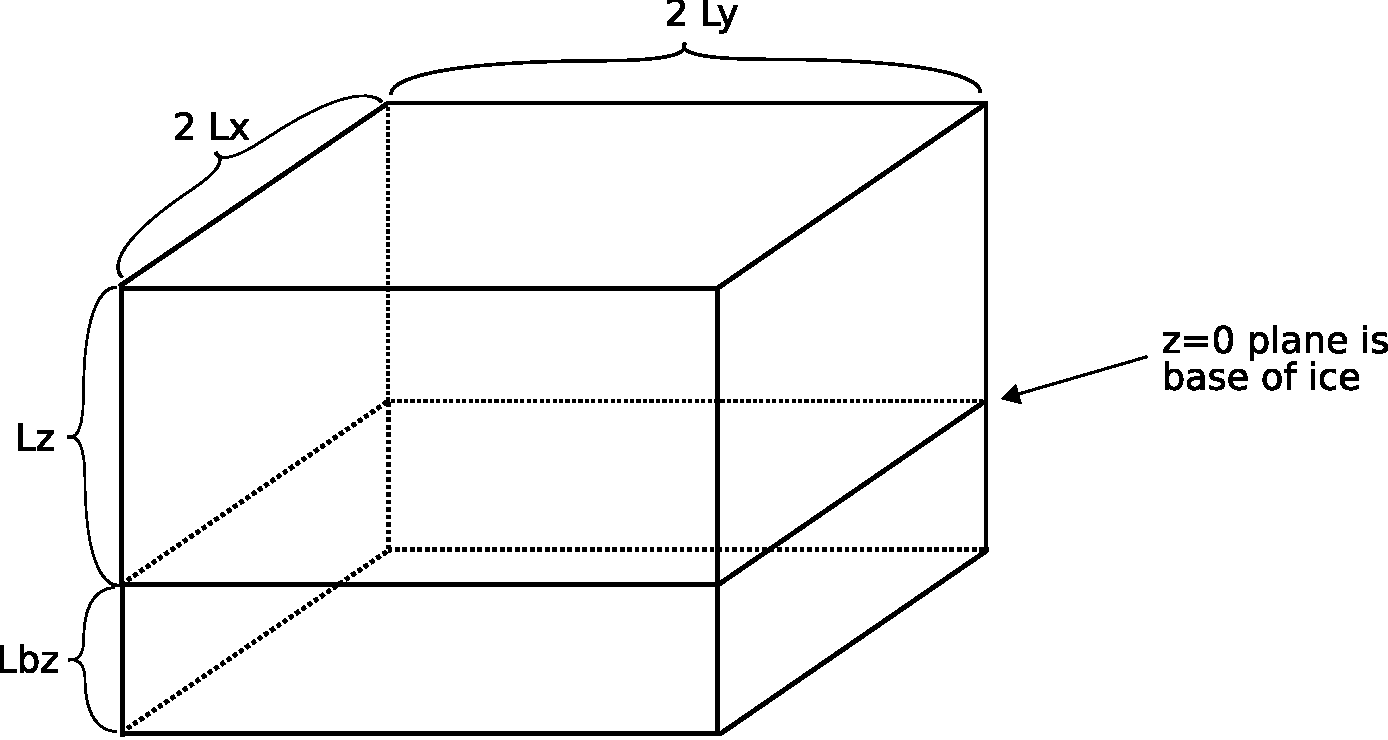
\includegraphics[width=4.0in,keepaspectratio=true]{figs/rectilinearbox}
\caption{PISM's computational box.}
\label{fig:rectilinearbox}
\end{figure}

The extent of the computational box for the ice is directly controlled by the options \intextoption{Lx}, \intextoption{Ly}, and \intextoption{Lz} as described in Appendix 1.  As noted \t{-Lx} and \t{-Ly} options should include values in kilometers while \t{-Lz} should be in meters.

\subsection{Grid} \label{subsect:grid} The PISM grid\index{PISM!grid} covering the computational box is equally spaced in each of the three dimensions.  FIXME: non-equal spacing in vertical allowed with \verb|-quadZ|

Because of the bedrock extension, the grid of points is described by four numbers, namely the number of grid points in the $x$ direction, the number in the $y$ direction, the number in the $z$ direction within the ice, and the number in the $z$ direction within the bedrock.  These are specified by options \intextoption{Mx}, \intextoption{My}, \intextoption{Mz}, and \intextoption{Mbz}, respectively, as described in the Runtime options section.  The defaults for these four values are 61, 61, 31, and 1, respectively.  Note that \verb|Mx|, \verb|My|, \verb|Mz|, and \verb|Mbz| all indicate the number of grid \emph{points}.  Therefore the number of grid \emph{spaces} are, respectively, 60, 60, 30, and 0 (zero) in the default case.  Note that the lowest grid point in a column of ice, that is the one at $z=0$, coincides with the highest grid point in the bedrock.  Also \verb|Mbz| must always be at least one.

The distance \t{Lbz} is controlled by specifying the number \verb|Mbz| of grid points in the bedrock, noting that the vertical spacing \t{dz} is the same within the ice and within the bedrock.  To avoid conflicts, the distance \t{Lbz} cannot be set directly by the user.  In particular, $\text{\t{Lbz}}=\text{\t{dz}}\,(\text{\t{Mbz}}-1)$ while $\text{\t{dz}} = \text{\t{Lz}} / (\text{\t{Mz}}-1)$, and so the distance \t{Lbz} into the bedrock is determined by setting \t{Lz}, \t{Mz}, and \t{Mbz}.

One is allowed to specify the grid when PISM is started \emph{without} a pre-existing model state (i.e.~as stored in a NetCDF input file output by PISM).  For instance, a shortened EISMINT II experiment A \cite{EISMINT00} run, which will produce a convenient NetCDF file for our purposes here, is\index{pisms}

\verb|$  pisms -eisII A -Mx 61 -My 61 -Mz 101 -y 5000 -o foo|

\noindent If one initializes PISM from a saved model state then the input model state controls the parameters \t{Mx}, \t{My}, \t{Mz}, and \t{Mbz}.  For instance, the command

\verb|$  pisms -eisII A -if foo.nc -Mz 201 -y 100|

\noindent will give a warning that ``\verb|user option -Mz ignored; value read from file foo.nc|.''  To change the model grid one must explicitly ``regrid'', as described next.


\subsection{Regridding}  It is common to want to interpolate a coarse grid model state onto a finer grid or vice versa.  For example, one might want to do the EISMINT II experiment as above, producing \verb|foo.nc|, but then interpolate both the ice thickness and the temperature onto a finer grid.  Speaking conceptually, the idea in PISM is that one starts over from the beginning of EISMINT II experiment A on the finer grid, but one extracts the thickness and ice temperature stored in the coarse grid file and interpolates onto the finer grid before proceeding with the actual computation.  The transfer from grid to grid is reasonably general---one can go from coarse to fine or vice versa in each dimension $x,y,z$---but the transfer must always be done by \emph{interpolation} and never \emph{extrapolation}.  (An attempt to do the latter will always produce a PISM error.)

Such ``regridding'' is done using the \intextoption{regrid} and \intextoption{regrid\und vars} commands as in this example:\index{pisms}

\verb|$  pisms -eisII A -Mx 101 -My 101 -Mz 201 -y 1000 \|

\verb|     -regrid foo.nc -regrid_vars HT -o bar|

\noindent By specifying regridded variables ``\verb|HT|'', the ice thickness and temperature values from the old grid are interpolated onto the new grid.  Note that one doesn't need to regrid the bed elevation, which is set identically zero as part of the EISMINT II experiment A description, nor the ice surface elevation, which is computed as the bed elevation plus the ice thickness at each time step anyway.

A slightly different use of regridding occurs when ``bootstrapping'' as described in section \ref{sect:boot} and illustrated by example in section \ref{sect:green}.

See table \ref{tab:regridvar} for the regriddable variables.  Only modeled variables are regriddable, while climate and boundary data is not.

\begin{table}[ht]
\caption{Regriddable variables.\index{regrid}\index{regrid\und vars}  Use \texttt{-regrid$\underline{\phantom{b}}$var} with given flag.}\label{tab:regridvar}
\begin{tabular}{@{}llll}\hline
\textbf{Flag} & \textbf{Name in NetCDF file} & \textbf{Description}\\ \hline
\verb|b| & \texttt{topg}       & bed elevation \\
\verb|B| & \texttt{litho\und temp} & temperature in bedrock \\
\verb|e| & \texttt{age}        & age of the ice \\
\verb|h| & \texttt{usurf}      & surface elevation \\
\verb|H| & \texttt{thk}        & thickness \\
\verb|L| & \texttt{bwat}       & thickness of basal melt water \\
\verb|T| & \texttt{temp}       & ice temperature \\
\hline
\normalsize
\end{tabular}
\end{table}


\subsection{Adaptive time-stepping} \label{subsect:adapt}\index{PISM!adaptive time stepping scheme} Recall that at each time step the PISM standard output includes flags and a summary of the model state using a few numbers.:
\begin{verbatim}
%ybp SIA SSA  # vgatdh Nr  +STEP
P         YEAR:     ivol   iarea    meltf     thick0     temp0
\end{verbatim}
Here we explain what `\verb|Nr|' and `\verb|STEP|' in the flag line mean.

\verb|STEP| is the time step just taken by PISM, in model years.  This time step is determined by a somewhat complicated adaptive mechanism.  Note that PISM does each step explicitly when numerically approximating mass conservation in the map-plane.  This, and the modeling of advection \cite{BBL}, requires and adaptive time-stepping scheme.

Note that most of the time `\verb|N|' in the flag line will be zero.  The exception is when the option \verb|-skip| is used.  If \verb|-skip| $M$ is used, then \verb|N| will be at most $M$, and will countdown the mass conservation steps when the adaptive scheme determines that a long temperature/age evolution time step, relative to the diffusity controlled time step for mass conservation, would be allowed.  To see an example, do:\index{pismv}

\verb|$  pismv -test G -Mx 141 -My 141 -Mz 51 -skip 4|

Table \ref{tab:adaptiveflag} explains the meaning of the one character adaptive-timestepping flag `\verb|r|'.

\begin{table}[ht]
\caption{Meaning of the adaptive time-stepping flag `\texttt{r}' in standard output flag line.}\label{tab:adaptiveflag}
\begin{tabular}{@{}llll}\hline
\textbf{Flag} & \textbf{Active adaptive constraint} \\ \hline
\verb|c| & 3D CFL for temperature/age advection \cite{BBL} \\
\verb|d| & diffusivity for SIA mass conservation \cite{BBL} \\
\verb|e| & end of prescribed run time \\
\verb|f| & \verb|-dt_force| set; generally option \verb|-dt_force|, which overrides the adaptive scheme, \\
 & should not be used  \\
\verb|m| & maximum allowed $\Delta t$ applies; set with \verb|-max_dt| \\
\verb|t| & maximum $\Delta t$ was \emph{t}emporarily set by a derived class; e.g.~see effect of deliverables \\
 & \verb|-time|$n$ in \verb|pisms -ismip H \time|$n$ \\
\verb|u| & 2D CFL for mass conservation in SSA regions (where mass conservation is \emph{u}pwinded)\\
\hline
\normalsize
\end{tabular}
\end{table}


\subsection{Signals, to control a running PISM model} \label{subsect:signal} \index{signals} \index{PISM!catches signals -TERM and -USR1}  Ice sheet model runs sometimes take a long time and the state of the run needs checking.  Sometimes they need to be stopped, but with the possibility of restarting.  PISM implements these behaviors using ``signals'' from the POSIX standard.  Such signals are included in Linux and most flavors of Unix.  Table \ref{tab:signals} below summarizes how PISM responds to signals.

Here is an example.  Suppose we start a long verification run in the background, with standard out redirected into a file:\index{pismv}

\verb|pismv -test G -Mz 101 -y 1e6 -o testGmillion >> log.txt &|

\noindent This run gets a Unix process id (``\verb|pid|''); we will need that number.  (One can get the \verb|pid| by using the \verb|ps| or \verb|pgrep| utilities.)

If we want to observe the run without stopping it we send the \verb|USR1| signal:\index{kill}

\verb|kill -USR1 8920|

\noindent where ``\verb|8920|'' happened to be the \verb|pid| of the running PISM process.  It happens that we caught the run at year 31871.5 or so because a NetCDF file \verb|pism-31871.495239.nc| is produced.  This intermediate state file can be viewed by \verb|ncview pism-31871.495239.nc|.  Note also that in the standard out log file \verb|log.txt| the line

\verb|...|

\verb|Caught signal SIGUSR1: Writing intermediate file `pism-31871.495239.nc'.|

\verb|...|

\noindent appears around time step (i.e.~\verb|YEAR|) 31900.

Suppose, on the other hand, that the run needs to be stopped.  One may use the interrupt ``\verb|kill -KILL 8920|'' for this process, which is running in the background.  (Foreground processes can be interrupted by Ctrl-C.)  This brutal method, which a process cannot catch or block, stops the process but does not allow it  time to save the model state.  Therefore one will not be able to restart at the same place, nor inspect the model state more thoroughly.  If one wants the possibility of restarting then one should used the \verb|TERM| signal,

\verb|kill -TERM 8920|

\noindent Then the PISM run is stopped and the lines

\verb|Caught signal SIGTERM: exiting early.|

\verb|...|

\verb|Writing model state to file `testGmillion.nc' ... done|

\noindent appear in the log file \verb|log.txt|.  In this case the NetCDF model state file \verb|testGmillion.nc| appears; note this file has the original output name specified by the option \verb|-o|.  One can restart and finish the run by the command (for example)

\verb|pismv -test G -if testGmillion.nc -ye 1e6 -o testGmillion_finish >> log_cont.txt &|
\smallskip

Finally we consider a multiple process (MPI) run of PISM.  Here each of the processes must be sent the same signal at the same time.  For example, consider the dialog
\begin{quote}
\begin{verbatim}
	~/pism$ mpiexec -n 4 pismv -test C -y 100000 >> log.txt &
	~/pism$ ps
	PID TTY          TIME CMD
	6761 pts/0    00:00:00 mpiexec
	6762 pts/0    00:00:00 pismv
	6763 pts/0    00:00:00 pismv
	6764 pts/0    00:00:00 pismv
	6765 pts/0    00:00:00 pismv
	6770 pts/2    00:00:00 ps
	~/pism$ kill -USR1 6762 6763 6764 6765
	~/pism$ kill -TERM 6762 6763 6764 6765
\end{verbatim}
\end{quote}
Here the \verb|kill| command sent the signal to all four of the running PISM processes simultaneously.  The \verb|kill -USR1| command caused the NetCDF file \verb|pism-10852.037393.nc| to be written, while \verb|kill -TERM| caused all four processes to end after (collectively, of course) writing \verb|verify.nc|.

If, as in the above situation, one wants to send all \verb|pismv| processes the \verb|-TERM| signal then\index{pkill} 

  \verb|pkill -TERM pismv|

\noindent will have the same effect as \verb|kill -TERM| followed by a list of all the \verb|pid|s of \verb|pismv| processes.

\newcommand\pid{\textsl{pid}}
\newcommand\same{(\textsl{same})}
\begin{table}[ht]
\caption{Signalling PISM.  \pid~stands for list of all identifiers of the running PISM processes.}\label{tab:signals}
\begin{tabular}{@{}llll}\hline
\textbf{Command}\phantom{bobbob} & \textbf{Signal}\phantom{bobbob} & \textbf{PISM behavior} \\ \hline
\texttt{kill -KILL} \pid & \texttt{SIGKILL} & terminate with extreme prejudice; PISM cannot catch it \\
 & & and no state is saved \\
\texttt{kill} -9 \pid & \same & \same \\
Ctrl-C & \same & same, but only for foreground process(es)  \\ \hline
\texttt{kill -TERM} \pid & \texttt{SIGTERM} & end process(es) but save the last model state \\
 &  & using the user-given \verb|-o| name or the default name \\
\texttt{kill} -15 \pid & \same & \same \\
\texttt{kill} \pid & \same & \same \\
\texttt{pkill -TERM pismv} & \same & \same; most convenient for MPI runs \\ 
 &  & to terminate and save) \\ \hline
\texttt{kill -USR1} \pid & \texttt{SIGUSR1} & allow process(es) to continue but save model state \\
 &  & at current time using name \texttt{pism-}\textsl{year}\texttt{.nc} \\
\texttt{pkill -USR1 pismv} & \same & \same; most convenient for MPI runs \\
\hline\normalsize
\end{tabular}
\end{table}


\subsection{Positive degree-day model}  \label{subsect:pdd} \index{positive degree day model} \index{PDD (positive degree day model)} \index{PISM!default positive degree day model}  By default the accumulation/ablation map in PISM is treated as net surface mass balance.  (We are referring to the variable \verb|acab| in saved model states, and to the view \verb|-d a|.)  The mass conservation equation for the ice sheet requires this surface balance, which is in units of meters ice-equivalent per time.

Also, the surface temperature variable in PISM is assumed to be the mean annual surface temperature, and without an additional model or input there is no yearly temperature cycle.

If the input data actually includes the annual snow-fall accumulation then one must \emph{compute} the surface mass balance according to some model of how much of the snow is melted in each model year and according to a yearly temperature cycle.  We call such a model a \emph{positive degree day} model \cite{CalovGreve05}.

The model used by PISM in computing the amount of melting first assumes a sinusoidal temperature cycle over the course of the year, where the difference between the peak of this temperature cycle and its mean (average) is called the ``summer warming.''  The default temperature cycle has a constant amount of summer warming.  This constant is specified by \intextoption{pdd\und summer\und warming}.  Note that the mean temperature is grid-point dependent, as specified by the input surface temperature map (data), so the cycle is different at each map-plane grid location, though the amplitude is the same at each grid point (in this default case).  The peak of the cycle occurs on August 1, which is Julian day 243, but the option \intextoption{pdd\und summer\und peak\und day} can override this.

It is common to add ``white noise'' to the temperature cycle to simulate both the daily temperature cycle and additional variability associated to the vagaries of weather.  More precisely, a normally-distributed, mean zero random temperature increment is added (or subtracted) from the temperature for each day.  These increments are independent over the days of the year, though of course we only have pseudo-randomness \dots, but they are the same over the whole sheet.  Their standard deviation is controlled by \intextoption{pdd\und std\und dev}.

The number of positive degree days, denoted PDD, is computed as the sum of the product of the amount by which this temperature cycle, including the white noise variability, exceeds $0\!\phantom{|}^\circ \text{C}$ times the time (in days) during which it is above zero.  In PISM there are two methods for computing PDD.  The first is the expected value computed by the method described in \cite{CalovGreve05}; this option is chosen by \intextoption{pdd}.  The second is a monte carlo simulation of the white noise itself, chosen by \intextoption{pdd\und rand}.  (If one wants runs with repeatable randomness, use \intextoption{pdd\und repeatable} instead of \verb|-pdd_rand|.)

The PDD is multiplied by a coefficient (set by \intextoption{pdd\und factor\und snow}) to compute the amount of snow melted.  Of this melted snow, a fraction (\intextoption{pdd\und refreeze}) is kept as ice.  This ice, plus all unmelted snow (measured as ice-equivalent) is added to the mass balance unless the PDD exceeds that required to melt all of the snow-fall in the year.  In this latter case, in which there are excess PDD available for melting, the excess PDD is multiplied by a coefficient (\intextoption{pdd\und factor\und ice}) to compute how much ice is melted.  In this latter case, ablation occurs at that location.

The PDD model is applied in section \ref{sect:green} to modeling the Greenland ice sheet.

To directly compare the two methods, try\index{pgrn}

\verb|$ pgrn -bif eis_green_smoothed.nc -Mx 83 -My 141 -Mz 201 \|

\verb|    -ocean_kill -y 50 -o green_50yr_pdd -d Aa|

\noindent versus

\verb|$ pgrn -bif eis_green_smoothed.nc -Mx 83 -My 141 -Mz 201 \|

\verb|    -ocean_kill -y 50 -o green_50yr_pdd_rand -pdd_rand -d Aa|

\noindent (See section \ref{sect:green} on how to create the file \verb|eis_green_smoothed.nc| from publically available data.  See the same section for the meaning of ``\verb|-bif|''.)


\subsection{Floatation criterion and mask} \label{subsect:float} FIXME: add this section to explain semantics of mask, \verb|MASK_FLOATING_OCEAN0|, and \intextoption{ocean\und kill}; add and document option \intextoption{dry}


\subsection{Earth deformation models} \label{subsect:beddef} \index{earth deformation} \index{PISM!earth deformation models, using}   FIXME: add this section, which explains use of options
\intextoption{bed\und def\und iso} and \intextoption{bed\und def\und lc}  Based on papers by Lingle and Clark \cite{LingleClark}\index{Lingle, Craig} \index{Clark, J.} and \cite{BLKfastearth}.  Example runs to compare are is

\verb|$ pisms -eisII A -quadZ -y 6000 -o eisIIA_nobd|

\verb|$ pisms -eisII A -quadZ -bed_def_iso -y 6000 -o eisIIA_bdiso|

\verb|$ pisms -eisII A -quadZ -bed_def_lc -y 6000 -o eisIIA_bdlc|

Also refer to test H.



\clearpage\newpage
\section{Verification}\label{sect:verif}

\bigskip
\begin{quote}  Two types of errors may be distinguished: modeling errors and numerical errors.  modeling errors arise from not solving the right equations.  Numerical errors result from not solving the equations right.  The assessment of modeling errors is \emph{validation}, whereas the assessment of numerical errors is called \emph{verification} \dots  Validation makes sense only after verification, otherwise agreement between measured and computed results may well be fortuitous.
\end{quote}\index{validation versus verification}
\hfill P.~Wesseling, (2001)  \emph{Principles of Computational Fluid Dynamics}, pp.~560--561 \cite{Wesseling}
\bigskip

\subsubsection*{Ideas} ``Verification'' is a crucial task for a code as complicated as PISM.\index{PISM!verification of}  It is the exclusively mathematical and numerical task of checking that the predictions of the numerical code are close to the predictions of the continuum model (the one which the numerical code claims to approximate).  One is not comparing model output to nature.  Instead, one compares exact solutions of the continuum model, in circumstance in which they are available, to the numerical approximations of those solutions.

See \cite{BLKCB} and \cite{BBL} for discussion of verification issues for the isothermal and thermomechanically coupled shallow ice approximation (SIA), respectively, and for exact solutions to these models.  See \cite{SchoofStream} for an exact solution to the SSA equations for ice streams using a plastic till assumption.  Reference \cite{Roache} gives a broad discussion of verification and validation in computational fluid dynamics.

In PISM there is a separate executable \verb|pismv| which is used for verification.  The numerical codes which are verified by \verb|pismv| are, however, exactly the same lines of source code in exactly the same source files as is run by the non-verification executables \verb|pismr|, \verb|pisms|, \verb|pgrn|, etc.  In technical terms, \verb|pismv| runs a derived class of the base class \verb|IceModel|\index{IceModel C++ class and its derived classes}, and \emph{all} PISM executables run \verb|IceModel|.

\begin{table}[ht]
\caption{Exact solutions for verification.}\label{tab:tests}
\small
\begin{tabular}{@{}llll}\hline
\textbf{Test} & \textbf{Continuum model tested} & \textbf{Comments} & \textbf{Reference} \\ \hline
A & isothermal SIA, steady, &  & \cite{BLKCB} \\
 & flat bed, constant accumulation &  &  \\
B & isothermal SIA, flat bed, zero accum & similarity soln & \cite{BLKCB,Halfar83} \\
C & isothermal SIA, flat bed, growing accum & similarity soln & \cite{BLKCB} \\
D & isothermal SIA, flat bed, oscillating accum & compensatory accum & \cite{BLKCB} \\
E & isothermal SIA; as A &  compensatory accum & \cite{BLKCB} \\
 & but with sliding in a sector &  &  \\
F & thermomechanically coupled SIA (mass &  compensatory accum & \cite{BB,BBL} \\
 & and energy cons.), steady, flat bed & and comp~heating &  \\
G & thermomechanically coupled SIA; as F  & ditto & \cite{BB,BBL} \\
 & but with oscillating accumulation &  &  \\
H & bed deformation coupled with isothermal SIA & joined similarity & \cite{BLKfastearth} \\
I & stream velocity computation using SSA (plastic till) &  & \cite{SchoofStream} \\
J & shelf velocity computation using SSA  &  & [IN PREPARATION] \\
K & pure conduction in ice and bedrock & & \cite{BuelerTestK} \\
L & isothermal SIA, steady, non-flat bed & numerical ODE soln & [IN PREPARATION] \\
\hline
\normalsize
\end{tabular}
\end{table}

\begin{table}[ht]
\caption{Running PISM\index{pismv!options to run verification tests}\index{verification tests}  to verify using the exact solutions listed in table \ref{tab:tests}.}\label{tab:tests_exec}
\small
\begin{tabular}{@{}llll}\hline
\textbf{Test} & \textbf{Example invocation}  \\ \hline
A & \verb|pismv -test A -Mx 61 -My 61 -Mz 11 -y 25000| \\
B & \verb|pismv -test B -Mx 61 -My 61 -Mz 11 -ys 422.45 -y 25000|  \\
C & \verb|pismv -test C -Mx 61 -My 61 -Mz 11 -y 15208.0|  \\
D & \verb|pismv -test D -Mx 61 -My 61 -Mz 11 -y 25000|  \\
E & \verb|pismv -test E -Mx 61 -My 61 -Mz 11 -y 25000|  \\
F & \verb|pismv -test F -Mx 61 -My 61 -Mz 61 -y 25000|  \\
G & \verb|pismv -test G -Mx 61 -My 61 -Mz 61 -y 25000|  \\
H & \verb|pismv -test H -Mx 61 -My 61 -Mz 11 -y 40034 -bed_def_iso| \\
I & \verb|pismv -test I -Mx 5 -My 500 -ssa_rtol 1e-6 -ksp_rtol 1e-11| \\
J & \verb|pismv -test J -Mx 60 -My 60 -Mz 11 -ksp_rtol 1e-12| \\
K & \verb|pismv -test K -Mx 6 -My 6 -Mz 401 -Mbz 101 -y 130000| \\
L & \verb|pismv -test L -Mx 61 -My 61 -Mz 31 -y 25000| \\
\hline
\normalsize
\end{tabular}
\end{table}

Table \ref{tab:tests} summarizes the many exact solutions currently available in PISM.  Note that most of these exact solutions are solutions of \emph{free boundary problems} for partial differential equations.  (Tests A, E, J, and K are fixed boundary value problems.)  Table \ref{tab:tests_exec} shows how to run each of them on modestly-refined grids (for relatively quick execution time).

\subsubsection*{Refinement}  To meaningfully verify a numerical code one must go down a grid refinement path and measure numerical error for each grid \cite{Roache}.  By ``a refinement path''\index{refinement path!definition} we mean the specification of a sequence of grid cell sizes which decrease toward the refinement limit.  For example, in the the two spatial and one time dimension case this means a sequence of triples $(\Delta x,\Delta y,\Delta t)$ which decrease toward the (unreachable) refinement limit $(\Delta x,\Delta y,\Delta t) = (0,0,0)$.  By ``measuring the error for each grid'' we will mean computing a norm (or several norms) of the difference between the numerical solution and the exact solution.   Concretely, we will typically compute both the \emph{maximum} numerical error anywhere on the grid and the \emph{average} numerical error on the grid.

The goal is not to see that the error is zero at any stage on the refinement path, or even that the error is small in a predetermined absolute sense, generally.  Rather the goal is to see that the error is trending toward zero, and to measure the rate at which it decays.  Knowing the error decay rate allows the modeler to have a sense of how fine a grid is necessary to achieve a small enough numerical error so that the numerical solution can be regarded as a (near) solution to the continuum model.  See \cite{BLKCB,BBL,Roache,Wesseling}.

For an example of a refinement path, consider the runs\index{refinement path!example}\index{pismv}
\begin{quote}\small\begin{verbatim}
pismv -test B -ys 422.45 -y 25000 -Mx 31 -My 31 -Mz 11
pismv -test B -ys 422.45 -y 25000 -Mx 61 -My 61 -Mz 11
pismv -test B -ys 422.45 -y 25000 -Mx 121 -My 121 -Mz 11
pismv -test B -ys 422.45 -y 25000 -Mx 241 -My 241 -Mz 11
\end{verbatim}
\normalsize\end{quote}
These verify the basic function of the isothermal shallow ice approximation components of PISM in the case of no accumulation.  The exact solution used here is the Halfar similarity solution \cite{Halfar83}.  Note that one specifies the number of grid points when running PISM, but this is equivalent to specifying the grid cell sizes if the overall dimensions of the computational box is fixed; see subsection \ref{subsect:coords}.  The refinement path is the sequence of triples $(\Delta x,\Delta y,\Delta t)$ with $\Delta x = \Delta y = 80,40,20,10$ and where $\Delta t$ is determined adaptively by a stability criterion (see subsection \ref{subsect:adapt}).  Note that the vertical grid spacing $\Delta z$ is fixed because this test is isothermal and no dependence of the error is expected from changing $\Delta z$.

The data produced by the above four runs appears in figures 7, 8, 9, and 10 of \cite{BLKCB}.  We see there that the isothermal mass conservation scheme does a reasonable job of approximating the evolving surface.  Future improvements in the numerical scheme may make the error decrease faster or be smaller.

For thermocoupled tests one refines in three dimensions.  For example, the runs\index{refinement path!example}
\begin{quote}\small\begin{verbatim}
pismv -test G -max_dt 10.0 -y 25000 -Mx 61 -My 61 -Mz 61
pismv -test G -max_dt 10.0 -y 25000 -Mx 91 -My 91 -Mz 91
pismv -test G -max_dt 10.0 -y 25000 -Mx 121 -My 121 -Mz 121
pismv -test G -max_dt 10.0 -y 25000 -Mx 181 -My 181 -Mz 181
pismv -test G -max_dt 10.0 -y 25000 -Mx 241 -My 241 -Mz 241
pismv -test G -max_dt 10.0 -y 25000 -Mx 361 -My 361 -Mz 361
\end{verbatim}
\normalsize\end{quote}
produced figures 13, 14, and 15 of \cite{BBL}.  (The last couple of these runs required a supercomputer!  The $361\times 361\times 361$ run involves more than $100$ million unknowns, updated at each of millions of time steps.)

\subsubsection*{Results}  Figures \ref{fig:thickerrsB} through \ref{fig:temperrsK} show a sampling of the results of verifying PISM using the tests described above.\index{PISM!verification results and reporting}  These figures were produced more-or-less automatically using Python scripts \verb|test/verifynow.py|\index{verifynow.py} and \verb|test/vnreport.py|\index{vnreport.py}.  See appendix \ref{sect:scripts}.

\begin{figure}[ht]
\includegraphics[width=4.8in,keepaspectratio=true]{figs/thickerrs_B}
\caption{Numerical thickness errors in test B.  Vertical axis is in meters. ``maxH error'' is the maximum thickness error anywhere on the grid, ``avH error'' is the average thickness error anywhere on the grid, and ``centerH error'' is the error at the center of the ice sheet.  See \cite{BLKCB} for discussion.}
\label{fig:thickerrsB}
\end{figure}

\begin{figure}[ht]
\includegraphics[width=4.8in,keepaspectratio=true]{figs/thickerrs_G}
\caption{Numerical thickness errors in test G.  Meaning exactly as in test C.  See \cite{BBL} and \cite{BLKCB} for discussion.}
\label{fig:thickerrsG}
\end{figure}

\begin{figure}[ht]
\includegraphics[width=4.8in,keepaspectratio=true]{figs/temperrs_G}
\caption{Numerical temperature errors in test G.  Vertical axis is in Kelvin.  ``maxT'' and ``basemaxT'' errors are maximum over all points within the ice and over all the basal points, respectively.  Similarly for ``avT'' and ``baseavT''; these are average errors.  See \cite{BBL} for discussion.}
\label{fig:temperrsG}
\end{figure}

\begin{figure}[ht]
\includegraphics[width=4.8in,keepaspectratio=true]{figs/surfvelerrs_G}
\caption{Numerical errors in computed surface velocities in test G.  Vertical axis is in meters per year.}
\label{fig:surfvelerrsG}
\end{figure}

\begin{figure}[ht]
\includegraphics[width=4.8in,keepaspectratio=true]{figs/velerrs_I}
\caption{Numerical errors in horizontal velocities in test I, an ice stream.  Vertical axis is in meters per year.  See \cite{SchoofStream} for a description of the exact solution.}
\label{fig:velerrsI}
\end{figure}

\begin{figure}[ht]
\includegraphics[width=4.8in,keepaspectratio=true]{figs/temperrs_K}
\caption{Numerical temperature errors in test K, which tests the thermal bedrock model.  Vertical axis is in Kelvin.  ``maxT'' and ``avT'' are errors computed over all points within the ice while ``maxTb'' and ``avTb'' are computed over all grid points within the bedrock.  See \cite{BuelerTestK} for a discussion.}
\label{fig:temperrsK}
\end{figure}


\clearpage\newpage
\section{Simplified geometry experiments}\label{sect:simp}

\subsection{Historical note}  There have been three stages of ice sheet model intercomparisons based on simplified geometry experiments since the early 1990s \cite{BuelerSpray}.\index{EISMINT!defined}

EISMINT\footnote{``EISMINT'' stands for European Ice Sheet Modeling INiTiative.  

See \texttt{http://homepages.vub.ac.be/\%7Ephuybrec/eismint.html}.} I \cite{EISMINT96} was the first of these and involved only the isothermal shallow ice approximation (SIA).  Both fixed margin and moving margin experiments were performed in EISMINT I, and various conclusions were drawn about the several numerical schemes used in the intercomparison.  EISMINT I is superceded, however, by \emph{verification} using the full variety of known exact solutions to the isothermal SIA, as shown in \cite{BLKCB}.  The ``rediscovery'', since EISMINT I, of the Halfar similarity solution with zero accumulation \cite{Halfar83} is a particular reason why good performance on the ``moving margin'' experiment in EISMINT I is, roughly speaking, irrelevant.  For this reason there has been no attempt to support the EISMINT I experiments in PISM, although it would be easy code to write.

EISMINT II \cite{EISMINT00} was both a more significant and more controversial intercomparison.  It pointed out interesting and surprising properties of the thermocoupled SIA.  References \cite{BBL,Hindmarsh04,Hindmarsh06,PayneBaldwin,SaitoEISMINT} each interpret the EISMINT II experiments and/or describe attempts to add more complete physical models to ``fix'' the (perceived and real) shortfalls of ice sheet models as evidenced by their behavior on EISMINT II experiments.  PISM has built-in support for all of the published and unpublished EISMINT II experiments; these are described in the next subsection.

The ISMIP\footnote{``ISMIP'' stands for Ice Sheet Model Intercomparison Project.  \index{ISMIP!defined}

See \texttt{http://homepages.vub.ac.be/\%7Ephuybrec/ismip.html}.} round of intercomparisons are ongoing at this time.  There are two components of ISMIP substantially completed, namely HOM = Higher Order Models \cite{HOMtcd,HOMelmer} and HEINO = Heinrich Event INtercOmparison \cite{GreveTakahamaCalov}.

Of these ISMIP experiments, PISM participated in HEINO, but this ability is unmaintained.  The results from PISM for HEINO are not regarded by the PISM authors as any more or less meaningful than those from other participating models.\index{ISMIP!interpretation of HEINO results}   We believe the continuum problem described by HEINO is not easily approximate-able because of a (large) discontinuous jump in the basal velocity field.  The continuum problem predicts infinite vertical velocity \cite[][Appendix B]{BBssasliding}, and the same phenomenon occurs in the EISMINT II experiment H continuum problem.  Details of the numerical schemes and their results are irrelevant if the continuum model makes such a prediction.  In essence, PISM offers the results in \cite{BBssasliding} as an alternative to HEINO results.

There is no current plan to support ISMIP-HOM.

A third ISMIP part is the Marine Ice Sheet Model Intercomparison Project (MISMIP)\index{ISMIP!MISMIP}.  It is supported in PISM, as described in subsection \ref{subsect:MISMIP}.


\subsection{EISMINT II in PISM}\label{subsect:EISMINTII}  There are seven experiments described in the published EISMINT II writeup \cite{EISMINT00}.\index{EISMINT}  They are labeled A, B, C, D, F, G, and H.  As specified in the writeup, the common features of all of these experiments are:\begin{itemize}
\item runs are of 200,000 years, with no prescribed time step;
\item runs are on a prescribed $61\times 61$ horizontal grid;
\item the boundary conditions always have angular symmetry around the center of the grid;
\item the bed is flat and does not move (there are no isostasy effects);
\item the temperature in the bedrock is not modeled;
\item only shallow ice approximation physics is included;
\item the change in the temperature of ice is described by the shallow approximation of the conservation of energy \cite{Fowler};
\item thermomechanical coupling is included, both because of the temperature dependence of the softness of the ice, \emph{and} through the strain-heating (dissipation-heating) term in the conservation of energy equation;
\item the ice is \emph{cold} and not \emph{polythermal} \cite{Greve}; and finally
\item though basal melt rates may be computed diagnostically, they do not contribute to the dynamics of the ice sheet.
\end{itemize}
The experiments differ from each other in their various combinations of surface temperature and accumulation parameterizations.  Also, experiments H and G involve basal sliding, while the others don't.  Four experiments start with zero ice (A,F,G,H), while the other experiments (B,C,D) start from the final state of experiment A.

In addition to the seven experiments published in \cite{EISMINT00}, there were an additional five experiments described in the EISMINT II intercomparison description 
\cite{EISIIdescribe}, labeled E, I, J, K, and L.\index{EISMINT!unpublished additional EISMINT II experiments}  These experiments share most features, itemized above, but with the following differences.  Experiment E is the same as experiment A except that the peak of the accumulation, and also the low point of the surface temperature, are shifted by 100 km in both $x$ and $y$ directions; also experiment E starts with the final state of experiment A.  Experiments I and J are similar to experiment A but with non-flat topography.  Experiments K and L are similar to experiment C but with non-flat topography.  See table \ref{tab:eisII} for how to run these experiments.

The vertical grid is not specified in the EISMINT II writeup.  It seems that good simulation of the complex thermomechanically coupled conditions near the base of the ice requires relatively fine resolution there.  Because PISM (currently) has an equally-spaced grid, we recommend the use of about 200 vertical levels.  Thus a reasonable experiment A run on one processor is

\verb|pisms -eisII A -Mx 61 -My 61 -Mz 201 -y 200000 -o eisIIA|

\noindent The SIA-only simulations parallelize well, and we see speedups up to 30 or more processors (for the standard $61\times 61$ horizontal grid).

Table \ref{tab:eisII} shows how each of the EISMINT II experiments can be done in PISM.

\begin{table}[ht]
\caption{Running the EISMINT II experiments in PISM;\index{PISM!running the EISMINT II experiments in} the command is ``\t{pisms}'' plus the given options.  Experiments below the horizontal line are only documented in \cite{EISIIdescribe}.}\label{tab:eisII}
\small
\begin{tabular}{@{}llll}\hline
\textbf{Command: ``\t{pisms}'' $+$} & \textbf{Relation to experiment A} \\ \hline
\verb|-eisII A -Mx 61 -My 61 -Mz 201 -y 2e5 -o eisIIA| & \\
\verb|-eisII B -if eisIIA.nc -y 2e5 -o eisIIB| & warmer \\
\verb|-eisII C -if eisIIA.nc -y 2e5 -o eisIIC| & less snow (lower accumulation)\\
\verb|-eisII D -if eisIIA.nc -y 2e5 -o eisIID| & only smaller area of accumulation \\
\verb|-eisII F -Mx 61 -My 61 -Mz 201 -y 200000 -o eisIIF| & colder; famous spokes \cite{BBL} \\
\verb|-eisII G -Mx 61 -My 61 -Mz 201 -y 200000 -o eisIIG| & sliding (regardless of temperature) \\
\verb|-eisII H -Mx 61 -My 61 -Mz 201 -y 200000 -o eisIIH| & melt-temperature activated sliding \\ \hline
\verb|-eisII E -if eisIIA.nc -y 2e5 -o eisIIE| & shifted accumulation/temperature maps \\
\verb|-eisII I -Mx 61 -My 61 -Mz 201 -y 2e5 -o eisIII| & trough topography \\
\verb|-eisII J -if eisIII -y 2e5 -o eisIIJ| & trough topography and less snow \\
\verb|-eisII K -Mx 61 -My 61 -Mz 201 -y 2e5 -o eisIIK| & mound topography \\
\verb|-eisII L -if eisIIK -y 2e5 -o eisIIL| & mound topography and less snow \\
\hline\normalsize
\end{tabular}\end{table}

The EISMINT II experiments can be run with various modifications of the default settings.  Of course the grid can be refined.  For instance, a twice as fine grid in the horizontal is ``\t{-Mx 121 -My 121}''.  Table \ref{tab:eisIIoptions} lists some optional settings which are particular to the EISMINT II experiments.  With the exception of ``\verb|-Lz|'', these options will only work if option ``\t{-eisII ?}'' is also set.

\begin{table}[ht]
\caption{Changing the default settings for the EISMINT II experiments in PISM.\index{PISM!special options for EISMINT II experiments}}\label{tab:eisIIoptions}
\small
\begin{tabular}{@{}llll}\hline
\textbf{Option} & \textbf{Default values [expers]} & \textbf{Units} & \textbf{Meaning} \\ \hline
\verb|-Mmax| & 0.5 [ABDEFGHIK], 0.25 [CJL] & m$/$a & max value of accumulation rate \\
\verb|-Rel| & 450 [ABEFGHIK], 425 [CDJL] & km & radial distance to equilibrium line \\
\verb|-Sb| & $10^{-2}$ [\emph{all}] & (m/a)/km & radial gradient of accumulation rate \\
\verb|-ST| & $1.67 \times 10^{-2}$ [\emph{all}] & K/km & radial gradient of surface temperature\\
\verb|-Tmin| & 238.15 [ACDEGHIJKL], & K & max of surface temperature \\
 & 243.15[B], 223.15[F] & & \\
\verb|-track_Hmelt| &  &  & compute effective thickness of basal melt \\
 &  &  & water (override default for EISMINT II) \\
\verb|-Lz| & 4500 [AE], 4000 [BCD], & m & height of the computational box \\
 & 5000 [F], 3000 [G] &  &  \\
\hline\normalsize
\end{tabular}\end{table}

Note that in PISM the height \verb|Lz| of the computational box is fixed at the beginning of the run.  On the other hand, changing the boundary conditions of the flow, as for instance by setting option \verb|-Mmax| to a larger than default value (see table \ref{tab:eisIIoptions}), may cause the ice sheet to thicken above the \verb|Lz| height.  If the ice grows above the height of the computational box then a ``\verb|Vertical grid exceeded!|'' or ``\verb|thickness overflow in SIA velocity: ks>Mz!|'' error occurs.  This can be fixed by restarting with a larger value for option \verb|-Lz|.\footnote{Automatic rescaling of, or expansion of, the vertical grid is appropriate, but not yet implemented.}


\begin{comment}
\subsection{ISMIP-HEINO in PISM}  The goal of the ISMIP-HEINO intercomparison is to evaluate the degree to which the thermomechanically coupled shallow ice approximation with basal sliding is a model for the surge behavior of the Laurentide ice sheet which is believed to have caused the ``Heinrich events'' described in [CITE HEINRICH].  Further information about HEINO, including the intercomparison description [URL FOR HEINO PDF] can be found at \url{http://www.pik-potsdam.de/~calov/heino.html}.

HEINO involves eight different runs of 200,000 years on a prescribed $81\times 81$ grid in the horizontal.  As in EISMINT II there is no prescription of vertical grid.  During the entirety of each run certain integrated quantities (area, melted base area, etc.) and other quantities measured at prescribed basal points must be reported at each year into ASCII files with \verb|.dat| extensions.  During the last 50,000 years of each of the eight runs, a map-plane (``planform'') dump of other quantities must be made to additional \verb|.dat| ASCII files.  These latter dumps must be made at the time of maximum and minimum extents of various quantities and the only way to determine the time of maximum/minimum extents is to complete the 200,000 year runs, determine the times of maximum and minimums, and then rerun the last 50,000 years from the saved state at 150,000 years.  See the intercomparison description [CITE URL for PDF].

PISM handles all the difficult details of the procedures described in the previous paragraph, but it is important for the user to have a sense for what is supposed to be reported.

HEINO is a relatively expensive intercomparison in terms of computer time.  For this reason use of a multiprocessor machine is recommended though not essential.  If the intercomparison participant's initials were X.~Y.~Z.~then a HEINO run ST is the recipe

\verb|mpiexec -n 8 pisms -ismip H -run ST -Mx 81 -My 81 -Mz 281 \|

\verb|    -y 150000 -dat_prefix XYZ_START -o XYZ_ST_150k|

\verb|mpiexec -n 8 pisms -ismip H -run ST -if XYZ_ST_150k.nc \|

\verb|    -y 50000 -dat_prefix XYZ_END -o XYZ_ST_200k|

[use Matlab to determine max/min]

\verb|mpiexec -n 8 pisms -ismip H -run ST -if XYZ_ST_150k.nc \|

\verb|    -y 50000 -time1 -time2 -time3 -time4 -dat_prefix XYZ_RERUN|

\verb|~/pism/test/heinocatdat.sh XYZ_ST_??? ...|

\verb|~/pism/test/renames.sh | [rename planform files?]

\noindent At the end of the above recipe the files [list] should appear.

\begin{table}[ht]
\caption{Options used in running ISMIP-HEINO in PISM.}\label{tab:heinooptions}
\small
\begin{tabular}{@{}llll}\hline
\textbf{Option} & \textbf{Default value(s)} & \textbf{Comments} \\ \hline
\verb|-| & & \\
\verb|-| & & \\
\verb|-dat_prefix| & \verb|PISM| & put initials here \\
\verb|-| & & \\
\verb|-ismip| & \verb|H| & only HEINO implemented for now \\
\verb|-| & & \\
\verb|-| & & \\
\verb|-| & & \\
\hline\normalsize
\end{tabular}\end{table}
\end{comment}


\subsection{MISMIP in PISM}\label{subsect:MISMIP}  This intercomparison is described at the webpage

\centerline{\url{http://homepages.ulb.ac.be/~fpattyn/mismip/}}

\noindent The full text description, available at the above site as PDF, is essential reading to understand MISMIP results.


\begin{table}[ht]
\caption{MISMIP run options in PISM.\index{PISM!special options for MISMIP experiments}}\label{tab:MISMIPoptions}
\small
\begin{tabular}{@{}lll}\hline
\textbf{Option} & \textbf{Default value} & \textbf{Meaning} \\ \hline
\verb|-extras| &  & if this flag is set then, once steady state is reached,  \\
               &  & surface elevation and bed elevation are written to \\
               &  & an extra file with name ending \verb|_extras|\\
\verb|-initials| & \verb|ABC| & initials to prepend to ASCII output file names \\
\verb|-mismip| & \verb|1a| & experiment number followed by sliding flag; \\
               &  & allowed values are \verb|1a,1b,2a,2b,3a,3b| \\
\verb|-model| & 1 & model 1 is SSA only an is ``category 1'' in the \\
              &   & MISMIP classification; model 2 combines SIA and SSA \\
              &   & velocities as described in \cite{BBssasliding} \\
\verb|-steady_atol| & \verb|1.0e-4| & m/a; tolerance for steady state;  \\
                    & & criterion is $\|dH/dt\|_\infty <$(\verb|steady_atol| value) \\
\verb|-step| & 1 & allowed values are $\{1,\dots,9\}$ for experiment 1,  \\
             &  & $\{1,\dots,13\}$ for exper.~2, and $\{1,\dots,15\}$ for exper.~3;  \\
             &  & note typo in table 6 in PDF: ``step 16'' is mentioned \\
             &  & but only 15 values are given \\
\hline\normalsize
\end{tabular}\end{table}


FIXME: MORE




\clearpage\newpage
\section{Example: Modeling the Greenland ice sheet}\label{sect:green} \index{PISM!running the EISMINT Greenland intercomparison}\index{Greenland ice sheet}\index{EISMINT!intercomparison of Greenland models} In this section we give an extended example of how to use PISM to model the Greenland ice sheet.  We use somewhat stale data from the 1990s ice sheet modelling intercomparison known as EISMINT-Greenland \cite{HuybrechtsEISMINT,RitzEISMINT}.  Though based on old data, EISMINT-Greenland serves as an excellent tutorial example.

The data for performing this experiment are freely available at
\medskip

\centerline{\protect{\textbf{\url{http://homepages.vub.ac.be/~phuybrec/eismint/greenland.html}}}}
\medskip

\noindent The snow-fall accumulation map, ablation parameterization, surface temperature formula, surface elevation, and bedrock elevation maps are essentially as in the 1991 papers \cite{Letreguillyetal1991,OhmuraReeh}.  Note that in the ice and sea floor-core driven ``forced climate'' run \verb|-ccl3| described below, the ice sheet is forced by changes in temperature from the GRIP core \cite{Dansgaardetal1993} and by changes in sea level from SPECMAP \cite{Imbrieetal1984}.  A parameter-sensitivity study of a EISMINT-Greenland type ice sheet model is described in \cite{RitzFabreLetreguilly}.

Substantial developments have occurred in modeling the Greenland ice sheet since the EISMINT-Greenland intercomparison.  For example, the relation between a Greenland ice sheet flow model, Earth deformation under ice sheet loads, and the reconstruction of global ice loading is analyzed in \cite{TarasovPeltier}.  The response of Greenland ice sheet models to climate warming is addressed in \cite{HuybrechtsdeWolde,Huybrechts02, Greve00}, among other references.


\subsubsection*{Obtaining and converting EISMINT-Greenland data}  We use two Python scripts to convert the EISMINT-Greenland data, which is in the form of several ASCII text files, into NetCDF files usable by PISM.  The Python libraries \href{http://numpy.scipy.org/}{\texttt{numpy}} and \href{http://code.google.com/p/netcdf4-python/}{\texttt{netcdf4-python}} must be present for the scripts to work.

First, \verb|cd examples/eisgreen/| from the PISM directory, and download these text (ASCII) files from the EISMINT-Greenland web site above: 

\verb|grid20-EISMINT,  suaq20-EISMINT,  specmap.017,  sum89-92-ss09-50yr.stp|

\noindent One method for the download is: \small

\verb|$  for name in "grid20-EISMINT" "suaq20-EISMINT" "specmap.017" "sum89-92-ss09-50yr.stp"|

\verb|>   do  wget http://homepages.vub.ac.be/~phuybrec/eismint/$name;  done|

\normalsize\noindent Once all four files have been downloaded, run

\verb|$ ./eis_green.py|

\noindent The NetCDF file \verb|eis_green20.nc| will be created from the data in \verb|grid20-EISMINT| and \verb|suaq20-EISMINT|.  It contains variables for the gridded latitude (\verb|lat|), longitude (\verb|lon|), surface altitude (``\verb|usurf|'' for \emph{u}pper \emph{surf}ace elevation), bedrock altitude (\verb|topg|), ice thickness (\verb|thk|), and snow accumulation rate (\verb|acab|).  These values can be viewed graphically with \verb|ncview|.  The header (metadata) can be viewed by \verb|ncdump -h eis_green20.nc|.

\begin{comment}
If needed, the script \verb|eis_green.py| accepts option \verb|--prefix=foo/| if the downloaded data is in directory \verb|foo/|; \verb|eis_core.py| below also takes this option.  Option \verb|-g| specifies grid spacing; use \verb|-g 40| if you downloaded \verb|grid40-EISMINT| and \verb|suaq40-EISMINT| 40 km data; ``\verb|-g 20|'' or no option specifies 20 km grid.

As an exercise, the \href{http://nco.sourceforge.net/}{\texttt{NCO}} can be used on \verb|eis_green20.nc| to compare the putative ice surface elevation to the sum of the ice thickness and the bed elevation:

\verb|$ ncap -O -vs "check=usurf-(thk+topg)" eis_green20.nc eis_green_check.nc|

\noindent The variable \verb|check| in the output file holds the difference of \verb|usurf| and the sum $\verb|topg|+\verb|thk|$.  Viewing \verb|check| in \verb|ncview| will show that \verb|usurf| is within 1 meter of $\verb|topg|+\verb|thk|$.  Thus the surface elevation \verb|usurf| is consistent.  It is also redundant because at bootstrapping, described below, PISM reads ice thickness and bed elevation and computes ice surface elevation as the sum of these two.
\end{comment}

The bed elevation in the original data (\verb|suaq20-EISMINT|) effectively contains a missing value attribute of $0.0$, because in several places---deep fjords, mostly---the observed bed elevation was not measured or the measured value was not trusted.  When viewing \verb|eis_green20.nc| with \verb|ncview|, these values show as white spots.  If these missing values are left in then the bed elevation map is extraordinarily rough and this makes reasonable ice flow predictions more difficult.  We therefore smoothly fill the holes in the bed elevations.  This is done with another script named \verb|fill_missing.py|,\footnote{Requires \href{http://code.google.com/p/netcdf4-python/}{\texttt{netcdf4-python}}.  It is a general tool for smoothly filling patches of missing values in variables in NetCDF files.  It looks for attributes defining missing values and then fills in specified variables essentially by averaging the neighboring non-missing values.  See Appendix D.} found in directory \verb|pism/util/|:

\verb|$ fill_missing.py -f eis_green20.nc -v topg -o eis_green_smoothed.nc|

\begin{figure}[ht]
\includegraphics[width=2.6in,keepaspectratio=true]{figs/EISgreen_thick}\qquad\includegraphics[width=2.8in,keepaspectratio=true]{figs/EISgreen_bed}
\caption{Views of the thickness (left) and smoothed bed elevation (right) for EISMINT-Greenland.  The coastal topography around several fjords has been smoothed..}
\label{fig:greendata}
\end{figure}

In addition to getting the EISMINT gridded data into NetCDF format and filling missing values, there is an issue with Ellesmere Island.  Ellesmere Island is very close to Greenland, and so it would be possible for the modeled ice sheet to flow onto it.  (Indeed this presumably occurred at the last glacial maximum.)  Since we don't, however, have correct topography or accumulation rates for Ellesmere Island among the downloaded data \cite{RitzEISMINT}, we want to prevent this from happening.  Therefore special code is executed by the PISM executable \verb|pgrn| which we use below.  It says that all points northwest of the line connecting the points $(68.18^\circ E, 80.1^\circ N)$ and $(62^\circ E, 82.24^\circ N)$ are removed from the flow simulation.  The same applies to anything east of $30^\circ E$ and south of $67^\circ N$ so that the flow could not spread to the tip of Iceland (not likely anyway \dots).  The phrase ``removed from the flow simulation'' actually means that the points are marked as ice-free ocean; the use of option \verb|-ocean_kill| below means that ice-free ocean remains that way.

Next we use the script which converts the data files \verb|specmap.017| and \verb|sum89-92-ss09-50yr.stp| to  PISM readable NetCDF form:

\verb|$ ./eis_core.py|

\noindent Two NetCDF files with one-dimensional (time series) data will be created, namely \verb|grip_dT.nc| and \verb|specmap_dSL.nc|.  The executable \verb|pgrn| will be called with options \verb|-dTforcing| and \verb|-dSLforcing| for these two \verb|.nc| files in the ``CCL3'' run below.  Thus PISM reads the GRIP data \cite{Dansgaardetal1993} for the surface temperature forcing and the SPECMAP data \cite{Imbrieetal1984} form sea level forcing.  Figure \ref{fig:gripDeltaT} shows the GRIP temperature offsets.

\begin{figure}[ht]
\includegraphics[width=5.6in,keepaspectratio=true]{figs/gripDeltaT}
\caption{Change in temperature from present, from the GRIP core.  A famous graph reproduced by applying \texttt{ncview} to \texttt{grip\und dT.nc}}
\label{fig:gripDeltaT}
\end{figure}


\subsubsection*{Bootstrapping from EISMINT-Greenland data}  Once the EISMINT Greenland data is obtained and converted to NetCDF, as above, ``bootstrapping'' can begin.  By ``bootstrapping'' we mean the creation, by heuristics and simplified models, of the kind of full initial conditions needed for the continuum model (differential equations) inside PISM.\footnote{Section \ref{sect:boot} will explain, once written, that ``bootstrapping'' is a form of inverse modeling, and that we must inevitably do inverse modeling to do prognostic ice sheet modeling.}

Table \ref{bootstrapEISgreen} shows the entire PISM output for a one model year run using option \verb|-bif| to ``bootstrap'' from file \verb|eis_green_smoothed.nc|\index{pgrn}

\verb|$ pgrn -bif eis_green_smoothed.nc -Mx 141 -My 83 -Lz 4000 -Mz 51 -quadZ \|

\verb|  -ocean_kill -skip 0 -y 1 -o green20km_y1|

\noindent The run takes a few seconds of real time.

\begin{table}\label{bootstrapEISgreen}
\scriptsize
\begin{quote}
\begin{verbatim}
$  pgrn -bif eis_green_smoothed.nc -Mx 141 -My 83 -Lz 4000 -Mz 51 -quadZ \
   -ocean_kill -skip 0 -y 1 -o green20km_y1
PGRN (EISMINT Greenland mode)
bootstrapping by PISM default method from file eis_green_smoothed.nc
  all dimensions t,x,y,z,zb found in file
  time t = 0.0000 years found; setting current year
  rescaling computational box *for ice* from defaults, -bif file, and
    user options to dimensions:
    [-1400.00 km, 1400.00 km] x [-820.00 km, 820.00 km] x [0 m, 4000.00 m]
  polar stereographic var found; attributes present: svlfp=1, lopo=1, sp=1
     values: svlfp = -41.14, lopo =  71.65, sp =  71.00
  variable lon found and regridded; min,max =  -94.194,  12.889 (degrees_east)
  variable lat found and regridded; min,max =   58.275,  84.458 (degrees_north)
  variable acab found and regridded; min,max =    0.030,   2.820 (m a-1)
  variable thk found and regridded; min,max =    0.000,3200.000 (m)
  variable topg found and regridded; min,max = -3859.000,2151.000 (m)
  WARNING: ignoring values found for surface elevation 'usurf';
    using usurf = topg + thk
  WARNING: effective thickness of basal melt water 'bwat' not found;
    using default constant  0.000 m
  WARNING: surface temperature 'artm' not found; using default constant 263.15 K
  WARNING: till friction angle 'tillphi' not found; using default constant 15.000 degrees
  WARNING: geothermal flux 'bheatflx' not found; using default constant  0.042 W/m^2
  WARNING: uplift rate 'dbdt' not found; using default constant  0.000 m/s
  determining mask by floatation criterion:  grounded ice and ice-free
    land marked as 1, floating ice as 3, ice free ocean as 7
  filling in temperatures at depth using quartic guess
done reading eis_green_smoothed.nc; bootstrapping done
resetting vertical levels base on options and user option -Lz ...
using PDD based on standard yearly surface temp cycle
geothermal flux set to EISMINT-Greenland value 0.050000 W/m^2
computing surface temps by EISMINT-Greenland elevation-latitude rule
filling in temperatures at depth using quartic guess
removing extra land (Ellesmere and Iceland) using EISMINT-Greenland rule
  [computational box for ice: ( 2800.00 km) x ( 1640.00 km) x ( 4000.00 m)]
  [hor. grid cell dimensions: (   20.00 km) x (   20.00 km)]
  [vertical grid spacing in ice not equal: 21.200 m < dz < 138.800 m]
  [fine equal spacing used in temperatureStep(): Mz = 190, dzEQ = 21.164 m]
P         YEAR:     ivol   iarea    meltf     thick0     temp0
U        years 10^6_km^3 10^6_km^2 (none)          m         K
S      0.00000:  2.82500  1.6708   0.2071   3042.000  270.5156
 $$ SIA        v [BPsacr=2.6660%] atdh 0d  +0.18299
S      0.18299:  2.82515  2.2300   0.1683   3041.886  270.5156
 $$ SIA        v [BPsacr=2.4695%] atdh 0d  +0.23532
S      0.41832:  2.82534  2.2296   0.1681   3041.699  270.5157
 $$ SIA        v [BPsacr=2.1875%] atdh 0d  +0.26959
S      0.68791:  2.82521  1.6832   0.2058   3041.450  270.5159
 $$ SIA        v [BPsacr=1.9653%] atdh 0d  +0.29938
S      0.98729:  2.82525  1.6840   0.2055   3041.163  270.5161
 $$ SIA        v [BPsacr=1.7090%] atdh 0e  +0.01271
S      1.00000:  2.82526  2.2288   0.1680   3041.151  270.5164
done with run ... 
Writing model state to file `green20km_y1.nc'
\end{verbatim}
\end{quote}
\normalsize
\bigskip

\caption{Bootstrapping from the EISMINT-Greenland data and running for one model year.}
\end{table}

Let's explain what has happened.  The EISMINT-Greenland data, as with \emph{all} real ice sheet data, does not contain certain variables necessary to initialize PISM in the sense of complete initial values for time-dependent partial differential equations.  For instance, the data do not include the temperature of the ice anywhere but at the surface (and only there by a elevation and latitude dependent formula).  The data also do not include the amount of water stored in the till, for instance.  These are not omissions from the data sets but rather inevitable facts; one cannot observe ice sheets as fluids very well.  Therefore PISM fills in the unknown initial conditions based on some default guesses, as indicated by the messages in Table \ref{bootstrapEISgreen}.

Note that EISMINT-Greenland specifies an 83 by 141 point grid, but you may use other numbers for \verb|-Mx| and \verb|-My| if desired.  In such cases the data will be linearly interpolated onto your grid.  Larger values will produce slower runs.

\begin{comment}
But there is a transpose: In order to make the diagnostic viewers described in Appendix \ref{sect:viewers} have the correct orientation, the x and y axes are switched internally in PISM.  Of course the physics approximated by PISM does not care about orientation.  The consequence of using ``\verb|-Mx 83 -My 141|'', instead of the correct pair shown, would be to have grid cells which are far from square, and to have squashed viewers.
\end{comment}

The option \verb|-bif| stands for ``bootstrapping input file''.  This option is an alternative to \verb|-if| (stands for ``input file'') which is used for a file which has full initial conditions.  In practice, \verb|-if| is only used with a NetCDF file which was previously saved by PISM; that is, \verb|-if| is used to continue a run from a saved state.

Note the choice of the height of the computational box (``\verb|-Lz 4000|''), of the number of vertical levels (``\verb|-Mz 51|''), and of a not-equally-spaced grid (``\verb|-quadZ|'').  The messages to standard out show that the vertical spacing is less than 30 m near the base and more than 130 m at the top of the computational box (where it matters less).

Regarding the temperature within the ice, bootstrapping applies an interpolation scheme to the surface temperatures and geothermal fluxes.  It is based on a heuristic for the amount of downward flow in a column.  Bootstrapping creates a temperature field at depth.\footnote{See the PISM \emph{Reference Manual} for a formula.}

This bootstrapping mode also fills in several default values.  For instance, the variables \verb|bheatflx| (geothermal flux), \verb|dbdt| (bed uplift rate), and \verb|bwat| (effective thickness of basal water) were not found in the input file, whereas they would be in a saved PISM model state.  Also, note that the EISMINT Greenland data had redundant surface elevation values; PISM bootstrapping includes the computation ``\verb|usurf = topg + thk|'' of the surface elevation from the ice thickness and the bed elevation.

Continuing with the above output, after default bootstrapping there are additional settings special to EISMINT-Greenland.  For instance, because there is no EISMINT-Greenland gridded data set for surface temperature \cite{RitzEISMINT}, at the surface there is a formula which determines the temperature as a function of latitude and surface elevation.  The code behind \verb|pgrn| knows this formula and uses it.  The constant value for geothermal flux is reset, and the above-mentioned Ellesmere Island issue is resolved.

\subsubsection*{Relaxing the temperature field}  Before seeking a good steady state for the entire thermo-mechanically-coupled ice sheet, it is helpful to do a better job of filling in the temperatures within the ice.  One way to do this is to have the temperature field and velocity field co-evolve according to the thermomechanical flow model, but while holding the upper ice surface stationary.  This is a continuation of ``bootstrapping''.  The effect is to replace the heuristic temperature field applied above by one which is approximately stationary with respect to advection and conduction.  The resulting temperature field is still not the fully physical temperature field, however, because it comes from a steadiness assumption about position of the surface of the ice.

We create this temperature field by running for 10000 years\footnote{In fact a much longer run should be done for serious modeling because the exponential time constant for decay of the thermomechanically-coupled system toward equilibrium is on the order of 100k years.} with non-evolving surface, using the option \verb|-no_mass| to turn off the map-plane mass continuity scheme:

\verb|$ mpiexec -n 2 pgrn -if green20km_y1.nc -no_mass -y 10000 -o green20km_Tsteady|

\noindent This last run takes on the order of one processor hour.  Many more processors are effective, up to perhaps peak real time speed with 40 to 80 processors for this 83 by 141 grid.  Note finer grid computations are easier to parallelize in the sense that greater maximum speedup over one processor, in wall clock time, is attainable.

The EISMINT-Greenland experiments \cite{RitzEISMINT} specify a positive degree day (PDD) model which is automatically turned on when using the \verb|pgrn| executable.  (Other executables may require option \verb|-pdd| or \verb|-pdd_rand| to turn on the PDD model.)  The PDD model is, by default, implemented by the deterministic scheme described in \cite{CalovGreve05}, but the user can add option \verb|-pdd_rand| to use a stochastic PDD model.

\subsubsection*{Running the EISMINT-Greenland steady state experiments}  Now that we have initial conditions including a vaguely-credible temperature field, our first experiment is the steady state run ``SSL2''.  This experiment uses the parameters specified in the EISMINT-Greenland description \cite{RitzEISMINT}.  If 8 processors are used, a ten thousand model year run might look like this:

\verb|mpiexec -n 8 pgrn -ssl2 -if green20km_Tsteady.nc -y 10000 -ys 0 -ocean_kill \|

\verb|     -o green_SSL2_10k >> ssl2.txt|

\noindent We can continue for another ten thousand years by

\verb|mpiexec -n 8 pgrn -ssl2 -if green_SSL2_10k.nc -y 10000 -ocean_kill \|

\verb|     -o green_SSL2_20k >> ssl2.txt|

Note the option ``\verb|-ocean_kill|''.  This forces all floating ice to immediately calve off (i.e.~to have thickness zero).  (Compare the Ross ice shelf model in the next section.)

These runs took about 15 minutes each on an 2 quad core Xeon server (2008 technology).  This simulation is, however, intended to go until the model reaches a ``steady state'', a phrase which \cite{RitzEISMINT} defines as a small volume change rate, namely less than a .01\% change in volume in 10,000 years.

One can look at the standard output text file by a minimal method like ``\verb|less ssl2.txt|''.  But, to more clearly see the behavior over time of the volume, area, basal melt fraction, and so on, one can generate a time series file in NetCDF form and then use various tools to view and manipulate that file.  Use the Python script \verb|util/series.py|, documented in Appendix D, like this:

\verb|$  series.py -f ssl2.txt -o ssl2_series.nc|

\noindent View using \verb|ncview|, for instance.  One sees that the volume shows a consistent growing-but-leveling-out trend, with a final volume expected to be a bit more than $4 \times 10^{6}\,\text{km}^3$.

In fact that is what happens with a long run.  If we run the SSL2 experiment with the specified ``0.01\% change in 10k years'' criterion, then the run ends at 110k years with a volume change of about 0.001\% between the 100k and 110k model states.  This steady state criteria can be most easily determined by examining the time series NetCDF file produced by \verb|series.py| (from a completed partial run or even during an ongoing run).  The final volume was $4.087 \times 10^{6}\,\text{km}^3$.  The time series for volume and melt fraction (the fraction of the base where the temperature is at pressure-melting) are shown in Figures \ref{fig:eisgrnvolseries} and \ref{fig:eisgrnmeltfseries}.  The volume time series is boring, but the melt fraction indicates something interesting: measured by basal melt fraction, the temperature field resulting from bootstrapping and relaxing the temperature field (above) gave a pretty good estimate of the basal melt fraction for the fully coupled steady state.

\begin{figure}[ht]
\includegraphics[width=6.0in,keepaspectratio=true]{figs/eisgrn_volseries}
\caption{Volume time series for a 110k model year EISMINT-Greenland run; units of $10^{6}\,\text{km}^3$.}
\label{fig:eisgrnvolseries}
\end{figure}

\begin{figure}[ht]
\includegraphics[width=6.0in,keepaspectratio=true]{figs/eisgrn_meltfseries}
\caption{Time series for the fraction of the base which is at the pressure-melting temperature from a 110k model year EISMINT-Greenland run.  See the right hand part of Figure \ref{fig:ssl2thickThomol} for a map of the basal temperature.}
\label{fig:eisgrnmeltfseries}
\end{figure}

The command that completed the full 110k model year run is 

\verb|mpiexec -n 8 pgrn -ssl2 -if green_SSL2_20k.nc -y 90000 -ocean_kill \|

\verb|     -o green_SSL2_110k >> ssl2.txt|

We will use the final NetCDF file \verb|green_SSL2_110k.nc| to continue the EISMINT-Greenland experiments below.  The saved ice thickness and homologous basal temperature maps are shown in Figure \ref{fig:ssl2thickThomol}.  The vertically-averaged horizontal velocity is shown in Figure \ref{fig:ssl2cbar}.

\begin{figure}[ht]
\includegraphics[height=3.5in]{figs/greenH_SSL2}\qquad\includegraphics[height=3.5in,width=2.6in]{figs/greenThomol_SSL2}%\includegraphics[height=3.7in,width=2.9in]{figs/greenThomol_SSL2}
\caption{Ice thickness (meters; left) and homologous basal temperature (degrees C below 0; right) at the end (110k model years) of a EISMINT-Greenland SSL2 run.  Note that in the temperature graph the pressure-melting temperature areas are white.}
\label{fig:ssl2thickThomol}
\end{figure}

\begin{figure}[ht]
\includegraphics[height=3.5in,keepaspectratio=true]{figs/greencbar_SSL2}
\caption{Vertically-averaged horizontal velocity in meters per year at the end (110k model years) of a EISMINT-Greenland SSL2 run.}
\label{fig:ssl2cbar}
\end{figure}

In addition to the more standardized EISMINT-Greenland intercomparison called ``SSL2'', a ``SSL3'' was proposed to allow each participant to choose additional parameters and adjust other aspects of the model.  (Sliding, for instance, is an outstanding omission here.)  We omit this run for tutorial purposes, however, and proceed to use climate forcing in runs ``CCL3'' and ``GWL3''.


\subsubsection*{Climate forcing from GRIP and SPECMAP}  The next experiment starts from the end of the steady state run above.  Recall that the NetCDF files \verb|grip_dT.nc| and \verb|specmap_dSL.nc| contain time series data for change in surface temperature and sea level.  The options \verb|-dTforcing| and \verb|-dSLforcing| include these data for a ``CCL3'' climate forced run \cite{RitzEISMINT,HuybrechtsEISMINT}.  Before every time step, \verb|pgrn| reads the change to the surface temperature and sea level for that time.  The data in \verb|grip_dT.nc| extends 250,000 years into the past, while the data in \verb|specmap_dSL.nc| goes back about 780,000 years, so EISMINT-Greenland specifies that the run will start at the beginning of the GRIP data.  Thus we manually set the starting year using the option \verb|-ys|:

\verb|$  pgrn -ccl3 -if green_SSL2_110k.nc -dTforcing grip_dT.nc \|

\verb|      -dSLforcing specmap_dSL.nc -ys -249900 -ye 0 -o green_CCL3_y0|

\noindent Note option \verb|-ccl3| also turns on the Lingle and Clark \cite{BLKfastearth,LingleClark} two layer, flat earth bed deformation model with an assumption of zero uplift rate at the start of the run.

The resulting thickness difference, relative to the end of the SSL2 run, and the homologous basal temperature, are shown in Figure \ref{fig:cclthickThomol}.

\begin{figure}[ht]
\includegraphics[width=3.3in]{figs/Hdiff_CCLSSL}\,\includegraphics[width=3.3in]{figs/Thomol_CCL}
\caption{Left:  Ice thickness difference between end (year zero) of a CCL3 run and the end of an SSL2 run (meters).  Right:  Ice homologous basal temperature (degrees C below 0; right) at the end of a EISMINT-Greenland CCL3 run.  Compare Figure \ref{fig:ssl2thickThomol}.}
\label{fig:cclthickThomol}
\end{figure}

EISMINT-Greenland also calls for a baseline run for another 500 years which starts from the end of the CCL3 run and has steady current climate forcing (noting no GRIP or SPECMAP data are known from the future!):

\verb|$  pgrn -ccl3 -if green_CCL3_y0.nc -y 500 -o green_CCL3_y500|


\subsubsection*{A greenhouse warming scenario}  A final ``greenhouse warming'' experiment ``GWL3'' is described in the EISMINT-Greenland \cite{RitzEISMINT}.  It runs for 500 years with the temperature increasing by $0.035^\circ C/$year for the first 80 years, then at a rate of $0.0017^\circ C/$year for the last 420 years:

\verb|$  pgrn -gwl3 -if green_CCL3_y0.nc -y 500 -o green_GWL3_y500|



\clearpage\newpage
\section{Example: Validating PISM as a flow model for the Ross ice shelf}\label{sect:ross} \index{PISM!running the EISMINT Ross ice shelf intercomparison in}\index{Antarctic ice sheet!Ross ice shelf} \index{EISMINT!intercomparison of Ross ice shelf models} \index{PISM!validation of ice shelf model} \index{Ross ice shelf} The term ``validation'' describes the comparison of model output with physical observations in cases where those physical observations are believed to be sufficiently complete and of sufficient quality so that the performance of the numerical model can be assessed \cite{Roache,Wesseling}.  Roughly speaking, validation can happen when the observations or data are better than the model, so the comparison measures the quality of the numerical model, not merely errors in, incompleteness of, or lack of confidence in the data.

As part of the first EISMINT series of intercomparisons, MacAyeal and others \cite{MacAyealetal} validated several ice shelf numerical models using the Ross ice shelf as an example.  We will refer to this intercomparison and its associate write-up \cite{MacAyealetal} as ``EISMINT-Ross''.  The models were compared to data from the RIGGS (= Ross Ice shelf Geophysical and Glaciological Survey) \cite{RIGGS2,RIGGS1}, data acquired in the period 1973--1978.   The RIGGS data include the (horizontal) velocity of the ice shelf measured at a few hundred locations in a reasonably regular grid across the shelf; see figure \ref{fig:rosspython} below for an indication of these positions.

Substantial developments have occurred in the modeling of the Ross ice shelf since the EISMINT-Ross intercomparison.  For example, inverse modeling techniques were used to recover depth-averaged viscosity of the Ross ice shelf from the RIGGS data in \cite{RommelaereMacAyeal}. A parameter-sensitivity study was performed for a particular Ross ice shelf numerical model in \cite{HumbertGreveHutter}.

\subsubsection*{Grabbing the data}  Download data files from the website

\centerline{\url{http://homepages.vub.ac.be/~phuybrec/eismint/iceshelf.html}}

\noindent to do the validation:\small

\verb|$ cd examples/eisross/|

\verb|$ wget http://homepages.vub.ac.be/~phuybrec/eismint/111by147Grid.dat|

\verb|$ wget http://homepages.vub.ac.be/~phuybrec/eismint/kbc.dat|

\verb|$ wget http://homepages.vub.ac.be/~phuybrec/eismint/inlets.dat|

\normalsize\noindent The reader might want to look at these files in a text editor; their idiosyncratic format is handled by the python script \verb|eis_ross.py| (more below).  In fact, a very significant part of setting up EISMINT-Ross in PISM was the step of converting these text files into machine-readable and metadata-containing NetCDF.  Note that these data are for a particular rectangular grid with $6.822$km spacing in both $x$ and $y$ directions, but, as usual, the PISM computational grid can be determined by the user.

The script\footnote{Requires \href{http://numpy.scipy.org/}{\texttt{numpy}} and \href{http://code.google.com/p/netcdf4-python/}{\texttt{netcdf4-python}}.} \verb|eis_ross.py| reads the above three \verb|.dat| files and it creates a NetCDF file:

\verb|$ ./eis_ross.py -o ross.nc|

\noindent Note that the NetCDF file \verb|ross.nc| can be reconverted to text (CDL) using \verb|ncdump| or it can be viewed graphically with \verb|ncview|.  For example,

\verb|$ ncdump -h ross.nc|

\noindent shows the ``header'' (the metadata) for \verb|ross.nc|.  The script \verb|eis_ross.py| has added this metadata, much of which can only be found in \cite{RIGGS2,RIGGS1,MacAyealetal}; attention to such details is unavoidable!

\begin{figure}[ht]
\includegraphics[height=2.3in,keepaspectratio=true]{figs/rossmask} \qquad \includegraphics[height=2.3in,keepaspectratio=true]{figs/rossubar}
\caption{Two views from \protect{\texttt{ncview}} of the EISMINT-Ross data in the NetCDF file \protect{\texttt{ross.nc}}.  The floating-versus-grounded mask (left; red areas are floating ice shelf) and the $x$-component of the non-zero kinematic (Dirichlet) boundary condition for velocity (right).}
\label{fig:rossmaskubar}
\end{figure}

The NetCDF file \verb|ross.nc| contains ice thickness, bed elevations, surface temperature, and accumulation.  Values for latitude and longitude from the RIGGS survey grid \cite{RIGGS1} are given.  All of these are typical of ice sheet modeling data, both in evolution and diagnostic runs.  The file also has variables \verb|ubar| and \verb|vbar|.  These give the boundary values which are needed for the diagnostic computation of velocity, and they are only valid at grounding line locations.  They are the measured velocities of the ice flow inputs to the ice shelf.  Also present are integer variables \verb|mask|, which shows the domain where the ice shelf is modeled, and \verb|bcflag|, which shows the locations where the boundary conditions are to be applied.  Finally, \verb|ross.nc| contains variables which allow us to partly validate our computation.  There is an interger variable \verb|accur| which flags the region where the interpolated measured velocities are believed to be accurate enough for validation.\footnote{\texttt{111by147.dat} has a ``Reliable Velocity Obs'' flag.}  The variables \verb|azi_obs| and \verb|mag_obs| are believed to be accurate in this region \cite{MacAyealetal}.

The original EISMINT-Ross data are on a 111 by 147 grid but \verb|eis_ross.py| extends this grid to a more convenient 147 by 147 grid with the same $6.822$ km spacing in each coordinate direction.  This grid has ice-free ocean beyond the calving front; the calving front is straightened in the EISMINT-Ross intercomparison \cite{MacAyealetal}.

\subsubsection*{Diagnostic computation of ice shelf velocity}  A basic Ross ice shelf velocity computation from these data is:

\verb|$ pismd -ross -bif ross.nc -ssaBC ross.nc -Mx 147 -My 147 -Lz 1000 -Mz 11 \|

\verb|    -ssa -o rossComputed|

\noindent Here we bootstrap (\verb|-bif|; see section \ref{sect:boot}) from \verb|ross.nc|.  We also use a special option \verb|-ssaBC| to specify \verb|ross.nc| as the source of the boundary value data for the ice shelf equations, as mentioned in the last paragraph.  The computational grid specified here is the $6.822$ km data grid in EISMINT-Ross with 147 grid points in each direction.  The maximum thickness of the ice is 874 m so we choose a height for the computational box (\verb|-Lz|) large enough to contain the ice.  Note that using a small number of vertical levels (\verb|-Mz 11|) is reasonable because the EISMINT-Ross intercomparison specifies that the temperature at each depth is just the surface temperature \cite{MacAyealetal}.  In fact there is no thermocoupling issue because the ice hardness used here is constant.

At the end of this run the computed velocity field is compared to the interpolated observed velocities stored in \verb|ross.nc|.  The value called ``average relative error in vector vel'' is most relevant.  A value of 0.07 here means that the averaged absolute difference between the computed and the observed velocity, in the ``accurate'' region, is 7\%.

The output file \verb|rossComputed.nc| contains vertically-averaged horizontal speed in the variable \verb|cbar|.  Viewing that variable will show a picture like the one on the cover page of this \emph{User's Manual}, and like that in figure \ref{fig:rossspeed}.

\begin{figure}[ht]
\includegraphics[height=3.2in,keepaspectratio=true]{figs/rossspeed}
\caption{Computed horizontal ice speed of the Ross ice shelf.  Color gives velocity in m/a; see scale.}
\label{fig:rossspeed}
\end{figure}

There are many variations on this basic ``\verb|pismd -ross|''\pismoptionindex{ross} run above.  First of all one can get more information during the run by adding diagnostic viewers and a more complete (verbose) report to standard out:\index{pismd} \pismoptionindex{ssaBC}\pismoptionindex{pause} \pismoptionindex{ssa}

\verb|$ pismd -ross -bif ross.nc -ssaBC ross.nc -Mx 147 -My 147 -Lz 1000 -Mz 11 \|

\verb|     -ssa -d cnmu -verbose -pause 10|

\noindent Secondly one might want to do the run in parallel and do it on a finer grid.  For example,

\verb|$ mpiexec -n 4 pismd -ross -bif ross.nc -ssaBC ross.nc -Mx 201 -My 201 \|

\verb|     -Lz 1000 -Mz 3 -ssa|

\noindent The result is very similar, as it should be.  On the other hand, since the data is only on a 6.8 km grid we expect no added accuracy on this new 5km grid.

Alternately one might want to experiment with different values of the hardness parameter.  Its default value is $\bar B = 1.9 \times 10^8 \, \text{Pa}\, \text{s}^{1/3}$ as in \cite{MacAyealetal}.   We can also use lower (more severe) tolerances for the nonlinear iteration (\intextoption{ssa\und rtol}) and the linear iteration (\intextoption{ksp\und rtol}) to get more confidence in the numerical scheme:

\verb|$ pismd -ross -bif ross.nc -ssaBC ross.nc -Mx 147 -My 147 -Lz 1000 -Mz 11 -ssa \|

\verb|    -constant_hardness 1.8e8 -ssa_rtol 1e-6 -ksp_rtol 1e-10 -o ross_out_1p8|

\noindent Table \ref{tab:rossoptions} lists some of the options which are useful for this kind of diagnostic velocity computation.

\small
\begin{table}[ht]
\caption{Non-obvious options available and/or recommended with \texttt{pismd -ross}.\index{PISM!options for \texttt{pismd -ross}}}\label{tab:rossoptions}
\begin{tabular}{@{}llll}\hline
\textbf{Option} & \textbf{Explanation/Comments} \\ \hline
  \verb|-d cnmu| &       a good way to see what is going on \\
  \verb|-mato foo -matv cnmuvH|\pismoptionindex{mato}\pismoptionindex{matv} &  writes some model results to \\
    & Matlab-readable file \verb|foo.m| \\
  \verb|-pause N| &      pause for N seconds when refreshing viewers \\
  \verb|-ross| &         only use with executable \verb|pismd| \\
  \verb|-verbose 4| &      shows information on nonlinear iteration and Krylov solve \\
    & and parameters related to solving the ice shelf equations \\
\hline
\end{tabular}
\end{table}
\normalsize


\subsubsection*{Comparison to RIGGS data}  The file \verb|riggs_clean.dat| is a cleaned-up version of the original RIGGS\index{RIGGS} data \cite{RIGGS1, RIGGS2}.  (See \texttt{README} for more explanation on this RIGGS data.)  To convert this data to a NetCDF file, as needed next, do

\verb|$ ./eis_riggs.py -o riggs.nc|

\noindent A file \verb|riggs.nc| will be created.  This data is one-dimensional; it is just a lists of values which have an index dimension \verb|count| in the NetCDF file \verb|riggs.nc|.

Now, \verb|pismd -ross| can read this data and compute a $\chi^2$ statistic comparing computed PISM output to the data:

\small\begin{verbatim}
$ pismd -ross -bif ross.nc -ssaBC ross.nc -Mx 147 -My 147 -Lz 1000 -Mz 3 -ssa -riggs riggs.nc
PISMD (diagnostic velocity computation mode)
initializing EISMINT Ross ice shelf velocity computation ...
. . .
maximum computed speed in ice shelf is   1249.107 (m/a)
. . .
comparing to RIGGS data in riggs.nc ...
Chi^2 statistic for computed results compared to RIGGS is   3625.099
 ... done.
\end{verbatim}
\normalsize

Naturally, the question is ``does this $\chi^2$ value of $3625.099$ represent a good fit of model result to observations''?  Also naturally, there is no objective answer.  For comparison, Table 1 in \cite{MacAyealetal} is reproduced here as Table \ref{tab:chisqr}.  As noted, all these results are with a constant hardness parameter $\bar B = 1.9 \times 10^8 \, \text{Pa}\, \text{s}^{1/3}$ \cite{MacAyealetal}.  The maximum computed horizontal ice speed above of $1249.107$ m/a is lower than the maximum velocities reported by the other models but, on the other hand, the maximum measured speed in the RIGGS data set is $1007$ m/a (near the calving front, of course).  The $\chi^2$ result is essentially as good as the best in the Table, noting smaller $\chi^2$ is better.

\small
\begin{table}[ht]
\caption{Model performance index, $\chi^2$ (non-dimensional).  \protect{\textsl{(Reproduction of Table 1 in \cite{MacAyealetal}.)}}}\label{tab:chisqr}
\begin{tabular}{@{}llll}\hline
\textsl{Model} & $\chi^2$ & \textsl{Maximum velocity} \\
 & & $\text{m}\,\text{a}^{-1}$ \\ \hline
Bremerhaven1 & 3605 & 1379 \\
Bremerhaven2 & 12\,518 & 1663 \\
Chicago1 & 5114 & 1497 \\
Chicago2 & 5125 & 1497 \\
Grenoble & 5237 & 1508 \\
\hline
\end{tabular}
\end{table}
\normalsize

\subsubsection*{Tuning the ice hardness for a better fit to RIGGS}  Because there is a relatively rich data set from RIGGS on ice velocity, it is reasonable to ask whether the PISM computed velocities can fit the data better if the hardness parameter $\bar B$ is adjusted.  There is a Python script \verb|tune.py| which (by default) runs \verb|pismd -ross| with six values of $\bar B$ ranging from $\bar B = 1.5  \times 10^8$ to $\bar B = 2.0 \times 10^8 \, \text{Pa}\, \text{s}^{1/3}$.  It uses smaller values for the convergence tolerances (by default), and it can be run with multiple processors:

\small\begin{verbatim}
$ ./tune.py -n 2
TUNE.PY (for EISMINT Ross; compare to table 1 in MacAyeal et al 1996)
trying "mpiexec -n 2 pismd -ross -bif ross.nc -ssaBC ross.nc -riggs riggs.nc
-ksp_rtol 1e-08 -ssa_rtol 1e-05 -Mx 147 -My 147 -Lz 1000 -Mz 3 -ssa
-constant_hardness 1.5e8"
  finished in 116.7409 seconds; max computed speed and Chi^2 as follows:
  |maximum computed speed in ice shelf is   2355.752 (m/a)
  |Chi^2 statistic for computed results compared to RIGGS is  28157.4
. . .
trying "mpiexec -n 2 pismd -ross -bif ross.nc -ssaBC ross.nc -riggs riggs.nc
-ksp_rtol 1e-08 -ssa_rtol 1e-05 -Mx 147 -My 147 -Lz 1000 -Mz 3 -ssa
-constant_hardness 1.8e8"
  finished in 114.4815 seconds; max computed speed and Chi^2 as follows:
  |maximum computed speed in ice shelf is   1437.704 (m/a)
  |Chi^2 statistic for computed results compared to RIGGS is   3967.9
trying "mpiexec -n 2 pismd -ross -bif ross.nc -ssaBC ross.nc -riggs riggs.nc
-ksp_rtol 1e-08 -ssa_rtol 1e-05 -Mx 147 -My 147 -Lz 1000 -Mz 3 -ssa
-constant_hardness 1.9e8"
  finished in 104.6139 seconds; max computed speed and Chi^2 as follows:
  |maximum computed speed in ice shelf is   1249.716 (m/a)
  |Chi^2 statistic for computed results compared to RIGGS is   3624.1
. . .
\end{verbatim}
\normalsize

We see that hardnesses $\bar B = 1.8,1.9 \times 10^8 \, \text{Pa}\, \text{s}^{1/3}$ give the best fits.  This fitting exercise is a first small step towards inverse modelling of the spatially-distributed effective viscosity.  More steps in such directions are found in \cite{HumbertGreveHutter,RommelaereMacAyeal}


\subsubsection*{Additional visualization}  The visualization abilities of PISM's runtime viewers, and of \verb|ncview| for NetCDF files, are limited.  On the other hand, we can produce pretty pictures using Python with \verb|netcdf4-python| and \verb|matplotlib|; the script \verb|ross_plot.py|\footnote{Requires \t{matplotlib}, \t{scikits.delaunay} and \t{netcdf4-python}.} provides an example.

Assuming that \verb|rossComputed.nc| was produced by the following PISM run

\verb|$ pismd -ross -bif ross.nc -ssaBC ross.nc -Mx 147 -My 147 -Lz 1000 -Mz 11 \|

\verb|    -ssa -o rossComputed|

\noindent and the RIGGS data is in \verb|riggs_clean.dat| described above,

\verb|$ ./ross_plot.py --pism-output=rossComputed.nc --riggs=riggs_clean.dat|

\noindent produces Figure \ref{fig:rosspython}.  We have succeeded in modeling a real ice shelf.

% Alternatively, PISM can save certain variables in a \Matlab-readable form, and this is a situation where it might be useful.\index{PISM!visualizing results}

% \verb|$ pismd -ross -bif ross.nc -ssaBC ross.nc -riggs riggs.nc \|

% \verb|    -ksp_rtol 1e-08 -ssa_rtol 1e-05 -Mx 147 -My 147 -Lz 1000 -Mz 3 -ssa \|

% \verb|    -constant_hardness 1.9e8 -mato ross1p9 -matv cuvHm|

% \noindent When this completes, make sure \Matlab can find \verb|ross1p9.m| and also files \verb|ross_plot.m| and \verb|riggs_clean.dat| (both in directory \verb|pism/test/ross/|).  Execute the \verb|m|-files at the \Matlab command line:

% \verb|>> ross1p9|

% \verb|>> ross_plot|

% \noindent Figure \ref{fig:rosspython} is the result.  We have succeeded in modeling a real ice shelf.

\begin{figure}[ht]
\mbox{\includegraphics[width=3.5in,keepaspectratio=true]{figs/rossquiver}\, \includegraphics[width=3.2in,keepaspectratio=true]{figs/rossscatter}}
\caption{\protect{\emph{Left}}: Color is speed in m/a.  Arrows are observed (black) and computed (red) velocities at RIGGS points.  \protect{\emph{Right}}: Comparison between modeled and observed speeds at RIGGS points; compare figure 2 in \cite{MacAyealetal}.}
\label{fig:rosspython}
\end{figure}


\clearpage\newpage
\section{Inside PISM: overviews of continuum models and numerical schemes}\label{sect:over}

This section is an executive summary.  Technical documentation of the continuum models, numerical methods, and the source code structure is in the PISM \emph{Reference Manual}.\index{PISM!\emph{Reference Manual}}

\subsection{The continuum models in PISM}  Significant features of the continuum model approximated by the PISM include:\index{PISM!continuum models inside}\begin{itemize}
\item The thermocoupled shallow ice approximation equations \cite{Fowler} is verifiably \cite{BLKCB,BBL} solved.
\item Ice shelves and ice streams are modeled by shallow equations which describe flow by longitudinal strain rates and basal sliding.  These equations are different from the shallow ice approximation.  In shelves and streams the velocities are independent of depth within the ice.  The equations were originally established for ice shelves \cite{Morland,MorlandZainuddin,MacAyealetal,WeisGreveHutter}.  They were adapted for ice streams, as ``dragging ice shelves,'' by MacAyeal \cite{MacAyeal}; see also \cite{HulbeMacAyeal,SchoofStream}.  The solution is verifiable using ice stream and ice shelf exact solutions.
\item The regions of grounded ice in which the ice stream model is applied can be determined from a plastic till assumption and the associated free boundary problem \cite{SchoofStream}.
\item A three dimensional age field is computed.
\item A temperature model for the bedrock under an ice sheet is included and geothermal flux which varies in the map-plane can be used.
\item Within the shallow ice sheet regions the model can use the constitutive relation of Goldsby and Kohlstedt \cite{GoldsbyKohlstedt,Peltieretal}.  For inclusion in this flow law, grain size can be computed using a age-grain size relation from the Vostok core data \cite{VostokCore}, for example.
\item The Lingle-Clark \cite{BLKfastearth,LingleClark} bed deformation model can be used.  It generalizes the better known elastic lithosphere, relaxing asthenosphere (``ELRA'') model \cite{Greve2001}.  This model can be initialized by an observed bed uplift map \cite{BLKfastearth}, or even an uplift map computed by an external model like that in \cite{IvinsJames2005}.\end{itemize}

Many of the parts of the model described above are optional.  For instance, options can choose between five different flow laws; see Appendix \ref{sect:options} for options.

The following features are \emph{not} included in the continuum model, and would (or will) require major additions:
\begin{itemize}
\item Inclusion of all components of the stress tensor through either an intermediate order scheme (e.g.~\cite{Blatter,Hindmarsh06,Pattyn03}) or the full Stokes equations \cite{Fowler}.
\item A model for water--content within the ice.  In the current model the ice is \emph{cold} and not \emph{polythermal}; compare \cite{Greve}.  (On the other hand, in the current model the energy used to melt the ice within a given column, if any, is conserved.  In particular, a layer of basal melt water evolves by conservation of energy in the column.  This layer can activate basal sliding and its latent heat energy is available for refreezing.)
\item A model for basal water mass conservation in the map-plane; compare \cite{JohnsonFastook}.
\item A fully spherical Earth deformation model, for example one descended from the Earth model of \cite{Peltier}.
\end{itemize}


\subsection{The numerical schemes in PISM}  Significant features of the numerical methods in PISM include:\index{PISM!numerical methods inside}\begin{itemize}
\item Verification \cite{Roache} is a primary concern and is built into the code.  Nontrivial verifications are available for isothermal ice sheet flow \cite{BLKCB}, thermocoupled sheet flow \cite{BB,BBL}, conservation in ice and bedrock \cite{BuelerTestK}, the earth deformation model \cite{BLKfastearth}, the coupled (ice flow)/(earth deformation) system in an isothermal and pointwise isostasy  case \cite{BLKfastearth}, ice shelf flow (preprint), and ice stream flow based on a plastic bed \cite{SchoofStream}.
\item The code is \emph{structurally} parallel because the PETSc toolkit is used at all levels \cite{petsc-user-ref}.  PETSc manages the MPI-based communication between processors.  It provides an interface to parallel numerical linear algebra.
\item The grid can be chosen at the command line.  Regridding can be done at any time, for example taking the result of a rough grid computation and interpolating it onto a finer grid or vice versa.
\item A moving boundary technique is used for the temperature equation which does not stretch the vertical in a singular manner; the Jenssen \cite{Jenssen} change of variables is not used.
\item The shallow shelf approximation (SSA) \cite{WeisGreveHutter} is used to determine velocity in the ice shelf and ice stream regions.  Like the full non-Newtonian Stokes equations, they are nonlinear and nonlocal equations for the velocity given the geometry of the streams and shelves and given the ice temperature.  They are solved by straightforward iteration of linearized equations with numerically-determined (vertically-averaged) viscosity.  Either plastic till or linear drag is allowed.  As with all of PISM, the numerical approximation is finite difference.  The linearized finite difference equations are solved by any of the Krylov subspace methods in PETSc \cite{petsc-user-ref}, choosable at the command line.
\item The model uses an explicit time stepping method for flow and a partly implicit method for temperature.  Advection of temperature is upwinded \cite{MortonMayers}.  As described  in  \cite{BBL}, reasonably rigorous stability criteria are applied to the time-stepping scheme, including a diffusivity-based criteria for the explicit mass continuity scheme and a CFL criteria \cite{MortonMayers} for temperature/age advection.  The contributions to mass continuity from sliding of the base, including essentially all of the flow in the ice shelves, is approximated by an upwinding scheme.
\item The local truncation error is generically first order (i.e.~$O(\Delta x,\Delta y,\Delta z,\Delta t)$).
\item The bed deformation model is implemented by a new Fourier collocation (spectral) method \cite{BLKfastearth}.
\item Implementation is in C++ and is object-oriented.  For example, verification occurs in a derived class of the base class.  Also EISMINT II, EISMINT-Greenland, and EISMINT-Ross are each derived classes.
\end{itemize}


%         References
\clearpage\newpage
\bibliography{ice_bib}
\bibliographystyle{siam}

\appendix

\newcommand{\subsect}[1]{\bigskip\subsection{#1}\rule{0mm}{2mm}\par\medskip}
\newcommand{\subsubsect}[1]{\medskip\subsubsection{#1}\rule{0mm}{2mm}\par\smallskip}

\clearpage\newpage
\section{PISM command line options}\label{sect:options}

Much of the behavior of PISM can be set at the command line by options.\index{PISM!options available at the command line}\index{options for PISM (and PETSc)!complete list}  For example, the command 

\verb|$  pismv -test C -Mx 61 -gk -e 1.2 -o foo|

\noindent includes five options ``\verb|-test|'', ``\verb|-Mx|'', ``\verb|-gk|'', ``\verb|-e|'', and ``\verb|-o|'',  The first of these options includes a single character argument, the second an integer argument, the third has no argument, the fourth has a floating point argument, and the fifth has a string argument.

The format of the option documentation below is

\centerline{``\large\texttt{-optionname} [\texttt{A}][\texttt{B} \emph{only}]: \quad Description.\normalsize''}

\noindent Here ``A'' is the default value and ``\t{B}'' is a list of the allowed executables.  The option applies to all executables (\verb|pismr|, \verb|pisms|, \verb|pismv|) unless the allowed executables are specifically stated by giving ``[\t{B} \textsl{only}]''.

As PISM is a PETSc program \cite{petsc-user-ref}, all PETSc options are available as well.  The last subsection \ref{subsect:petscoptions} recalls some of these PETSc options.

The Index on page \pageref{sect:index} contains an alphabetical list of options.


\subsect{Options turning on and off major physical models}

\opt{bed\und def\und iso} Compute bed deformations by simple pointwise isostasy.  Assumes that the bed at the starting time is in equilibrium with the load so the bed elevation is equal to the starting bed elevation minus a multiple of the increase in ice thickness from the starting time, roughly: $b(t,x,y) = b(0,x,y) - f [H(t,x,y) - H(0,x,y)]$.  Here $f$ is the density of ice divided by the density of the mantle.  See Test H in Verification section.

\opt{bed\und def\und lc} Compute bed deformations, caused by the changing load of the ice, using a viscoelastic earth model.  Uses the model and computational technique described in \cite{BLKfastearth}, based on the continuum model in \cite{LingleClark}.

\opt{float\und kill}  If ice is (or becomes) floating then it is set to thickness zero.  This is calving at the grounding line.

\opt{hold\und tauc}    Keep the current values of the till yield stress $\tau_c$.  That is, do not update them by the default model using the stored basal melt water.  Only effective if \verb|-ssa| and \verb|-plastic| are also set.  See documentation of option \verb|-plastic| for a description of the till yield stress model.

\opt{no\und mass}  Forces PISM to not change the ice thickness.  No time steps of the mass conservation equation are computed.

\opt{no\und temp}  Force PISM to not change temperature or age values within the ice.  No time steps of the energy conservation and age equations are computed.

\opt{ocean\und kill}  If used with input from a NetCDF initialization file which has ice-free ocean mask (value \verb|MASK_FLOATING_OCEAN0|$=7$), will zero out ice thicknesses in areas that were ice-free ocean at time zero.  This is calving at the location of the original calving front.  Has no effect when used in conjunction with \verb|-no_mass|.

\opt{pdd}  Turns on the positive degree day model (which is off by default for \verb|pismr|, \verb|pisms|, and \verb|pismv|).  Use the method described in \cite{CalovGreve05}, which computes the expected number of positive degree days.  See subsection \ref{subsect:pdd}.

\opt{plastic}  Use Schoof's plastic till model for ice streams at all grounded points on the ice sheet.  Must be used along with \verb|-ssa| to turn on the solution of the SSA (shallow shelf approximation).  See subsection \ref{subsect:plastic}.  See options \verb|-plastic_reg|, \verb|-plastic_c0|, \verb|-plastic_phi|, and \verb|-plastic_pwfrac|, all of which control the plastic till model in various ways.

Indeed, we describe the role of the parameters for the plastic till model as follows: The effective pressure $N$ on the till is
	$$N = P - p = (1 - (\mathtt{pwfrac}) \lambda) P$$
where $P = \rho g H$ is the overburden or hydrostatic pressure at the base (see Paterson \cite{Paterson}, pp.~168--169) and $p = (\mathtt{pwfrac}) \lambda P$ is the pore water pressure in the till.  Here $\lambda$ is a pure number, $0\le \lambda \le 1$, measuring the amount of available basal water.  In particular, $\lambda = 0$ if the base is frozen, while $\lambda$ is a linear function of the stored basal melt water (see \verb|-d L|), up to the fixed maximum amount of stored basal melt water.  Thus our model says that when there is a lot (the maximum) amount of available basal water, $p= (\mathtt{pwfrac}) P$; the default value for $\mathtt{pwfrac}$ is 0.95.

Note that Paterson gives this formula for the till yield stress
	$$\tau_c = c_0 + \mu N, \qquad \mu = \tan \phi,$$
while Schoof \cite{SchoofStream} formula (2.4) gives this one
	$$\tau_c = \mu N,$$
with zero till cohesion.  We allow a positive till cohesion, though the default is zero, and we describe $\mu$ as the tangent of the friction angle $\phi$.

\opt{ssa}  Use the equations of the shallow shelf approximation \cite{MacAyeal,Morland,SchoofStream,WeisGreveHutter} for ice shelves and dragging ice shelves (i.e.~ice streams) where so-indicated by the mask.  To view the mask use \verb|-d m|.  See also \verb|-plastic| and \verb|-super|.

\opt{super}  Superpose the velocity fields from the SIA and SSA models.  That is, add the velocity fields which result from the SIA and SSA versions of the balance of momentum equations.  Also has the effect of the option \verb|-mu_sliding 0.0|, that is, the SIA-type sliding law is set to zero so that all basal sliding is controlled by the SSA model.  Only effective if used with \verb|-ssa|.



\subsect{Options controlling model run length/start/end}

\optdef{y}{1000} Number of model years to run.

\opt{ye} Model year at which to end the run.  The default value is the default or given (\verb|-ys|) start year plus the default or given (\verb|-y|) run length.  If both \verb|-ys| and \verb|-ye| are used then the run length is set to the difference, and any time read from the input file is ignored.  (In this case \verb|-y| is ignored, if given, though a warning is displayed.)

\optdef{ys}{0} Model year at which to start the run.  If both \verb|-y| and \verb|-ys| are used then the start year is set to the \verb|-ys| value, ignoring any time in the input file.  (If \verb|-ye| is also given then the \verb|-y| value is ignored, though a warning is displayed.)


\subsect{Options controlling input and output behavior of PISM}

\subsubsect{File input and output from PISM}

\opt{bif}  The model can be ``bootstrapped'' from certain NetCDF files using less than the full initial values for the system of evolution partial differential equations.  See sections \ref{sect:boot} for generalities and \ref{sect:green} for an example.  Compare \verb|-if|.

\opt{dSLforcing}    Use the specified NetCDF file to apply changes in \emph{S}ea \emph{L}evel from a climate ``forcing'' record.  See section \ref{sect:green} for an example.

\opt{dTforcing}    Use the specified NetCDF file to apply changes in surface \emph{T}emperature from a climate ``forcing'' record.  See section \ref{sect:green} for an example.

\opt{f3d}  Save the model state with additional full velocity field.  That is, save all scalar components $u(x,y,z)$, $v(x,y,z)$, $w(x,y,z)$ of the velocity field for $(x,y,z)$ everywhere in the three-dimensional computational box.  Not needed when using \verb|pismd|, for which saving the full three-dimensional velocity field is the default.  Has the effect of (roughly) doubling the size of the output model state NetCDF file.

\opt{if}  The model can be initialized (restarted) from a NetCDF file \verb|foo.nc| written by the model, e.g.~\verb|foo.nc| from \verb|-o foo -of n|.  Compare \verb|-bif|.

\optdef{mato}{pism\und views}  Specifies the name of the \Matlab-readable file in which to save the views.  Use with \verb|-matv|, to set which views to save; if \verb|-matv| is not set then \verb|-mato| has no effect.

\opt{matv}  Specifies which \Matlab ``views'' to save at end of run.  See Appendix \ref{sect:viewers} for list of single character names of the views.  The default is for \emph{no} \Matlab views.  See \verb|-mato| for setting the name of the \Matlab-readable file in which to save the views.  Typically the user will write \verb|-mato foo -matv HT0c| to save four views in the \Matlab-readable ASCII file \verb|foo.m|.

\opt{o}  Give name of output file: \verb|-o foo| writes an output file named \verb|foo.nc|.  See the description of option \verb|-if|.  Default name is \verb|unnamed.nc| under \verb|pismr|, \verb|simp_exper.nc| under \verb|pisms|, and \verb|verify.nc| under \verb|pismv|.

\opt{regrid}  Give the name of the NetCDF file from which to regrid variables.  See section \ref{sect:usage}.

\optdef{regrid\und vars}{}  Which variables to regrid.  See section \ref{sect:usage}.


\subsubsect{Diagnostic viewers}

\opt{d}  Specifies diagnostic (X Windows) viewers.  See Appendix \ref{sect:viewers}.

\opt{dbig}  Specifies larger (about twice linear dimensions) diagnostic viewers.  See Appendix \ref{sect:viewers}.

\opt{id}  Sets the x grid index at which a sounding diagnostic viewer (Appendix \ref{sect:viewers}) is displayed.  The integer argument should be in the range $0,\dots,\text{\t{Mx}}-1$.  The default is $(\text{\t{Mx}}-1)/2$ at the center of the grid.  For example, \verb|pismv -test G -d t -id 10|.

\opt{jd}  Sets the y grid index at which a sounding diagnostic viewer (Appendix \ref{sect:viewers}) is displayed.  The integer argument should be in the range $0,\dots,\text{\t{My}}-1$.  The default is $(\text{\t{My}}-1)/2$ at the center of the grid.  For example, \verb|pismv -test G -d t -jd 10|.

\optdef{kd}{0}  Sets the z grid index at which map-plane diagnostic views are shown.  Compare \verb|pismv -test G -Mz 101 -d T| and \verb|pismv -test G -Mz 101 -d T -kd 50|.  See Appendix \ref{sect:viewers}.


\subsubsect{Verbosity to standard out}

\optdef{verbose}{2}   Increased verbosity of standard output.  Can be given without argument (``\verb|-verbose|'') or with a level which is one of the integers 0,1,2,3,4,5 (``\verb|-verbose 2|'').  The full scheme is given in table \ref{tab:verbosity}.

\opt{vverbose}   See table \ref{tab:verbosity}.

\opt{vvverbose}   See table \ref{tab:verbosity}.

\begin{table}[ht]
\caption{Controlling the verbosity level to standard out.}\label{tab:verbosity}
\begin{tabular}{@{}llll}\hline
\textbf{Level} & \textbf{Option} & \textbf{Meaning} \\ \hline
   0  &  \t{-verbose 0} &   never print to standard out \emph{at all}; no warnings appear  \\
   1  &  \t{-verbose 1} &   only warning messages and other high priority messages \\
      &                 &    will appear  \\
   2  &  [\t{-verbose 2}] & default verbosity    \\
   3  &  \t{-verbose 3} &   somewhat verbose; expanded description of grid at start  \\
      &  or \quad \t{-verbose} &  and expanded information in summary    \\
   4  &  \t{-verbose 4} &     \\
      &  or \quad \t{-vverbose} &  more verbose    \\
   5  &  \t{-verbose 5} &     \\
      &  or \quad \t{-vvverbose} &  maximally verbose \\
\hline
\normalsize
\end{tabular}
\end{table}


\subsect{Options controlling parameters for physical models}

\subsubsect{General parameters}

\optdef{constant\und hardness}{1.9e8}  If this option is used then the velocities in ice shelves and streams (see \verb|-ssa| below) are computed with a constant, temperature-independent hardness parameter $\bar B$.  In particular, the viscous stress term in the $x$-component (for example) of the SSA equations for ice shelves and ice streams is
	$$\ddx{}\left(2\nu H\left(2\ddx{u} + \ddy{v}\right)\right)$$
where 
	$$\nu = \frac{\bar B}{2} \left[\left(\ddx{u}\right)^2 + \left(\ddy{v}\right)^2 +
  \frac{1}{4} \left(\ddy{u} + \ddx{v}\right)^2 + \ddx{u}\ddy{v}\right]^{(1-n)/(2n)}.$$
Generally $\bar B$ is computed by a vertical-integral of a function of the temperature field.

If \verb|-constant_hardness| is used then $\bar B$ is set to the given value.  The value should have units of Pa $\text{s}^{1/n}$ where $n$ is the Glen exponent (see \verb|-law|), which is $3$ by default.

In the case of \verb|pismd -ross|, which performs the EISMINT Ross ice shelf intercomparison, a constant value $\bar B = 1.9 \times 10^8 \, \text{Pa}\, \text{s}^{1/3}$ is the default \cite{MacAyealetal}.

\optdef{constant\und nu}{30.0}  If this option is used then the velocities in ice shelves and streams (see \verb|-mv| below) are computed with a constant viscosity $\nu$; see the option \verb|-constant_hardness| above.  Generally the viscosity is computed by a nonlinear iteration.  With option \verb|-constant_nu|, this iteration does not occur.  If \verb|-constant_nu| is set then \verb|-constant_hardness| is ignored.  The argument is given in units of MPa a, and the default value is $30$ MPa a, the value given in \cite{Ritzetal2001}.

\optdef{mu\und sliding}{0}  The sliding law parameter in SIA regions of the ice.  \emph{This kind of sliding is not recommended, which is why it is turned off by default.  See} \verb|-ssa| \emph{and} \verb|-plastic| \emph{for the recommended sliding model.}  This kind of sliding is used in experiments G and H of EISMINT II \cite{EISMINT00}, but note that executable \verb|pisms -eisII| ignors this parameter and uses the right amount of sliding for the given experiment.


\subsubsect{Flow law parameters}

\optdef{e}{1.0}  Flow enhancement factor.

\opt{gk}  Sets the flow law to Goldsby-Kohlstedt.  Same as \verb|-law 4|.  See \verb|-law| for more complete option choice of flow law.

\optdef{law}{0}  Allows choice of thermocoupled flow law.  The options are in table \ref{tab:flowlaw} below.  Note that a ``flow law'' here means the function $F(\sigma,T,P,d)$ in the relation
	$$\dot \eps_{ij} = F(\sigma,T,P,d)\, \sigma_{ij}'$$
where $\dot \eps_{ij}$ is the strain rate tensor, $\sigma_{ij}'$ is the stress deviator tensor, $T$ is the ice temperature, $\sigma^2 = \frac{1}{2} \|\sigma_{ij}'\|_F$ so $\sigma$ is the second invariant of the stress deviator tensor, $P$ is the pressure, and $d$ is the grain size.  That is, we are addressing isotropic flow laws only, and one can choose the scalar function.  Note that the inverse form of such a flow law in needed for ice shelves and ice streams:
	$$\sigma_{ij}' = 2 \nu(\dot\eps,T,P,d)\,\dot \eps_{ij} $$
Here $\nu(\dot \eps,T,P,d)$ is the effective viscosity.  The need for this inverse form of the flow law explains the ``hybrid'' law \verb|-law 4| (or \verb|-gk|).

\begin{table}[ht]
\caption{Choosing the flow law.}\label{tab:flowlaw}
\small
\begin{tabular}{@{}llll}\hline
\textbf{Flow Law} & \textbf{Option} & \textbf{Comments and Reference} \\ \hline
Paterson-Budd law   &  \t{-law 0} &   Fixed Glen exponent $n=3$.  There is a split ``Arrhenius'' \\
  & & term $A(T) = A \exp(-Q/RT^*)$ where \\
  & & $(A = 3.615 \times 10^{-13}\, \text{s}^{-1}\, \text{Pa}^{-3}, Q = 6.0 \times 10^4\, \text{J}\, \text{mol}^{-1})$ if \\
  & & $T^* < 263$ K and $(A = 1.733 \times 10^{3}\, \text{s}^{-1}\, \text{Pa}^{-3}$, \\
  & & $Q = 13.9 \times 10^4\, \text{J}\, \text{mol}^{-1})$ if $T^* > 263$ K and \\
  & & where $T^*$ is the homologous temperature \cite{PatersonBudd}.  \\
\emph{Cold} part of Paterson-Budd    &  \t{-law 1} &   Regardless of temperature, the $A$ and $Q$ values for $T^*<263$ K in \\
  & & the Paterson-Budd law apply.  This is the flow law \\
  & & used in the thermomechanically coupled exact solutions \\
  & & Tests \textbf{F} and \textbf{G} described in \cite{BBL,BB} \\
  & & and run by \verb|pismv -test F| and \verb|pismv -test G|.  \\
\emph{Warm} part of Paterson-Budd     &  \t{-law 2} & Regardless of temperature, the $A$ and $Q$ values for $T^*>263$ K in \\
  & &  Paterson-Budd apply.    \\
Hooke law   &  \t{-law 3} &  Fixed Glen exponent $n=3$.  Here \\
  & & $A(T) = A \exp(-Q/(RT^*) + 3C (T_r - T^*)^\kappa)$; values of \\
  & & constants as in \cite{Hooke,PayneBaldwin}.   \\
Hybrid of Goldsby-Kohlstedt &  \t{-law 4} &     Goldsby-Kohlstedt law with a combination of exponents  \\
  \qquad and Paterson-Budd & & from $n=1.8$ to $n=4$ \cite{GoldsbyKohlstedt} in grounded \\
  & & shallow ice approximation regions.  Paterson-Budd flow \\
  & & for ice streams and ice sheets. See mask for SIA \\
  & & versus stream versus shelf by \verb|-d m|. \\
\hline
\normalsize	
\end{tabular}
\end{table}


\subsubsect{Positive degree day model (PDD) parameters}

\opt{pdd\und rand}  Turns on the positive degree day model (which is off by default for \verb|pismr|, \verb|pisms|, and \verb|pismv|).  Use a monte carlo method based on a random number generator.  Note that if \verb|-pdd_std_dev 0.0| is set then the additional randomness is not active.  See subsection \ref{subsect:pdd}.

\opt{pdd\und rand\und repeatable}  Same effect as \verb|pdd_rand| but additionally sets the ``seed'' for the random number generator to a default.  This makes runs based on the monte carlo method repeatable.

\optdef{pdd\und factor\und ice}{0.008}  The amount of ice, measured in meters, which is melted per positive degree day.  In units of $\text{m}\!\phantom{|}^\circ\text{C}^{-1}\text{day}^{-1}$.  See subsection \ref{subsect:pdd}.

\optdef{pdd\und factor\und snow}{0.003}  The amount of snow, measured in meters ice-equivalent, which is melted per positive degree day.  In units of $\text{m}\phantom{|}^\circ\text{C}^{-1}\text{day}^{-1}$.  See subsection \ref{subsect:pdd}.

\optdef{pdd\und refreeze}{0.6}  Fraction of melted snow, from positive degree day melting, which locally refreezes as ice (and therefore adds to accumulation).  See subsection \ref{subsect:pdd}.

\optdef{pdd\und std\und dev}{5.0}  Standard deviation of temperature increment added each day to temperature cycle in positive degree day model.  Units of $\phantom{|}^\circ\text{C}$.  See subsection \ref{subsect:pdd}.

\optdef{pdd\und summer\und peak\und day}{243.0}  Julian day of peak summer temperature.  Default of August 1st is clearly not appropriate to Antarctica!  See subsection \ref{subsect:pdd}.

\optdef{pdd\und summer\und warming}{15.0}  Difference between peak summer temperature and mean annual temperature at each grid location.  Units of $\phantom{|}^\circ\text{C}$.  See subsection \ref{subsect:pdd}.  Note \verb|pgrn| ignors this option; see section \ref{sect:green}.


\subsubsect{Plastic till model parameters}

\optdef{plastic\und c0}{0.0}  Set the value of the till cohesion in the plastic till model.  The value is a pressure, given in kPa.  Only effective if used with \verb|-plastic| and \verb|-ssa|.

Note Schoof \cite{SchoofStream} formula (2.4) uses $c_0 = 0$.

\optdef{plastic\und pwfrac}{0.95}  Set what fraction of overburden pressure is assumed as the till pore water pressure.  Only relevant at basal points where there is a positive amount of basal water.  The value is a pure number.  Only effective if used with \verb|-plastic| and \verb|-ssa|.

\optdef{plastic\und reg}{0.01 m/a}    Set the value of $\eps$ regularization of plastic till; this is the second ``$\eps$'' in formula (4.1) in \cite{SchoofStream}.  Only effective if used with \verb|-plastic| and \verb|-ssa|.

\optdef{plastic\und phi}{30.0}  Set the till friction angle.  The value is an angle $\phi$, given in degrees, and the coefficient $\mu$ in formula (2.4) in \cite{SchoofStream} is computed from $\theta$ by this formula:
	$$\mu = \tan\left(\frac{\pi}{180} \theta\right).$$
Only effective if used with \verb|-plastic| and \verb|-ssa|.


\subsect{Options controlling the computational grid and box}

\opt{chebZ}  Specify Chebyshev-spaced grid in the vertical.  \emph{This grid is extremely fine near the base}, and choice \verb|-quadZ| is probably better justified (by current understanding of the thermocoupling and age problems) than is \verb|-chebZ|.  Use only in combination with the option \verb|-bif| or with executables \verb|pisms| and \verb|pismv|.  That is, use only when creating a vertical grid from scratch.  For a detailed description of the spacing of the grid, see the documentation on \verb|IceGrid::setVertLevels()| in the \emph{PISM Reference Manual}.

\opt{Lx}  The x direction half-width of the computational box, in kilometers.  See section \ref{sect:usage}.

\opt{Ly}  The y direction half-width of the computational box, in kilometers.  See section \ref{sect:usage}.

\opt{Lz}  The height of the computational box for the ice (excluding the bedrock thermal model part).  See section \ref{sect:usage}.

\optdef{Mbz}{1}  Number of grid points in the bedrock for the bedrock thermal model.  The highest grid point corresponds to the base of the ice $z=0$, and so \t{Mbz}$>1$ is required to actually have bedrock thermal model.  Note this option is unrelated to the bed deformation model (glacial isostasy model); see option \verb|-bed_def| for that.

\optdef{Mx}{61}  Number of grid points in x horizontal direction.

\optdef{My}{61}  Number of grid points in y horizontal direction.

\optdef{Mz}{31}  Number of grid points in z (vertical) direction.

\opt{quadZ}  Specify quadratically-spaced grid in the vertical.  Use only in combination with the option \verb|-bif| or with executables \verb|pisms| and \verb|pismv|.  That is, use only when creating a vertical grid from scratch.  For a detailed description of the spacing of the grid, see the documentation on \verb|IceGrid::setVertLevels()| in the \emph{PISM Reference Manual}.


\subsect{Options controlling numerical methods}

\subsubsect{General methods}

\optdef{adapt\und ratio}{0.12}  Adaptive time stepping ratio for the explicit scheme for the mass balance equation.

\optdef{low\und temp}{200.0}  Set the temperature which PISM will regard as ``too low''.  Units in Kelvin.  Note that one kind of numerical error associated to the advection part of the conservation of energy scheme is for the maximum principle to be violated.  In that case temperatures appear at the next step which are outside the range of current temperatures.  PISM attempts to count such violations, and if the number is too great then the run is stopped.  See option \verb|-max_low_temps|.

\optdef{max\und dt}{60.0}  The maximum time-step in years.  The adaptive time-stepping scheme will make the time-step shorter than this as needed for stability, but not longer.  See section \ref{sect:usage}.

\optdef{max\und low\und temps}{10}  Specify the number (a nonnegative integer) of allowed low temp violations per time step.  Note these are reported in detail (i.e.~with location) if \verb|-verbose| is set.  Note that one kind of numerical error associated to the advection part of the conservation of energy scheme is for the maximum principle to be violated.  In that case temperatures appear at the next step which are outside the range of current temperatures.  PISM attempts to count such violations, and if the number is too great then the run is stopped.  See option \verb|-low_temp| for the cutoff low temperature.

\opt{no\und eta}  The surface gradient is usually computed by first transforming the thickness $H$ by $\eta = H^{(2n+2)/n}$ and then differentiating the sum of the thickness and the bed:
	$$\grad h = \grad H + \grad b = \frac{n}{(2n+2)} \eta^{(-n-2)/(2n+2)} \nabla \eta + \nabla b.$$
Here $b$ is the bed elevation and $h$ is the surface elevation.  The transformation generally has the benefits that the surface values of the horizontal velocity and vertical velocity, and the driving stress, are better behaved near the margin.  (See \cite{CDDSV} for the technical explanation of this transformation and compare \cite{SaitoMargin}.)

With the \verb|-no_eta| option the surface gradient is computed the old-fashioned way, by simple centered-differences on the surface elevation.  The old-fashioned way is slightly faster (e.g.~at most $20\%$ faster).

\optdef{skip}{10}  Number of mass-balance steps, including SIA diffusivity updates, to perform before a the temperature, age, and SSA stress balance computations are done.  This is only effective if the time step is being limited by the diffusivity time step restriction associated to mass continuity using the SIA.  The maximum recommended value for \verb|-skip| is, unfortunately, dependent on the context.  The temperature field should be updated when the surface changes significantly, and likewise the basal sliding velocity if it comes (as it should) from the SSA calculation.


\subsubsect{Shelf and stream numerical method}

\optdef{reg\und length\und schoof}{1000 km}  Set the ``$L$'' in formula (4.1) in \cite{SchoofStream}.  To use the regularization described by Schoof, one must set \verb|-ssa_eps 0.0| to turn off the other regularization mechanism, otherwise there is a double regularization.

\optdef{reg\und vel\und schoof}{1 m/a}  Set the \emph{first} ``$\eps$'' in formula (4.1) in \cite{SchoofStream}.  To use the regularization described by Schoof, one must set \verb|-ssa_eps 0.0| to turn off the other regularization mechanism, otherwise there is a double regularization.  Use \verb|-plastic_reg| above to set the second ``$\eps$'' in formula (4.1) of \cite{SchoofStream}.

\optdef{ssa\und eps}{1.0e15}  The numerical scheme for the shallow shelf approximation  \cite{WeisGreveHutter} computes an effective viscosity which which depends on velocity and temperature.  After that computation, this constant is added to the effective viscosity (to keep it bounded away from zero).  The units are kg $\text{m}^{-1}\,\text{s}^{-1}$. 

In fact there is a double regularization by default because the Schoof regularization mechanism described in equation (4.1) of \cite{SchoofStream} is also used.  Turn off this lower bound mechanise by \verb|-ssa_eps 0.0| to exclusively use the Schoof regularization mechanism; see \verb|-reg_vel_schoof| and \verb|-reg_length_Schoof| below.  Note \verb|-ssa_eps| is set to zero automatically when running \verb|pismv -test I|.

\optdef{ssa\und maxi}{300}  This option sets the maximum allowed number of nonlinear iterations in solving the shallow shelf approximation.  One should usually use option \verb|-ssa_rtol| to control convergence of the nonlinear iteration.

\optdef{ssa\und rtol}{1.0e-4}  The numerical scheme for the shallow shelf approximation \cite{WeisGreveHutter} does a nonlinear iteration wherein velocities (and temperatures) are used to compute a vertically-averaged effective viscosity which is used to solve the equations for horizontal velocity.  Then the new velocities are used to recompute an effective viscosity, and so on.  This option sets the relative change tolerance for the effective viscosity.

In particular, the nonlinear part of the iteration requires that successive values $\nu^{(k)}$ of the vertically-averaged effective viscosity satisfy
	$$\frac{\|(\nu^{(k)} - \nu^{(k-1)}) H\|_2}{\|\nu^{(k)} H\|_2} \le \text{ssa\und rtol}$$
in order to end the iteration with $\nu = \nu^{(k)}$.  See also \verb|-ksp_rtol|, a PETSc option below, as one may want to require a high relative tolerance for the linear iteration as well.


\subsect{Options special to verification and simplified geometry cases}


\subsubsect{Verification}

\optrestrict{pause}{pismd -ross,pismv -test I,pismv -test J}    Pause for given number of seconds at the end of the run when the results are displayed.

\optrestrict{no\und report}{pismv}  Do not report errors at the end of a verification run.

\optrestrict{eo}{pismv}  Only evaluate the exact solution (don't do numerical approximation at all).  See section \ref{sect:verif}.

\optdefrestrict{test}{A}{pismv}  Choose which verification test to run by giving its single character name.  See section \ref{sect:verif}.


\subsubsect{EISMINT II}

\optrestrict{bmr\und in\und cont}{pisms -eisII}  By default PISM includes the basal melt rate in the continuity equation.  The EISMINT II experiments specify that it should not be included \cite{EISMINT00}, so the default behavior of \verb|pisms -eisII| is to not include it.  This option makes \verb|pisms -eisII| behave like the generic PISM cases (e.g.~\verb|pismr|).

\optdefrestrict{eisII}{A}{pisms}  Choose single character name of EISMINT II \cite{EISMINT00} simplified geometry experiment.  Allowed values are A, B, C, D, E, F, G, H.

\optrestrict{Mmax}{pisms -eisII}  Set value of $M_{\text{max}}$ for EISMINT II.

\optrestrict{Rel}{pisms -eisII}    Set value of $R_{\text{el}}$ for EISMINT II.

\optrestrict{Sb}{pisms -eisII}    Set value of $S_b$ for EISMINT II.

\optrestrict{ST}{pisms -eisII}    Set value of $S_T$ for EISMINT II.

\optrestrict{Tmin}{pisms -eisII}    Set value of $T_{\text{min}}$ for EISMINT II.

\optrestrict{track\und Hmelt}{pisms -eisII}    Turn on the part of the conservation of energy model which accumulates (tracks) locally-stored basal melt water.


\subsubsect{EISMINT-Greenland}

\optrestrict{ccl3}{pgrn -forcing}    Run EISMINT-GREENLAND climate control experiment. See section \ref{sect:green}

\optrestrict{gwl3}{pgrn}    Run EISMINT-GREENLAND greenhouse warming. See section \ref{sect:green}.

\optrestrict{ssl2}{pgrn}    Run EISMINT-GREENLAND steady state experiment level 2. See section \ref{sect:green}.

\optrestrict{ssl3}{pgrn}    Run EISMINT-GREENLAND steady state experiment level 3.  Use with option \verb|-gk|: ``\verb|pgrn -ssl3 -gk|.  See section \ref{sect:green}.


\subsubsect{EISMINT-Ross}

\optrestrict{pause}{pismd -ross,pismv -test I,pismv -test J}    Pause for given number of seconds at the end of the run when the results are displayed.

\optrestrict{ross}{pismd}    Run the EISMINT Ross ice shelf validation \cite{MacAyealetal}.  Requires data from \url{http://homepages.vub.ac.be/~phuybrec/eismint/iceshelf.html}.




\begin{comment}
% DO NOT actually document ismip -H options

\optdefrestrict{datprefix}{PISM}{pisms -ismip H}  Specify base name for ISMIP-HEINO deliverable \verb|.dat| files.  See also \verb|-no_deliver|.

\optrestrict{force\und quarter\und year}{pisms -ismip H}  ISMIP-HEINO specifies rigid $0.25$ year time steps.  This will violate both the diffusivity and the CFL parts of the adaptive time-stepping scheme.  This option overrides the adaptime time-stepping and does $0.25$ year time steps anyway; \emph{will probably cause blowup so don't bother}.

\optdefrestrict{ismip}{H}{pisms}  Choose ISMIP simplified geometry experiment.  Only ``H'' for HEINO is allowed at this time.

\optdefrestrict{run}{ST}{pisms -ismip H}  ISMIP-HEINO has several run names: ST, T1, T2, B1, B2, S1, S2, S3.

\optrestrict{time1}{pisms -ismip H}  ISMIP-HEINO requires writing 2D planform \verb|.dat| files at four times in the interval $[150,200]\times 10^{3}$ years.  This specifies the time.  Note \verb|test/showheino.m| will compute the time from the other \verb|.dat| files.

\optrestrict{time2}{pisms -ismip H}  See \verb|-time1| explanation.

\optrestrict{time3}{pisms -ismip H}  See \verb|-time1| explanation.

\optrestrict{time4}{pisms -ismip H}  See \verb|-time1| explanation.
\end{comment}



\subsect{PISM options which have no other category}

\optdefrestrict{till\und phi}{20.0,5.0}{pisms -eisII I -ssa -plastic}  Set the till friction angle map special to the modification of EISMINT II experiment I discussed in subsection \ref{subsect:plastic}.



\subsect{PETSC options (for PISM users)}\label{subsect:petscoptions}

\emph{Note: All PETSc programs accept command line options which control the manner in which PETSc distributes jobs among parallel processors, how it solves linear systems, what additional information it provides, and so on.  The PETSc manual \cite{petsc-user-ref} is the complete reference on these options.  Here we list some that are useful to PISM users; they are used just like the PISM options and can be mixed in any order with PISM options.}

\opt{da\und processors\und x}  Number of processors in x direction.

\opt{da\und processors\und y}  Number of processors in y direction.

\opt{display}  The option \verb|-display :0| seems to frequently be needed to let PETSc use Xwindows when running multiple processes.  \emph{It must be given as a \emph{final} option, after all the others.}

\opt{help}  Gives PISM help message and then a brief description of many PETSc options.

\opt{info}  Gives excessive information about PETSc operations during run.  Option \verb|-verbose| for PISM (above) is generally more useful, except possibly for debugging.

\optdef{ksp\und rtol}{1e-5}  For solving the SSA equations with high resolution on multiple processors, it is recommended that this be tightened (set lower than the default).  For example, 

\verb|$  mpiexec -n 8 pismv -test I -Mx 5 -My 769|

\noindent works poorly on a certain machine, but

\verb|$  mpiexec -n 8 pismv -test I -Mx 5 -My 769 -ksp_rtol 1e-10|

\noindent works fine.

\optdef{ksp\und type}{gmres}  Based on one processor evidence from \verb|pismv -test I|, the following are possible choices in the sense that they work and allow convergence at some reasonable rate: \t{cg}, \t{bicg}, \t{gmres}, \t{bcgs}, \t{cgs}, \t{tfqmr}, \t{tcqmr}, and \t{cr}.  It appears \t{bicg}, \t{gmres}, \t{bcgs}, and \t{tfqmr}, at least, are all among the best.

\opt{log\und summary}  At the end of the run gives a performance summary and also a synopsis of the PETSc configuration in use.

\optdef{pc\und type}{ilu}   Several options are possible, but for solving the ice stream and shelf equations we recommend only \t{bjacobi}, \t{ilu}, and \t{asm}.  Of these it is not currently clear which is fastest; they are all about the same for \verb|pismv -test I| with high tolerances (e.g.~\verb|-ssa_rtol 1e-7| \verb|-ksp_rtol 1e-12|).

\opt{v}   Show version number of PETSc.



\clearpage \newpage
\section{PISM viewers: Graphical and \Matlab}\label{sect:viewers}

\subsubsection*{Viewing the PISM state}  Basic graphical views of the changing state of a PISM ice model are available at the command line by using the options ``\t{-d}'' and ``\t{-dbig}'' with additional arguments.  For instance:\index{PISM!graphical views at runtime}\pismoptionindex{d} \pismoptionindex{dbig } \index{PISM!saving \Matlab variables}

\verb|$  pismv -test G -d hTf -dbig 0|

\noindent shows a map-plane views of surface elevation (``\t{h}''), temperature at the level specified by \t{-kd} (``\t{T}''), rate of change of thickness (``\t{f}'') and of horizontal ice speed at the surface (``\t{0}'', i.e.~zero).

The option \t{-d} is followed by a space and then a list of single-character names of the diagnostic viewers.  The option \t{-dbig} works exactly the same way, with the same list of single-character names available.  The bigger viewers take precedence, so that ``\t{-d hT -dbig T}'' shows only two viewers, namely a regular size viewer for surface elevation and a larger viewer for temperature.
\medskip

The same views of the PISM model can be saved \emph{at the end of the run} to a \Matlab-readable ASCII file by the same single character names.  (At this point, \emph{most} of the names are allowed; see the list below.)  We will call these ``\Matlab views''.  For instance,

\verb|$  pismv -test G -mato foo -matv hTf0|

\noindent will save surface elevation (``\t{h}''), temperature at the level specified by \t{-kd} (``\t{T}''), rate of change of thickness (``\t{f}'') and of horizontal ice speed at the surface (``\t{0}'') in an ASCII file \verb|foo.m|.  To use \verb|foo.m| at the \Matlab command line, make sure the \Matlab path includes the directory with \verb|foo.m|.  Then just do

\verb|>> foo|

\noindent You will be able to plot the surface elevation (for example) by

\verb|>> imagesc(x,y,flipud(H')), axis square, colorbar|

\noindent but you can also use the \Matlab tools \verb|contour|, \verb|surf|, and so on.  (\emph{The necessity to do} ``\verb|flipud(H')|'' \emph{to get the expected orientation, that is, the necessity of doing both do a transpose \emph{and} a} \verb|flipud|, \emph{is for various deep reasons too complicated to explain here.  Feel free to enquire, but \emph{sorry} in the meantime.})


\subsubsection*{Single character names (for each view)}  The single character diagnostic viewer and \Matlab views names are:
\newcommand{\notMat}{(\emph{NOT available as a} \Matlab \emph{view}.)\xspace\xspace}

\verb|0|:\quad Map-plane view of horizontal ice speed (magnitude of velocity) at the surface of the ice in meters per year.

\verb|1|:\quad Map-plane view of $x$-component of horizontal ice velocity at the \emph{surface} of the ice in meters per year.

\verb|2|:\quad Map-plane view of $y$-component of horizontal ice velocity at the \emph{surface} of the ice in meters per year.

\verb|3|:\quad Map-plane view of vertical ice velocity at the \emph{surface} of the ice in meters per year; positive values are upward velocities.

\verb|4|:\quad Map-plane view of $x$-component of horizontal ice velocity at the \emph{base} of the ice in meters per year.

\verb|5|:\quad Map-plane view of $y$-component of horizontal ice velocity at the \emph{base} of the ice in meters per year.

\verb|A|:\quad Map-plane view of snow accumulation in ice-equivalent meters per year.  Viewer \verb|-d A| is different from \verb|-d a| only if positive degree day model is turned on; see viewer \verb|A| below.

\verb|C|:\quad Map-plane view of basal till yield stress $\tau_c$, under plastic till ice stream model.  Units of kPa.

\verb|D|:\quad \notMat Map-plane view of diffusivity coefficient $D$ in mass balance equation in $\text{m}^2/s$.  Meaningful only in regions of shallow ice flow.

\verb|E|:\quad Map-plane view of age of the ice, in years.

\verb|F|:\quad Map-plane view of basal geothermal heat flux, in milliWatts per meter squared.

\verb|H|:\quad Map-plane view of thickness in meters.

\verb|I|:\quad Map-plane view of till friction angle in degrees.

\verb|L|:\quad Map-plane view of basal melt water \emph{thickness} in meters.

\verb|P|:\quad \notMat (\emph{ONLY available for }\t{pismv}.)  Map-plane view of comPensatory heating term $\Sigma_C$ in thermocoupled verification tests F and G.  Displayed at chosen elevation above base; see option \verb|-kd|.

\verb|Q|:\quad Map-plane view of basal driving stress $f_{\text{basal}} = \rho g H |\grad h|$.  Units of kPa.  Note that this quantity is the effective shear stress at the base in the SIA.  It is also the (magnitude of the) driving source term in the SSA, for both ice streams and ice shelves.  Compare to \verb|-d C|, the view of the till yield stress, when using the plastic till ice stream model.

\verb|R|:\quad Map-plane view of basal frictional heating in milliWatts per meter squared.

\verb|S|:\quad Map-plane view of strain heating term $\Sigma$ in temperature equation, in Kelvin per year.  Displayed at chosen elevation above base; see option \verb|-kd|.

\verb|T|:\quad Map-plane view of absolute ice temperature in Kelvin.  Displayed at chosen elevation above base; see option \verb|-kd|.

\verb|U|:\quad Map-plane view of vertically averaged horizontal velocity in the $x$-direction \emph{on the staggered grid} which is offset by positive one in $i$ direction;  in meters per year.  (\emph{Meaningful only in technical/numerical context}; use \verb|u| generally.)

\verb|V|:\quad Map-plane view of vertically averaged horizontal velocity in the $y$-direction \emph{on the staggered grid} which is offset by positive one in $j$ direction;  in meters per year.  (\emph{Meaningful only in technical/numerical context}; use \verb|v| generally.)

\verb|X|:\quad Map plane view of $x$-component of horizontal velocity, in meters per year.  Displayed at chosen elevation above base; see option \verb|-kd|.

\verb|Y|:\quad Map plane view of $y$-component of horizontal velocity, in meters per year.  Displayed at chosen elevation above base; see option \verb|-kd|.

\verb|Z|:\quad Map plane view of vertical velocity, in meters per year.  Displayed at chosen elevation above base; see option \verb|-kd|.

\verb|a|:\quad Map-plane view of ice surface mass balance in ice-equivalent meters per year.  Note \verb|-d A| gives snow accumulation rate but \verb|-d a| shows melting included in the surface balance if the positive degree day model is turned on; see options \verb|-pdd| and \verb|-pdd_rand| in Appendix \ref{sect:options}.  If positive degree day model is off then \verb|-d a| and \verb|-d A| give the same view.

\verb|b|:\quad Map-plane view of bed elevation in meters above sea level.

\verb|c|:\quad Map-plane view of horizontal speed, namely the absolute value of the vertically-averaged horizontal velocity.  Displayed as log base ten of speed in meters per year.

\verb|e|:\quad Age in a vertical column (sounding); in years.  See \verb|-id|, \verb|-jd| to set sounding location.

\verb|f|:\quad Map-plane view of thickening rate of the ice, in meters per year.

\verb|h|:\quad Map-plane view of ice surface elevation in meters above sea level.

\verb|i|:\quad Map-plane view of vertically-averaged effective viscosity times thickness; on $i$ offset grid.  Only meaningful in ice streams and shelves.

\verb|j|:\quad Map-plane view of vertically-averaged effective viscosity times thickness; on $i$ offset grid.  Only meaningful in ice streams and shelves.

\verb|k|:\quad \notMat Iteration monitor for the Krylov subspace routines (KSP) in Petsc.  Shows norm of residual versus iteration number.  Has same effect as PETSc option \verb|-ksp_monitor_draw|.

\verb|l|:\quad Map-plane view of basal melt \emph{rate} in meters per year.

\verb|m|:\quad Map-plane view of mask for flow type:  \textbf{1} = grounded shallow ice sheet flow,  \textbf{2} = dragging ice shelf, \textbf{3} = floating ice shelf, \text{7} = ice free ocean (in original input file).

%\verb|N|:\quad Produces two viewers, namely the $i$ offset and $j$ offset grid versions of the rate of change of the vertically-averaged effective viscosity times thickness.  Only meaningful in ice streams and shelves.

\verb|n|:\quad Map-plane view of the log base ten of the vertically-averaged effective viscosity times thickness on the regular grid.  Only meaningful in ice streams and shelves.

\verb|p|:\quad Map-plane view of bed uplift rate in meters per year.

\verb|q|:\quad Map-plane view of basal sliding speed.  Displayed as log base ten of speed in meters per year.

\verb|r|:\quad Map-plane view of surface temperature in Kelvin.

\verb|s|:\quad Strain heating term $\Sigma$ in vertical column (sounding).  See \verb|-id|, \verb|-jd| to set sounding location.

\verb|t|:\quad Absolute ice temperature in vertical column (sounding).  Note this sounding extends into the bedrock, unlike the other soundings (e.g.~\verb|-d egsxyz|).  See \verb|-id|, \verb|-jd| to set sounding location.

\verb|u|:\quad Map-plane view of vertically averaged horizontal velocity in the $x$-direction;  in meters per year.

\verb|v|:\quad Map-plane view of vertically averaged horizontal velocity in the $y$-direction;  in meters per year.

\verb|x|:\quad $x$-component of horizontal velocity in vertical column (sounding).  See \verb|-id|, \verb|-jd| to set sounding location.

\verb|y|:\quad $y$-component of horizontal velocity in vertical column (sounding).  See \verb|-id|, \verb|-jd| to set sounding location.

\verb|z|:\quad Vertical velocity ($w$-component of velocity) in vertical column (sounding).  See \verb|-id|, \verb|-jd| to set sounding location.



\clearpage \newpage
\section{Python scripts for PISM modeling}\label{sect:scripts}

\newcommand{\scriptoptdef}[3]{\vspace{1mm}\noindent \large\texttt{-#1},\,\,\texttt{--#2=}\normalsize\,\,[\textsl{#3}]:\quad}

\newcommand{\scripthead}[1]{\subsubsection*{\Large{\texttt{#1}}}}

\newcommand{\opthead}{\smallskip \noindent\textsc{options}.\quad}

\scripthead{util/fill\und missing.py}\index{fill\und missing.py}  This script uses an approximation to Laplace's equation
	$$\grad^2 u = 0$$
to smoothly replace missing values in two-dimensional NetCDF variables with the average of the ``nearby'' non-missing values.

Section \ref{sect:green} gives an example of actual usage on the bed elevations in the EISMINT-Greenland data.  Here is a hypothetical example usage, of filling the missing values in the two variables \verb|topg| and \verb|usurf|, using a convergence tolerance of $10^{-4}$ and the initial guess of $100$, on data in the NetCDF file \verb|data.nc|:

\verb|fill_missing.py -f data.nc -v topg,usurf --eps=1.0e-4 \|

\verb|                -i 100.0 -o data_smoothed.nc|

Note that \verb|-i| and \verb|-e| specify the initial guess and the convergence tolerance for \emph{all} the specified variables, so using these options only makes sense if all the variables have the same units. Moreover, making a good initial guess can noticeably reduce the time needed to fill in the holes, so we recommend processing variables one at a time.

\opthead  \verb|fill_missing.py| takes the following options.  They have both a short form and a long form, \emph{a la} GNU; the default is in brackets:

\scriptoptdef{e}{eps}{$1.0$}  Convergence tolerance for iteration to solve Laplace's equation.

\scriptoptdef{f}{file}{no default}  The full name of the NetCDF file from which to read variables for filling.

\scriptoptdef{o}{out\und file}{no default}  Full name of output file.

\scriptoptdef{i}{initial\und guess}{'mean'}  The initial guess used by the script; should be within the valid range of values. The default is the mean of all the \emph{present} values of a variable.

\scriptoptdef{v}{variables}{no default}  Comma separated list of variables for which to fill missing values.  Note that each of the listed variables must have missing values specified according to CF Metadata conventions. Namely, each of the listed variables must have one of the following: \verb|valid_range| or both of \verb|valid_min| and \verb|valid_max| defined if the values are in a specific range; one of \verb|valid_min| and \verb|valid_max| if values are greater (or less, respectively) than some value, or \verb|_FillValue|. Also note that \verb|_FillValue| is interpreted as \verb|valid_max| if it is positive and as \verb|valid_min| otherwise; see \href{http://www.unidata.ucar.edu/software/netcdf/guide_10.html#SEC76}{NetCDF User's Guide: Attributes} for details. The \verb|missing_value| is deprecated by the NetCDF User's Guide, but is supported for backward compatibility.


\scripthead{util/series.py}\index{series.py}  This Python script postprocesses the standard output of \verb|pismr|, \verb|pisms|, \verb|pgrn|, or \verb|pismv|, if it is stored in a text file, to generate a NetCDF file with a time series.\footnote{That is, it postprocesses standard output from the PISM \emph{evolution} executables.  Output from \texttt{pismd}, an executable for diagnostic runs, leads to no meaningful time series.}  This yields time series for ice sheet volume, area, melt fraction, thickness at the center of the grid, and temperature of the base of the ice at the center of the grid, in the default case.  Also the time series for the time step length itself is extracted.  The result is a one-dimensional NetCDF file.

An example usage is

\verb|$  pisms -eisII A -Mx 61 -My 61 -Mz 201 -y 5000 >> eisIIA.out|

\verb|$  series.py -f eisIIA.out -o eisIIA_series.nc|

\verb|$  ncview eisIIA_series.nc|

\noindent Note that multiple runs can have their standard out concatenated, and \verb|series.py| will (generally) give reasonable behavior.  For example,

\verb|$  pisms -eisII A -if simp_exper.nc -y 1000 >> eisIIA.out|

\verb|$  pisms -eisII A -if simp_exper.nc -y 1000 >> eisIIA.out|

\verb|$  series.py -f eisIIA.out -o eisIIA_ser_more.nc|

\noindent gives a reasonable time series even though the file \verb|eisIIA.out| twice has the evidence of the run stopping, being saved, and restarting.  Note that the \verb|delta_t| variable in \verb|eisIIA_ser_more.nc| goes to zero when there is a restart; this is a feature not a bug.

An even more sophisticated usage is when a script runs PISM in several different ways and generates a long text file from standard out, say \verb|foo.txt|.  One can use \verb|less -N| to view the file with line numbers, and search backward and forwards  for ``PISM'' at each restart, with \verb|/PISM| or  \verb|?PISM| to find a range of line numbers for each run (for which a time series is desired).  Suppose we determine that we want line numbers 100 through 1234.  Then extract that range and run \verb|series.py|:

\verb#$ cat foo.txt | sed -n '100,1234p' >> extract.txt# 

\verb|$ series.py -f extract.txt -o desired_series.nc|

\opthead  \verb|series.py| takes the following options.  They have both a short form and a long form, \emph{a la} GNU; the default is in brackets:

\scriptoptdef{f}{file}{foo.txt} The full name of the text file.

\scriptoptdef{o}{out}{series\und out.nc} The full name of the output NetCDF file.


\scripthead{test/verifynow.py}\index{verifynow.py}  This Python script organizes the process of verifying PISM.  It specifies standard refinement paths for each of the tests described in section \ref{sect:verif}.  It runs the tests, times them, and summarizes the numerical errors reported at the end.

In a standard PISM installation, to run this script you will want to \verb|cd test/| and run the script there with ``\verb|./|'' or ``\verb|python|''.

Three example usages are \begin{itemize}
\item ``\verb|verifynow.py|'' without options will use one processor and do three levels of refinement; this command is equivalent to \verb|verifynow.py -n 1 -l 3 -t CGIJ|
\item ``\verb|verifynow.py -n 8 -l 5 -t J --prefix=bin/ --mpido=mpirun/|'' will use \verb|mpirun -np 8| \verb|bin/pismv| as the command and do five levels (the maximum) of refinement only on test J
\item ``\verb|verifynow.py -n 2 -l 3 -t CEIJGKL -u 1|'' uses the two cores on my laptop and runs in about two hours; the vertical spacing is not equal (its \verb|-quadZ|)
\item ``\verb|verifynow.py -n 40 -l 5 -t ABCDEFGIJKL|'' will use forty processors to do all possible verification as managed by \verb|verifynow.py|; don't run this unless you have a big computer and you are prepared to wait
\end{itemize}

\opthead  \verb|verifynow.py| takes the following options.  They have both a short form and a long form, \emph{a la} GNU; the default is in brackets:

\scriptoptdef{l}{levels}{3} specifies number of levels of refinement; $1,2,3,4,5$ are allowed values

\scriptoptdef{m}{mpido}{\texttt{mpiexec}} how to run PISM as an MPI program

\scriptoptdef{n}{nproc}{1} specify number of processors to use

\scriptoptdef{p}{prefix}{} where the PISM executable \verb|pismv| is located

\scriptoptdef{t}{tests}{CGIJ} which tests to run

\scriptoptdef{u}{unequal}{0} spacing in vertical: \verb|-u 0| is default equal spacing, \verb|-u 1| adds option \verb|-quadZ| to \verb|pismv| call, and \verb|-u 2| adds option \verb|-chebZ| to \verb|pismv| call; see documentation on options \verb|-quadZ| and  \verb|-chebZ|

\medskip
Note that timing information is also given in the \verb|verifynow.py| output.  Therefore performance, including parallel performance, can be assessed along with accuracy.

The exact meaning of the various errors reported by \verb|pismv|, which appear in a \verb|verifynow.py| output as well, is currently only documented in the source files \verb|pism/src/verif/iceCompModel.cc|, \verb|pism/src/verif/iCMthermo.cc|, and \verb|pism/src/verif/iceExactSSAModel.cc|.  


\scripthead{test/vnreport.py}\index{vnreport.py}  This Python script postprocesses the standard output of \verb|verifynow.py| above.  The output is converted into graphs using \verb|matplotlib|.  Example graphs are Figures \ref{fig:thickerrsB} through \ref{fig:temperrsK} in section \ref{sect:verif}.

In a standard PISM installation, to run this script you will want to \verb|cd test/| and run the script there with ``\verb|./|'' or ``\verb|python|''.

The basic use is this:

\verb|$  verifynow.py -n 2 -l 3 -t BGIK >> foo.txt|

\verb|$  vnreport.py -f foo.txt -t B -e 'geometry' -o thickerrs|

\noindent (Figures \ref{fig:thickerrsB} through \ref{fig:temperrsK} in section \ref{sect:verif} were actually generated by a level five (``\verb|-l 5|'') \verb|verifynow.py| run, but that takes a lot of computer time.)

The \verb|verifynow.py| run will take a while.  The \verb|vnreport.py| run will (quickly) look at \verb|foo.txt| and extract the geometry (thickness) numerical errors and refinement path and build a \verb|.png| image like that in Figure \ref{fig:thickerrsB}.\footnote{A useful post-processing step on such \texttt{.png} images is to use one of the ImageMagick (\href{http://www.imagemagick.org/}{www.imagemagick.org}) tools to autocrop the white space: \texttt{mogrify -trim +repage thickerrs\und G.png}.  This degrades the quality of \texttt{.pdf} images, so it is not recommended for those.}  To generate a \verb|.pdf| image, add option \verb|-g pdf|.

The \verb|Makefile| in the documentation directory \verb|pism/doc/| gives more example usages.  In fact, \verb|vnreport.py| is primarily used to automate the creation of this manual.

\opthead  \verb|vnreport.py| takes the following options:

\scriptoptdef{e}{error}{geometry} which kind of error to look for; for example, with test E the valid possibilities are \verb|geometry| and \verb|'base vels'|

\scriptoptdef{f}{file}{foo.txt} name of the text file containing the \verb|verifynow.py| report

\scriptoptdef{g}{graphformat}{png} image file type; \verb|png| and \verb|pdf| are the two supported possiblities

\scriptoptdef{o}{out}{report} prefix of output file name; if ``\verb|-t G -o bar|'' then output file is named ``\verb|bar_G.pdf|''

\scriptoptdef{r}{pismrev}{0} PISM revision number to add to title of image; only displayed if positive ($>0$)

\scriptoptdef{t}{test}{A} the test for which to find the \verb|verifynow.py| report; only one value allowed

\scriptoptdef{x}{exclude}{} specify tags of errors to exclude from the figure


\scripthead{util/nc2mat.py}\index{nc2mat.py} This Python script reads specified variables from a NetCDF file and writes them to an output file in the MATLAB binary data file format (\verb|.mat|, supported by MATLAB version 5 and later). It depends on \verb|netcdf4-python| and SciPy.

\opthead \verb|nc2mat.py| takes the following options:

\scriptoptdef{o}{output}{same as input, with \t{.nc} replaced with \t{.mat}} output file name

\scriptoptdef{v}{variables}{all the variables} the list of variables to write to the output file

\scriptoptdef{e}{exclude}{no variables} the list of variables to exclude

Here are some examples:

\verb|nc2mat.py -e x,y,z ross.nc|

\noindent will read all the variables except \verb|x|, \verb|y| and \verb|z| from \verb|ross.nc| and write them to \verb|ross.mat|.

\verb|nc2mat.py -v thk,acab -o ross_matlab.mat ross.nc|

\noindent will read variables \verb|thk| and \verb|acab| from \verb|ross.nc| and write them to \verb|ross_matlab.nc|.

\verb|nc2mat.py ross.nc|

\noindent will read all the variables from \verb|ross.nc| and write them to \verb|ross.mat|.

Note that the options should go before the input file name. Also note that PISM saves all the variables using the single precision (type \verb|float|), while most MATLAB plotting functions expect data to have double precision (type \verb|double|), so one might need to convert them explicitly.

Assuming that \verb|ross.nc| contains data produced by a PISM run like ones in section \ref{sect:ross}, running

\verb|nc2mat.py -v cbar ross.nc|

\noindent and then typing
\begin{verbatim}
>> load ross.mat;
>> cbar = double(reshape(cbar, 147, 147));
>> pcolor(cbar);colorbar();
\end{verbatim}
in the MATLAB shell will produce a picture similar to Figure \ref{fig:rossspeed}.


\scripthead{util/nc\und template.py}\index{nc\und template.py} This Python script reads \verb|pism_state.cdl| and runs \verb|ncgen| to create an empty NetCDF file in PISM-readable format with given grid dimensions and variables defined.

The intended use is this: suppose we have latitude, longitude, bed elevation,
ice thickness and accumulation/ablation rate data and we need to convert it to PISM-readable format.
One way to do this is to hand-edit \verb|src/netcdf/pism_state.cdl| to remove all the unneeded variables, run \verb|ncgen| on the resulting file, and then fill it with data. Another way is to manually define all the variables in the script converting data to PISM's format. Alternatively, one can run

\verb|nc_template.py -x 101 -y 101 -v lat,lon,topg,thk,acab \|

\verb|               -p pism_state.cdl -o input.nc|

\noindent to create \verb|input.nc| and then fill this file with data. This defines all the variables \emph{and} metadata.

\opthead \verb|nc_template.py| takes the following options:

\scriptoptdef{p}{pism-state}{pism\und state.cdl} the location of \verb|pism_state.cdl|

\scriptoptdef{o}{output}{no default} output file name

\scriptoptdef{x}{x}{no default} grid width (points)

\scriptoptdef{y}{y}{no default} grid height (points)

\scriptoptdef{v}{variables}{all mapping, climate and all 2D model\und state variables} comma-separated list of variables

Variables \verb|x|, \verb|y|, \verb|z|, \verb|zb|, \verb|t| are always included; if \verb|-v| if omitted, then the output file will have these variables, plus all the variables with \verb|pism_intent| equal to \verb|mapping|, \verb|climate_steady|, \verb|climate_snapshot| and all the 2D \verb|model_state| variables.
\label{sect:index}
\printindex

\end{document}
